\documentclass[]{book}
\usepackage{lmodern}
\usepackage{amssymb,amsmath}
\usepackage{ifxetex,ifluatex}
\usepackage{fixltx2e} % provides \textsubscript
\ifnum 0\ifxetex 1\fi\ifluatex 1\fi=0 % if pdftex
  \usepackage[T1]{fontenc}
  \usepackage[utf8]{inputenc}
\else % if luatex or xelatex
  \ifxetex
    \usepackage{mathspec}
  \else
    \usepackage{fontspec}
  \fi
  \defaultfontfeatures{Ligatures=TeX,Scale=MatchLowercase}
\fi
% use upquote if available, for straight quotes in verbatim environments
\IfFileExists{upquote.sty}{\usepackage{upquote}}{}
% use microtype if available
\IfFileExists{microtype.sty}{%
\usepackage{microtype}
\UseMicrotypeSet[protrusion]{basicmath} % disable protrusion for tt fonts
}{}
\usepackage[margin=1in]{geometry}
\usepackage{hyperref}
\hypersetup{unicode=true,
            pdftitle={R for Ecological Data Science: A Gentle Introduction},
            pdfauthor={Nathan L. Brouwer},
            pdfborder={0 0 0},
            breaklinks=true}
\urlstyle{same}  % don't use monospace font for urls
\usepackage{natbib}
\bibliographystyle{apalike}
\usepackage{color}
\usepackage{fancyvrb}
\newcommand{\VerbBar}{|}
\newcommand{\VERB}{\Verb[commandchars=\\\{\}]}
\DefineVerbatimEnvironment{Highlighting}{Verbatim}{commandchars=\\\{\}}
% Add ',fontsize=\small' for more characters per line
\usepackage{framed}
\definecolor{shadecolor}{RGB}{248,248,248}
\newenvironment{Shaded}{\begin{snugshade}}{\end{snugshade}}
\newcommand{\KeywordTok}[1]{\textcolor[rgb]{0.13,0.29,0.53}{\textbf{#1}}}
\newcommand{\DataTypeTok}[1]{\textcolor[rgb]{0.13,0.29,0.53}{#1}}
\newcommand{\DecValTok}[1]{\textcolor[rgb]{0.00,0.00,0.81}{#1}}
\newcommand{\BaseNTok}[1]{\textcolor[rgb]{0.00,0.00,0.81}{#1}}
\newcommand{\FloatTok}[1]{\textcolor[rgb]{0.00,0.00,0.81}{#1}}
\newcommand{\ConstantTok}[1]{\textcolor[rgb]{0.00,0.00,0.00}{#1}}
\newcommand{\CharTok}[1]{\textcolor[rgb]{0.31,0.60,0.02}{#1}}
\newcommand{\SpecialCharTok}[1]{\textcolor[rgb]{0.00,0.00,0.00}{#1}}
\newcommand{\StringTok}[1]{\textcolor[rgb]{0.31,0.60,0.02}{#1}}
\newcommand{\VerbatimStringTok}[1]{\textcolor[rgb]{0.31,0.60,0.02}{#1}}
\newcommand{\SpecialStringTok}[1]{\textcolor[rgb]{0.31,0.60,0.02}{#1}}
\newcommand{\ImportTok}[1]{#1}
\newcommand{\CommentTok}[1]{\textcolor[rgb]{0.56,0.35,0.01}{\textit{#1}}}
\newcommand{\DocumentationTok}[1]{\textcolor[rgb]{0.56,0.35,0.01}{\textbf{\textit{#1}}}}
\newcommand{\AnnotationTok}[1]{\textcolor[rgb]{0.56,0.35,0.01}{\textbf{\textit{#1}}}}
\newcommand{\CommentVarTok}[1]{\textcolor[rgb]{0.56,0.35,0.01}{\textbf{\textit{#1}}}}
\newcommand{\OtherTok}[1]{\textcolor[rgb]{0.56,0.35,0.01}{#1}}
\newcommand{\FunctionTok}[1]{\textcolor[rgb]{0.00,0.00,0.00}{#1}}
\newcommand{\VariableTok}[1]{\textcolor[rgb]{0.00,0.00,0.00}{#1}}
\newcommand{\ControlFlowTok}[1]{\textcolor[rgb]{0.13,0.29,0.53}{\textbf{#1}}}
\newcommand{\OperatorTok}[1]{\textcolor[rgb]{0.81,0.36,0.00}{\textbf{#1}}}
\newcommand{\BuiltInTok}[1]{#1}
\newcommand{\ExtensionTok}[1]{#1}
\newcommand{\PreprocessorTok}[1]{\textcolor[rgb]{0.56,0.35,0.01}{\textit{#1}}}
\newcommand{\AttributeTok}[1]{\textcolor[rgb]{0.77,0.63,0.00}{#1}}
\newcommand{\RegionMarkerTok}[1]{#1}
\newcommand{\InformationTok}[1]{\textcolor[rgb]{0.56,0.35,0.01}{\textbf{\textit{#1}}}}
\newcommand{\WarningTok}[1]{\textcolor[rgb]{0.56,0.35,0.01}{\textbf{\textit{#1}}}}
\newcommand{\AlertTok}[1]{\textcolor[rgb]{0.94,0.16,0.16}{#1}}
\newcommand{\ErrorTok}[1]{\textcolor[rgb]{0.64,0.00,0.00}{\textbf{#1}}}
\newcommand{\NormalTok}[1]{#1}
\usepackage{longtable,booktabs}
\usepackage{graphicx,grffile}
\makeatletter
\def\maxwidth{\ifdim\Gin@nat@width>\linewidth\linewidth\else\Gin@nat@width\fi}
\def\maxheight{\ifdim\Gin@nat@height>\textheight\textheight\else\Gin@nat@height\fi}
\makeatother
% Scale images if necessary, so that they will not overflow the page
% margins by default, and it is still possible to overwrite the defaults
% using explicit options in \includegraphics[width, height, ...]{}
\setkeys{Gin}{width=\maxwidth,height=\maxheight,keepaspectratio}
\IfFileExists{parskip.sty}{%
\usepackage{parskip}
}{% else
\setlength{\parindent}{0pt}
\setlength{\parskip}{6pt plus 2pt minus 1pt}
}
\setlength{\emergencystretch}{3em}  % prevent overfull lines
\providecommand{\tightlist}{%
  \setlength{\itemsep}{0pt}\setlength{\parskip}{0pt}}
\setcounter{secnumdepth}{5}
% Redefines (sub)paragraphs to behave more like sections
\ifx\paragraph\undefined\else
\let\oldparagraph\paragraph
\renewcommand{\paragraph}[1]{\oldparagraph{#1}\mbox{}}
\fi
\ifx\subparagraph\undefined\else
\let\oldsubparagraph\subparagraph
\renewcommand{\subparagraph}[1]{\oldsubparagraph{#1}\mbox{}}
\fi

%%% Use protect on footnotes to avoid problems with footnotes in titles
\let\rmarkdownfootnote\footnote%
\def\footnote{\protect\rmarkdownfootnote}

%%% Change title format to be more compact
\usepackage{titling}

% Create subtitle command for use in maketitle
\newcommand{\subtitle}[1]{
  \posttitle{
    \begin{center}\large#1\end{center}
    }
}

\setlength{\droptitle}{-2em}

  \title{R for Ecological Data Science: A Gentle Introduction}
    \pretitle{\vspace{\droptitle}\centering\huge}
  \posttitle{\par}
    \author{Nathan L. Brouwer}
    \preauthor{\centering\large\emph}
  \postauthor{\par}
      \predate{\centering\large\emph}
  \postdate{\par}
    \date{2018-09-06}

\usepackage{booktabs}
\usepackage{amsthm}
\makeatletter
\def\thm@space@setup{%
  \thm@preskip=8pt plus 2pt minus 4pt
  \thm@postskip=\thm@preskip
}
\makeatother

\usepackage{amsthm}
\newtheorem{theorem}{Theorem}[chapter]
\newtheorem{lemma}{Lemma}[chapter]
\theoremstyle{definition}
\newtheorem{definition}{Definition}[chapter]
\newtheorem{corollary}{Corollary}[chapter]
\newtheorem{proposition}{Proposition}[chapter]
\theoremstyle{definition}
\newtheorem{example}{Example}[chapter]
\theoremstyle{definition}
\newtheorem{exercise}{Exercise}[chapter]
\theoremstyle{remark}
\newtheorem*{remark}{Remark}
\newtheorem*{solution}{Solution}
\begin{document}
\maketitle

{
\setcounter{tocdepth}{1}
\tableofcontents
}
\chapter*{Preface}\label{preface}
\addcontentsline{toc}{chapter}{Preface}

This book grew out of exercises used for the computer lab portion of ENS
495:Design \& Analysis, an ecological statistics course I taught for two
years as and adjunct with the Department of Department of Biological \&
Environmental Sciences at California University of Pennsylvania. The
goal is to walk students step by step through the process of working
with data in R.

A major influence in how this book is written is th online book
\href{http://www.phidot.org/software/mark/docs/book/}{Program MARK: a
gentle introduction}, edited \href{http://canuck.dnr.cornell.edu/}{Evan
Cooch} and \href{https://sites.warnercnr.colostate.edu/gwhite/}{Gary
White}. \emph{MARK} is one of the most important pieces of software ever
written for ecologists and implements a vast number of
\href{https://en.wikipedia.org/wiki/Mark_and_recapture}{mark-recapture}
and occupancy-type models for understanding population processes such as
population size, survival, migration, occupancy, and meta-population
dynamics. The book patiently walks users through the basic of these
models step by step, concept by concept, and click by click. I have
sought to adopt a similar thorough and holistic approach in this book.

\part{Introduction}\label{part-introduction}

\subsection*{}\label{section}
\addcontentsline{toc}{subsection}{}

In Part I of this book I'll introduce why the role of data science in
ecology is important and lay out the scope of this book. I'll also walk
through the basic steps of getting R and RStudio up and running on your
comptuer, walk through a basic R section, and discuss the various ways
we'll interact with R using \textbf{code} and \textbf{script files}.
I'll also introduce \textbf{rmarkdown}, a way of integrating the R code
of scripts with basic capabilities of word processing and web
developement. Scripts organized in rmarkdown are a handy way to organize
and \textbf{annotate code}, store and disseminate your work, and
structure your analyses and data presensations so that the computations
behind them are fully \textbf{reproducible}.

\chapter{What is Ecological Data Science \& How Will this Book Teach
It?}\label{what-is-ecological-data-science-how-will-this-book-teach-it}

\textbf{{[}NOTE: This section is currently under development. The paper
by Touchon \& McCoy (2016) and its references lay out many of the
reasons for the statistical focus of this book.{]}}

\begin{quote}
``Ecological questions and data are becoming increasingly complex and as
a result we are seeing the development and proliferation of
sophisticated statistical approaches in the ecological literature.
\ldots{} It is no longer sufficient to only ask `whether' or `which'
experimental manipulations significantly deviate from null expectations.
Instead, we are moving toward parameter estimation and asking
\textbf{`how much'} and in \textbf{`what direction'} ecological
processes are affected by different mechanisms''
(\href{https://esajournals.onlinelibrary.wiley.com/doi/abs/10.1002/ecs2.1394}{Touchon
\& McCoy 2016, Ecosphere}, emphsis mine)
\end{quote}

\begin{quote}
``Spreadsheets are often used as the basis of data collection and
education; but this is potentially problematic since spreadsheets
typically do not promote good data management practices\ldots{}. The
features of spreadsheets that make them desirable for the average
researcher, such as extensibility, use of formatting for organization,
embedding charts, make them undesirable for preparing data for long‐term
archiving and
reuse.''(\href{https://esajournals.onlinelibrary.wiley.com/doi/abs/10.1890/ES12-00139.1}{Strasser
\& Hampton 2012 Ecosphere})
\end{quote}

\section{What is data science?}\label{what-is-data-science}

\begin{quote}
Data analysis include ``procedures for analyzing data, techniques for
interpreting the results\ldots{}, ways of planning the gathering of data
to make its analysis easier, more precise or more accurate, and all the
machinery and results of (mathematical) statistics which apply to
analyzing data.'' John Tukey, ``The future of data analysis'', Annals of
Mathematical Statistics, 1962.
\end{quote}

\begin{itemize}
\tightlist
\item
  People argue about what data science is
\item
  What Tukey calls ``data analysis'' is now termed ``data science'' by
  many.\\
\item
  Some define data science as closely allied with computer science and
  want its use most closely associated with things like ``big data'',
  data mining, machine learning, and artificial intelligence.
\item
  Others, such as RStudio's Hadley Whickham (creator of ggplot2, dplyr,
  and most of the infrasture of the tidyverse of R package) define it
  more broadly to involve all aspects of the life cycle of data.
\item
  (Wickham also defines a data scientists as ``A data scientist is a
  statistician who is wearing a bow tie''
  \url{https://twitter.com/hadleywickham/status/906146116412039169?lang=en})
\end{itemize}

\section{Goals}\label{goals}

\begin{quote}
``The rise of computer programming, computational power, and modern
statistical approaches may\ldots{}'' allow ``\ldots{}scientists to ask
new questions and to extract more information from data than ever
before.''
(\href{https://esajournals.onlinelibrary.wiley.com/doi/abs/10.1002/ecs2.1394}{Touchon
\& McCoy 2016, Ecosphere})
\end{quote}

\begin{itemize}
\tightlist
\item
  \textbf{Statistical computing} using R, RStudio, and rmarkdown
\item
  \textbf{Data analysis}, from t-tests to mixed models in R
\item
  \textbf{Current statistical practice}, with an emphasis on
  \textbf{statistical modeling} and \textbf{effect size estimation}
  instead of ``statistical tests''
\item
  \textbf{Data visualization}, with an emphasis on ggplot2
\item
  \textbf{Data science}, from data management best practices to data
  cleaning with dplyr
\item
  \textbf{Computational reproducibility}, from formatting scripts to
  using rmarkdown to write reproducible reports
\item
  Dropping things that aren't needed, like classical rank-based
  nonparametric methods.
\end{itemize}

\section{Approach}\label{approach}

\begin{itemize}
\tightlist
\item
  always explore and visualize data
\item
  step-by-step instructions
\item
  frequently refreshing and review
\item
  comprehensive and self-contained
\end{itemize}

\section{Requirements}\label{requirements}

\begin{itemize}
\tightlist
\item
  R
\item
  RStudio
\item
  External packages loaded via RStudio
\end{itemize}

\section{Refereces}\label{refereces}

Strasser \& Hampton 2012. The fractured lab notebook: undergraduates and
ecological data management training in the United States. EcoSphere.
\url{https://esajournals.onlinelibrary.wiley.com/doi/abs/10.1890/ES12-00139.1}

Touchon \& McCoy 2017. The mismatch between current statistical practice
and doctoral training in ecology. EcoSphere.
\url{https://esajournals.onlinelibrary.wiley.com/doi/abs/10.1002/ecs2.1394}

Tukey. 1962. The future of data analysis. Annals of Mathematical
Statistics. \url{https://www.jstor.org/stable/2237638}

\section{Bibliography}\label{bibliography}

Relevant papers cited by Touchon \& McOy 2017.

Barraquand, F., T. H. G. Ezard, P. S. Jørgensen, N. Zimmerman, S.
Chamberlain, R. Salguero‐Gómez, T. J. Curran, and T. Poisot. 2014. Lack
of quantitative training among early‐career ecologists: a survey of the
problem and potential solutions. PeerJ 2:e285.

Butcher, J. A., J. E. Groce, C. M. Lituma, M. C. Cocimano, Y.
Sánchez‐Johnson, A. J. Campomizzi, T. L. Pope, K. S. Reyna, and A. C. S.
Knipps. 2007. Persistent controversy in statistical approaches in
wildlife sciences: a perspective of students. Journal of Wildlife
Management 71:2142--2144

Ellison, A. M., and B. Dennis. 2009. Paths to statistical fluency for
ecologists. Frontiers in Ecology and the Environment 8:362--370.

Germano, J. D. 2000. Ecology, statistics, and the art of misdiagnosis:
the need for a paradigm shift. Environmental Reviews 7:167--190.

Quinn, J. F., and A. E. Dunham. 1983. On hypothesis testing in ecology
and evolution. American Naturalist 122:602--617.

\chapter{What is R and why use it?}\label{what-is-r-and-why-use-it}

{[}these notes are from a lecture and have not been re-written much
yet{]}

R is a powerful piece of software used for data science and data
analysis. In this chapter I will briefly introduce the advantages of
using R, why you might want to learn it, and also indicate some
alternatives and adjuncts you could consider.

\section{How do we typically use software in
science?}\label{how-do-we-typically-use-software-in-science}

Most scientists rely on both general and specialized pieces of software
for various parts of their work. For data entry they likely use
spreadsheet software Excel, though increasingly Google Sheets. For data
analysis they might use one of many options, such as
\href{https://www.graphpad.com/}{GraphPad Prism}, Minitab, SAS, SPSS, or
STATA. For making plots, many people will export their export their
results back to Excel, while others use specialized software like
SigmaPlot. Many scientists also use specialized programs; in ecology
many researchers do GIS in ArcGIS or QGIS, mark-recapture analysis in
Program MARK or Distance, use RAMAS or Vortex for population viability
analysis, or build custom mathematical programs in MatLab or Python. If
they do
\href{https://en.wikipedia.org/wiki/Multivariate_statistics}{multivariate
statistics} like
{[}ordination{]}(\url{https://en.wikipedia.org/wiki/Ordination_(statistics)}
the may use a specialized stats program like PC-ORD.

Since software can be expensive, some scientists will rely on Excel for
all of their work. Excel can do many things, but it can't do everything
all the specialized types of software can do. Moreover, its very limited
in the range of statistics it can do and graphs it can make.

\section{What does R do?}\label{what-does-r-do}

R is amazing because it has been explicitly developed to do several
things very well, particularly statistics, math, making great-looking
figures, and writing computer programs to automate these tasks.
Additionally, R has been extended by developers to be able to be a
powerful tool for data cleaning and organization, to be used as a GIS,
and as an integrated word processor and website make for publishing
work.

\section{Why use R}\label{why-use-r}

In addition to is many capabilities, R has the advantage this it is

\begin{itemize}
\tightlist
\item
  free anyone, always
\item
  used by statisticians to develop new statistical techniques, so new
  techniques often come out 1st in R
\item
  used by almost all ecological statisticians to develop new techniques
  (mark recapture, distance sampling)
\end{itemize}

\section{Who uses it?}\label{who-uses-it}

R continues to increase in popularity. Among data scientists it is
second only to Python. Among academics it has eclipsed SAS in many
fields. It is also used by analyses in many large companies, such
Facebook, and by journalists looking for stories in or reporting on
large volumes of data

see
\url{http://blog.revolutionanalytics.com/2014/05/companies-using-r-in-2014.html}
for further discussion.

\section{R and computational
reproducibility}\label{r-and-computational-reproducibility}

One factor potentially contributing to R's popularity, or at least a
major bonus for using it, is ease of use for making analyses
reproducible. All commands in R are typed out and the best way to do
this is in a static \textbf{script file} from which you send commands to
R to execute. This creates a record of your analyses. This feature is
shared by other programs such as SAS and Stats, and other programming
languages such as Matlab and Python. The advantage of R is that the
script files are simply plain text files which anyone can open and - if
they've downloaded R, which is free - they can run. Developers have also
created numerous tools for creating \textbf{reproducible analysis
workflows} and which allow R to be used in all data-related aspects of a
project, from \textbf{data cleaning} to \textbf{formatting journal
submissions}. What this means is that without become an expert
programmer you can set up your work so that you can re-run all of your
data cleaning, analyses, and graph building with a single command in R.
This makes what you've done auditable, transparent, and easy to re-use
for future work.

\section{Alternatives to R}\label{alternatives-to-r}

R has many advantages, but it has one critical issue: the learning
curve. R is a command-line driven analysis tool, which means you type
out specific commands for almost everything single thing R does. Excel
is pretty user friendly, and several stats programs similarly use
point-and-click interfaces, such as SPSS, JMP, and Stata SAS also
requires a lot of command writing, but is generally consider more user
friendly than R.

Recently, two free point-and-click statistical analysis programs have
been release that are built on R but require no programming.
\href{https://jasp-stats.org/}{JASP} (``Just another statistics
program'') has an emphasis on Bayesian statistics, particularly Bayesian
hypothesis testing using
\href{https://en.wikipedia.org/wiki/Bayes_factor}{Bayes factors} (an
approach increasing in popularity, especially in psychology, but which
some Bayesians, like Andrew Gelman,
\href{http://andrewgelman.com/2011/04/02/so-called_bayes/}{disavow}).
While JASP is based on R, it does not currently allow access to the
underlying R code.

\href{https://www.jamovi.org/}{Jamovi} has a similar spirit as JASP
(indeed, it was founded by developers who had worked on JASP) but is
more transparent about the underlying R code being used to run the
analysis.

\chapter{A first encounter with R \&
RStudio}\label{a-first-encounter-with-r-rstudio}

\textbf{Nathan Brouwer, Phd} brouwern at gmail.com
\url{https://github.com/brouwern} Twitter lobrowR

\section*{Vocabulary}\label{vocabulary}
\addcontentsline{toc}{section}{Vocabulary}

\begin{itemize}
\tightlist
\item
  console
\item
  script editor / source viewer
\item
  interactive programming
\item
  scripts / script files
\item
  .R files
\item
  text files / plain text files
\item
  command execution / execute a command from script editor
\item
  comments / code comments
\item
  commenting out / commenting out code
\item
  stackoverflow.com
\item
  the rstats hashtag
\end{itemize}

\section*{R commands}\label{r-commands}
\addcontentsline{toc}{section}{R commands}

\begin{itemize}
\tightlist
\item
  c(\ldots{})
\item
  mean(\ldots{})
\item
  sd(\ldots{})
\item
  ?
\item
  read.csv(\ldots{})
\end{itemize}

\section{Getting Started With R and
RStudio}\label{getting-started-with-r-and-rstudio}

\begin{itemize}
\tightlist
\item
  R is a piece of software that does calculations and makes graphs.
\item
  RStudio is a GUI (graphical user interface) that acts as a front-end
  to R
\item
  Your can use R directly, but most people use a GUI of some kind
\item
  RStudio has become the most popular GUI
\end{itemize}

The following instructions will lead you click by click through
downloading R and RStudio and starting an initial session. If you have
trouble with downloading either program go to YouTube and search for
something like ``Downloading R'' or ``Installing RStudio'' and you
should be able to find something helpful, such as
\href{https://www.youtube.com/watch?v=GYdmkLgV9n8}{``How to Download R
for Windows''}.

\section{Getting R onto your
computer}\label{getting-r-onto-your-computer}

To get R on to your computer first go to the
\href{https://cran.r-project.org/}{CRAN website} at
\url{https://cran.r-project.org/} (CRAN stands for ``comprehensive R
Archive Network''). At the top of the screen are three bullet points;
select the appropriate one (or click the link below)

\begin{itemize}
\tightlist
\item
  \href{https://cran.r-project.org/bin/linux/}{Download R for Linux}
\item
  \href{https://cran.r-project.org/bin/macosx/}{Download R for (Mac) OS
  X}
\item
  \href{https://cran.r-project.org/bin/windows/}{Download R for Windows}
\end{itemize}

Each page is formatted slightly differently. For a current Mac, click on
the top link, which as of 8/16/2018 was
``\href{https://cran.r-project.org/bin/macosx/R-3.5.1.pkg}{R-3.5.1.pkg}''
or click this link. If you have an older Mac you might have to scroll
down to find your operating system under ``Binaries for legacy OS X
systems.''

For PC select
``\href{https://cran.r-project.org/bin/windows/base/}{base}'' or click
this link.

When its downloaded, run the installer and accept the default.

\section{Getting RStudio on to your
computer}\label{getting-rstudio-on-to-your-computer}

\href{www.rstudio.com/}{RStudio} is an R interface developed by a
company of the same name. RStudio has a number of commercial products,
but much of their portfolio is freeware. You can download RStudio from
their website www.rstudio.com/ . The
\href{https://www.rstudio.com/products/rstudio/download/}{download page}
(www.rstudio.com/products/rstudio/download/) is a bit busy because it
shows all of their commercial products; the free version is on the far
left side of the table of products. Click on the big green DOWNLOAD
button under the column on the left that says ``RStudio Desktop Open
Source License'' (or click on this
\href{https://www.rstudio.com/products/rstudio/download/\#download}{link}
).

This will scroll you down to a list of downloads titled ``Installers for
Supported Platforms.'' Windows users can select the top option
\href{https://download1.rstudio.org/RStudio-1.1.456.exe}{RStudio 1.1.456
- Windows Vista/7/8/10} and Mac the second option
\href{https://download1.rstudio.org/RStudio-1.1.456.dmg}{RStudio 1.1.456
- Mac OS X 10.6+ (64-bit)}. (Versions names are current of 8/16/2018).

Run the installer after it downloads and accept the default. RStudio
will automatically link up with the most current version of R you have
on your computer. Find the RStudio icon on your desktop or search for
``RStudio'' from your task bar and you'll be read to go.

\subsection{Keep R and RStudio
current}\label{keep-r-and-rstudio-current}

Both R and RStudio undergo regular updates and you will occasionally
have to re-download and install one or both of them. In practice I
probably do this about every 6 months.

\section{Getting started with R itself (or
not)}\label{getting-started-with-r-itself-or-not}

This is a walk-through of a very basic R session. It assumes you have
successfully installed R and RStudio onto your computer, and nothing
else.

Most people who use R do not actually use the program itself - they use
a GUI (graphical user interface) ``front end'' that make R a bit easier
to use. However, you will probably run into the icon for the underlying
R program on your desktop or elsewhere on your computer. It usually
looks like this:

\begin{figure}

\includegraphics[width=1.62in]{C:/Users/lisanjie/Documents/1_R/git/git-teaching/teaching_2018_2019/2018_fall/biostats_fall_2018/4_biostats_bks_pkg/EDS/EDSbook/images/R_logo_on_desktop} \caption{The R logo}\label{fig:unnamed-chunk-1}
\end{figure}

The long string of numbers have to do with the version and whether is 32
or 64 bit (not important for what we do).

If you are curious you can open it up and take a look - it actually
looks a lot like RStudio, where we will do all our work (or rather,
RStudio looks like R). Sometimes when people are getting started with R
they will accidentally open R instead of RStudio; if things don't seem
to look or be working the way you think they should, you might be in R,
not RStudio

\section{Getting started with
RStudio}\label{getting-started-with-rstudio}

Now we'll get started with RStudio. We'll get to know what it looks like
and configure it a bit for out needs.

\subsection{RStudio at first glance}\label{rstudio-at-first-glance}

The RStudio logo looks like this.

\begin{figure}

\includegraphics[width=0.79in]{C:/Users/lisanjie/Documents/1_R/git/git-teaching/teaching_2018_2019/2018_fall/biostats_fall_2018/4_biostats_bks_pkg/EDS/EDSbook/images/RStudio_logo} \caption{The RStudio logo}(\#fig:rstudio.logo)
\end{figure}

When you open up you'll be greeted by a fairly busy array of menus and
things. Don't panic! A typical fresh starting point in RStudio is shown
in Figure 2.

\begin{figure}
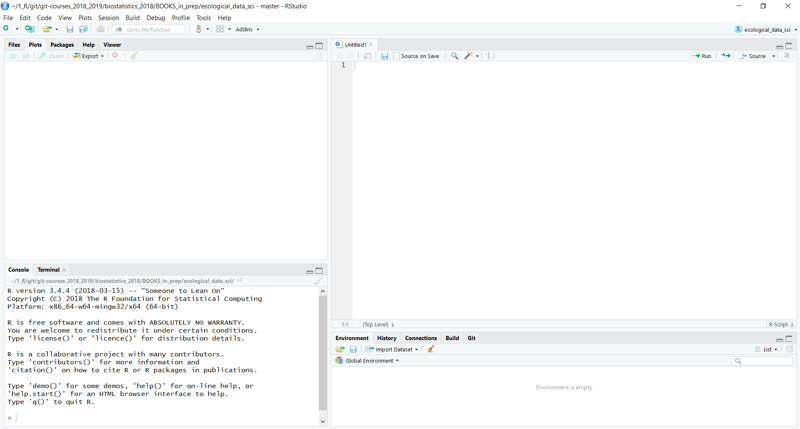
\includegraphics[width=11.11in]{C:/Users/lisanjie/Documents/1_R/git/git-teaching/teaching_2018_2019/2018_fall/biostats_fall_2018/4_biostats_bks_pkg/EDS/EDSbook/images/RStudio_1st_view-800x600} \caption{RStudio when first opened.}(\#fig:rstudio.open)
\end{figure}

When referring to RStudio, there are two terms that need to be
understood. As shown in Figure 3, there is the \textbf{console} section
of RStudio and the \textbf{script editor} or \textbf{source viewer}.

\begin{figure}
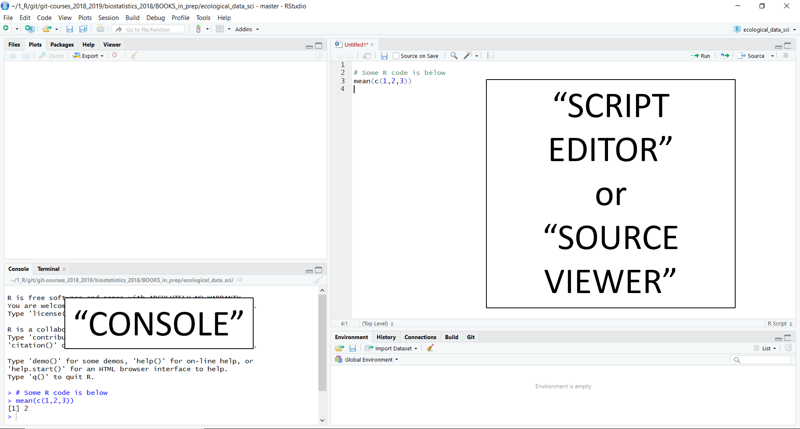
\includegraphics[width=11.11in]{C:/Users/lisanjie/Documents/1_R/git/git-teaching/teaching_2018_2019/2018_fall/biostats_fall_2018/4_biostats_bks_pkg/EDS/EDSbook/images/RStudio_console_vs_script_editor-800x600} \caption{RStudio's console and script editor.}(\#fig:rstudio.console)
\end{figure}

A ``cheat sheet'' called the ``RStudio IDE Cheat Sheet'' details all of
RStudio's many features and is available at
\url{https://www.rstudio.com/resources/cheatsheets/} . It very thorough,
though a bit dense.

\subsection{The console versus the script
editor}\label{the-console-versus-the-script-editor}

You can type and enter text into both the console and the script editor.
The console, however, respond like a calculator, while the script editor
works more like a text editor.

\subsubsection{The R console}\label{the-r-console}

The \textbf{console} in RStudio act exactly the same way as it does in
R. This is an \textbf{interactive programming} situation that is very
similar to a scientific calculator. If you click your mouse inside the
console and type ``1 + 1'' then press enter you will see the following
type of output

\begin{Shaded}
\begin{Highlighting}[]
\DecValTok{1} \OperatorTok{+}\StringTok{ }\DecValTok{1}
\end{Highlighting}
\end{Shaded}

\begin{verbatim}
## [1] 2
\end{verbatim}

Note that right in front of where you typed ``1+1'' there is a
``\textgreater{}'' symbol. This is always in the R console and never
needs to be typed.

One thing to note about R is that it's not particular about spacing. All
of the following things will yield the same results

\begin{Shaded}
\begin{Highlighting}[]
\DecValTok{1}\OperatorTok{+}\DecValTok{1}
\DecValTok{1} \OperatorTok{+}\StringTok{ }\DecValTok{1}
\DecValTok{1}          \OperatorTok{+}\StringTok{        }\DecValTok{1}
\end{Highlighting}
\end{Shaded}

\subsubsection{R's console as a scientific
calculator}\label{rs-console-as-a-scientific-calculator}

You can interact with R's console similar to a scientific calculator.
For example, you can use parentheses to set up mathematical statements
like

\begin{Shaded}
\begin{Highlighting}[]
\DecValTok{5}\OperatorTok{*}\NormalTok{(}\DecValTok{1}\OperatorTok{+}\DecValTok{1}\NormalTok{)}
\end{Highlighting}
\end{Shaded}

\begin{verbatim}
## [1] 10
\end{verbatim}

Note however that you have to be explicit about multiplication. If you
try the following it won't work.

\begin{Shaded}
\begin{Highlighting}[]
\DecValTok{5}\NormalTok{(}\DecValTok{1}\OperatorTok{+}\DecValTok{1}\NormalTok{)}
\end{Highlighting}
\end{Shaded}

R also has built-in functions that work similar to what you might have
used in Excel. For example, in Excel you can calculate the average of a
set of numbers by typing ``=average(1,2,3)'' into a cell. R can do the
same thing except

\begin{itemize}
\tightlist
\item
  The command is ``mean''
\item
  You don't start with ``=''
\item
  You have to package up the numbers like what is shown below using
  ``c(\ldots{})''
\end{itemize}

\begin{Shaded}
\begin{Highlighting}[]
\KeywordTok{mean}\NormalTok{(}\KeywordTok{c}\NormalTok{(}\DecValTok{1}\NormalTok{,}\DecValTok{2}\NormalTok{,}\DecValTok{3}\NormalTok{))}
\end{Highlighting}
\end{Shaded}

\begin{verbatim}
## [1] 2
\end{verbatim}

Where ``c(\ldots{})'' packages up the numbers the way the mean()
function wants to see them.

If you just do the following R will give you an answer, but its the
wrong one

\begin{Shaded}
\begin{Highlighting}[]
\KeywordTok{mean}\NormalTok{(}\DecValTok{1}\NormalTok{,}\DecValTok{2}\NormalTok{,}\DecValTok{3}\NormalTok{)}
\end{Highlighting}
\end{Shaded}

\textbf{This is a common issue with R -- and many programs, really -- it
won't always tell you when somethind didn't go as planned. This is
because it doesn't know something didn't go as planned; you have to
learn the rules R plays by.}

\subsubsection{Practice: math in the
console}\label{practice-math-in-the-console}

See if you can reproduce the following results

\textbf{Division}

\begin{Shaded}
\begin{Highlighting}[]
\DecValTok{10}\OperatorTok{/}\DecValTok{3}
\end{Highlighting}
\end{Shaded}

\begin{verbatim}
## [1] 3.333333
\end{verbatim}

\textbf{The standard deviation}

\begin{Shaded}
\begin{Highlighting}[]
\KeywordTok{sd}\NormalTok{(}\KeywordTok{c}\NormalTok{(}\DecValTok{5}\NormalTok{,}\DecValTok{10}\NormalTok{,}\DecValTok{15}\NormalTok{)) }\CommentTok{# note the use of "c(...)"}
\end{Highlighting}
\end{Shaded}

\begin{verbatim}
## [1] 5
\end{verbatim}

\subsubsection{The script editor}\label{the-script-editor}

While you can interact with R directly within the console, the standard
way to work in R is to write what are known as \textbf{scripts.} These
are computer code instructions written to R in a \textbf{script file.}
These are save with the extension \textbf{.R} but area really just a
form of \textbf{plain text file.}

To work with scripts, what you do is type commands in the script editor,
then tell R to \textbf{excute} the command. This can be done several
ways.

First, you tell RStudio the line of code you want to run by either *
Placing the cursor at the end a line of code, OR * Clicking and dragging
over the code you want to run in order highlight it.

Second, you tell RStudio to run the code by * Clicking the ``Run'' icon
in the upper right hand side of the script editor (a grey box with a
green error emerging from it) * pressing the control key (``ctrl)'' and
then then enter key on the keyboard

The code you've chosen to run will be sent by RStudio from the script
editor over to the console. The console will show you both the code and
then the output.

You can run several lines of code if you want; the console will run a
line, print the output, and then run the next line. First I'll use the
command mean(), and then the command sd() for the standard deviation:

\begin{Shaded}
\begin{Highlighting}[]
\KeywordTok{mean}\NormalTok{(}\KeywordTok{c}\NormalTok{(}\DecValTok{1}\NormalTok{,}\DecValTok{2}\NormalTok{,}\DecValTok{3}\NormalTok{))}
\end{Highlighting}
\end{Shaded}

\begin{verbatim}
## [1] 2
\end{verbatim}

\begin{Shaded}
\begin{Highlighting}[]
\KeywordTok{sd}\NormalTok{(}\KeywordTok{c}\NormalTok{(}\DecValTok{1}\NormalTok{,}\DecValTok{2}\NormalTok{,}\DecValTok{3}\NormalTok{))}
\end{Highlighting}
\end{Shaded}

\begin{verbatim}
## [1] 1
\end{verbatim}

\subsubsection{Comments}\label{comments}

One of the reasons we use script files is that we can combine R code
with \textbf{comments} that tell us what the R code is doing. Comments
are preceded by the hashtag symbol \textbf{\#}. Frequently we'll write
code like this:

\begin{Shaded}
\begin{Highlighting}[]
\CommentTok{#The mean of 3 numbers}
\KeywordTok{mean}\NormalTok{(}\KeywordTok{c}\NormalTok{(}\DecValTok{1}\NormalTok{,}\DecValTok{2}\NormalTok{,}\DecValTok{3}\NormalTok{))}
\end{Highlighting}
\end{Shaded}

If you highlight all of this code (including the comment) and then click
on ``run'', you'll see that RStudio sends all of the code over console.

\begin{verbatim}
## [1] 2
\end{verbatim}

Comments can also be placed at the \emph{end} of a line of code

\begin{Shaded}
\begin{Highlighting}[]
\KeywordTok{mean}\NormalTok{(}\KeywordTok{c}\NormalTok{(}\DecValTok{1}\NormalTok{,}\DecValTok{2}\NormalTok{,}\DecValTok{3}\NormalTok{)) }\CommentTok{#Note  the use of c(...)}
\end{Highlighting}
\end{Shaded}

Sometimes we write code and then don't want R to run it. We can prevent
R from executing the code even if its sent to the console by putting a
``\#'' \emph{infront} of the code.

If I run this code, I will get just the mean but not the sd.

\begin{Shaded}
\begin{Highlighting}[]
\KeywordTok{mean}\NormalTok{(}\KeywordTok{c}\NormalTok{(}\DecValTok{1}\NormalTok{,}\DecValTok{2}\NormalTok{,}\DecValTok{3}\NormalTok{))}
\CommentTok{#sd(c(1,2,3))}
\end{Highlighting}
\end{Shaded}

Doing this is called \textbf{commenting out} a line of code.

\section{Help!}\label{help}

There are many resource for figuring out R and RStudio, including

\begin{itemize}
\tightlist
\item
  R's built in ``help'' function
\item
  Q\&A websites like \textbf{stackoverflow.com}
\item
  twitter, using the hashtag \#rstats
\item
  blogs
\item
  online books and course materials
\end{itemize}

\subsection{\texorpdfstring{Getting ``help'' from
R}{Getting help from R}}\label{getting-help-from-r}

If you are using a function in R you can get info about how it works
like this

\begin{Shaded}
\begin{Highlighting}[]
\NormalTok{?mean}
\end{Highlighting}
\end{Shaded}

In RStudio the help screen should appear, probably above your console.
If you start reading this help file, though, you don't have to go far
until you start seeing lots of R lingo, like ``S3 method'',``na.rm'',
``vectors''. Unfortunately, the R help files are usually not written for
beginners, and reading help files is a skill you have to acquire.

For example, when we load data into R in subsequent lessons we will use
a function called ``read.csv''

Access the help file by typing ``?read.csv'' into the console and
pressing enter. Surprisingly, the function that R give you the help file
isn't what you asked for, but is read.table(). This is a related
function to read.csv, but when you're a beginner thing like this can
really throw you off.

Kieran Healy as produced a great cheatsheet for reading R's help pages
as part of his forthcoming book. It should be available online at
\url{http://socviz.co/appendix.html\#a-little-more-about-r}

\subsection{Getting help from the
internet}\label{getting-help-from-the-internet}

The best way to get help for any topic is to just do an internet search
like this: ``R read.csv''. Usually the first thing on the results list
will be the R help file, but the second or third will be a blog post or
something else where a usually helpful person has discussed how that
function works.

Sometimes for very basic R commands like this might not always be
productive but its always work a try. For but things related to stats,
plotting, and programming there is frequently lots of information. Also
try searching YouTube.

\subsection{Getting help from online
forums}\label{getting-help-from-online-forums}

Often when you do an internet search for an R topic you'll see results
from the website www.stackoverflow.com, or maybe www.crossvalidated.com
if its a statistics topic. These are excellent resources and many
questions that you may have already have answers on them. Stackoverflow
has an internal search function and also suggests potentially relevant
posts.

Before posting to one of these sites yourself, however, do some
research; there is a particular type and format of question that is most
likely to get a useful response. Sadly, people new to the site often get
``flamed'' by impatient pros.

\subsection{Getting help from twitter}\label{getting-help-from-twitter}

Twitter is a surprisingly good place to get information or to find other
people knew to R. Its often most useful to ask people for learning
resources or general reference, but you can also post direct questions
and see if anyone responds, though usually its more advanced users who
engage in twitter-based code discussion.

A standard tweet might be ``Hey \#rstats twitter, am knew to \#rstats
and really stuck on some of the basics. Any suggestions for good
resources for someone starting from scratch?''

\section{Other features of RStudio}\label{other-features-of-rstudio}

\subsection{Ajusting pane the layout}\label{ajusting-pane-the-layout}

You can adjust the location of each of RStudio 4 window panes, as well
as their size.

To set the pane layout go to 1. ''Tools'' on the top menu 1. ''Global
options'' 1. ``Pane Layout''

Use the drop-down menus to set things up. I recommend 1. Lower left:
``Console''" 1. Top right: ``Source'' 1. Top left: ``Plot, Packages,
Help Viewer'' 1. This will leave the ``Environment\ldots{}'' panel in
the lower right.

\subsection{Adjusting size of windows}\label{adjusting-size-of-windows}

You can clicked on the edge of a pane and adjust its size. For most R
work we want the console to be big. For beginners, the ``Environment,
history, files'' panel can be made really small.

\section{Practice (OPTIONAL)}\label{practice-optional}

Practice the following operations. Type the directly into the console
and execute them. Also write them in a script in the script editor and
run them.

\textbf{Square roots}

\begin{Shaded}
\begin{Highlighting}[]
\KeywordTok{sqrt}\NormalTok{(}\DecValTok{42}\NormalTok{)}
\end{Highlighting}
\end{Shaded}

\begin{verbatim}
## [1] 6.480741
\end{verbatim}

\textbf{The date} Some functions in R can be executed within nothing in
the parentheses.

\begin{Shaded}
\begin{Highlighting}[]
\KeywordTok{date}\NormalTok{()}
\end{Highlighting}
\end{Shaded}

\begin{verbatim}
## [1] "Thu Sep 06 15:56:10 2018"
\end{verbatim}

\textbf{Exponents} The \textbf{\^{}} is used for exponents

\begin{Shaded}
\begin{Highlighting}[]
\DecValTok{42}\OperatorTok{^}\DecValTok{2}
\end{Highlighting}
\end{Shaded}

\begin{verbatim}
## [1] 1764
\end{verbatim}

\textbf{A series of numbers} A colon between two numbers creates a
series of numbers.

\begin{Shaded}
\begin{Highlighting}[]
\DecValTok{1}\OperatorTok{:}\DecValTok{42}
\end{Highlighting}
\end{Shaded}

\begin{verbatim}
##  [1]  1  2  3  4  5  6  7  8  9 10 11 12 13 14 15 16 17 18 19 20 21 22 23
## [24] 24 25 26 27 28 29 30 31 32 33 34 35 36 37 38 39 40 41 42
\end{verbatim}

\textbf{logs} The default for the log() function is the natural log.

\begin{Shaded}
\begin{Highlighting}[]
\KeywordTok{log}\NormalTok{(}\DecValTok{42}\NormalTok{)}
\end{Highlighting}
\end{Shaded}

\begin{verbatim}
## [1] 3.73767
\end{verbatim}

log10() gives the base-10 log.

\begin{Shaded}
\begin{Highlighting}[]
\KeywordTok{log10}\NormalTok{(}\DecValTok{42}\NormalTok{)}
\end{Highlighting}
\end{Shaded}

\begin{verbatim}
## [1] 1.623249
\end{verbatim}

\textbf{exp() raises e to a power}

\begin{Shaded}
\begin{Highlighting}[]
\KeywordTok{exp}\NormalTok{(}\FloatTok{3.73767}\NormalTok{)}
\end{Highlighting}
\end{Shaded}

\begin{verbatim}
## [1] 42.00002
\end{verbatim}

\textbf{Multiple commands can be nested}

\begin{Shaded}
\begin{Highlighting}[]
\KeywordTok{sqrt}\NormalTok{(}\DecValTok{42}\NormalTok{)}\OperatorTok{^}\DecValTok{2}
\KeywordTok{log}\NormalTok{(}\KeywordTok{sqrt}\NormalTok{(}\DecValTok{42}\NormalTok{)}\OperatorTok{^}\DecValTok{2}\NormalTok{)}
\KeywordTok{exp}\NormalTok{(}\KeywordTok{log}\NormalTok{(}\KeywordTok{sqrt}\NormalTok{(}\DecValTok{42}\NormalTok{)}\OperatorTok{^}\DecValTok{2}\NormalTok{))}
\end{Highlighting}
\end{Shaded}

\chapter{The different faces of R code: The console, scripts \&
RMarkdown}\label{the-different-faces-of-r-code-the-console-scripts-rmarkdown}

There are a number of ways to interact with R

\begin{itemize}
\tightlist
\item
  Directly in the \textbf{console}, like a scientific calculator
\item
  Using \textbf{script files} (.R) with
\item
  R code types out and sent over to the console
\item
  notes ``commented out'' using hastags ``\#''
\item
  \textbf{rmarkdown} (.Rmd) files with
\item
  R code in species \textbf{code chunks}
\item
  notes written like in a word precessor
\item
  formatting using \textbf{markdown}, a \textbf{markup language}
\end{itemize}

This chapter will briefly introduce these different ways of working in R

\section{The console}\label{the-console}

In a previous chapter we introduced the \textbf{console.} You can
interact with the console in a similar manner as a scientific
calculator.

\begin{figure}
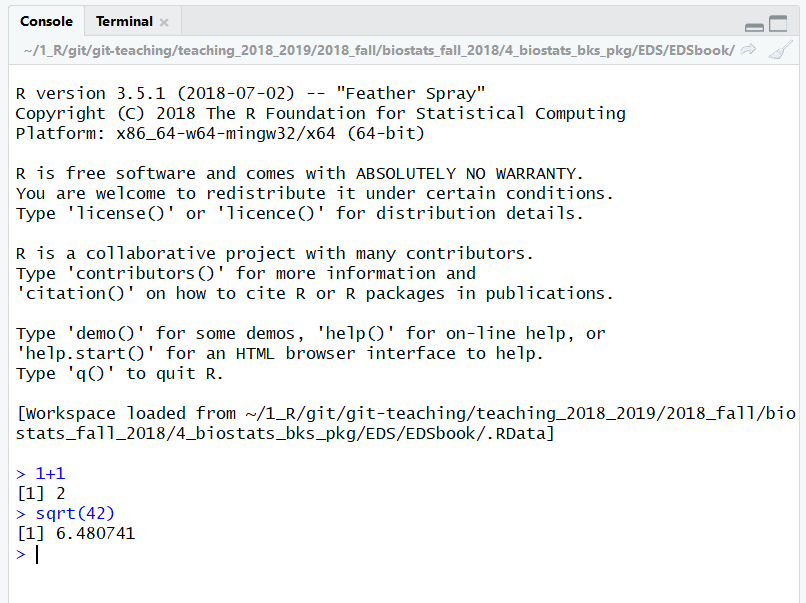
\includegraphics[width=11.19in]{C:/Users/lisanjie/Documents/1_R/git/git-teaching/teaching_2018_2019/2018_fall/biostats_fall_2018/4_biostats_bks_pkg/EDS/EDSbook/images/RStudio_console} \caption{The RStudio console}(\#fig:first.chnk.sxn1ch4)
\end{figure}

As you execute more commands, the move up the screen. You can scroll
back up to see what you've done previously.

\section{Scripts}\label{scripts}

You can create a record of the commands you have executed in the
console, but this isn't a very efficient way to work. If you want to
keep track of the commands you're running (and often you do) its best to
write them in a script file and then send them over to the console to
execute the code.

\subsection{Creating scripts}\label{creating-scripts}

When you open RStudio a blank script file will be open. Subsequently,
RStudio will open files you have worked with previously. To create a new
blank script file:

\begin{itemize}
\tightlist
\item
  Click on File
\item
  New File
\item
  R script
\end{itemize}

or just type control + shift + N (on a PC) or command + shift + N on
(?on mac), which is similar how you make a new document in most
programs.

\begin{figure}
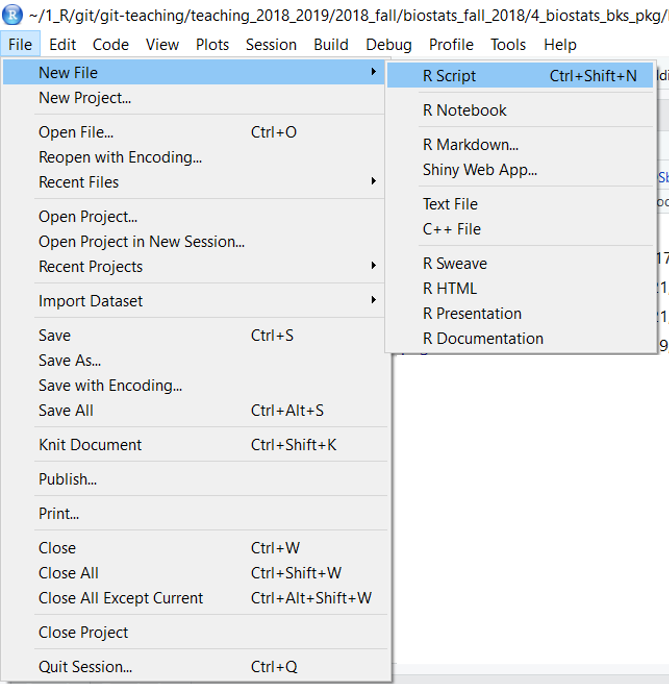
\includegraphics[width=9.31in]{C:/Users/lisanjie/Documents/1_R/git/git-teaching/teaching_2018_2019/2018_fall/biostats_fall_2018/4_biostats_bks_pkg/EDS/EDSbook/images/Rstudio_new_R_script} \caption{Creating a new R script file}\label{fig:unnamed-chunk-23}
\end{figure}

You can create or open multiple scripts, which RStudio organizes as tabs
like in a web browser.

\begin{figure}
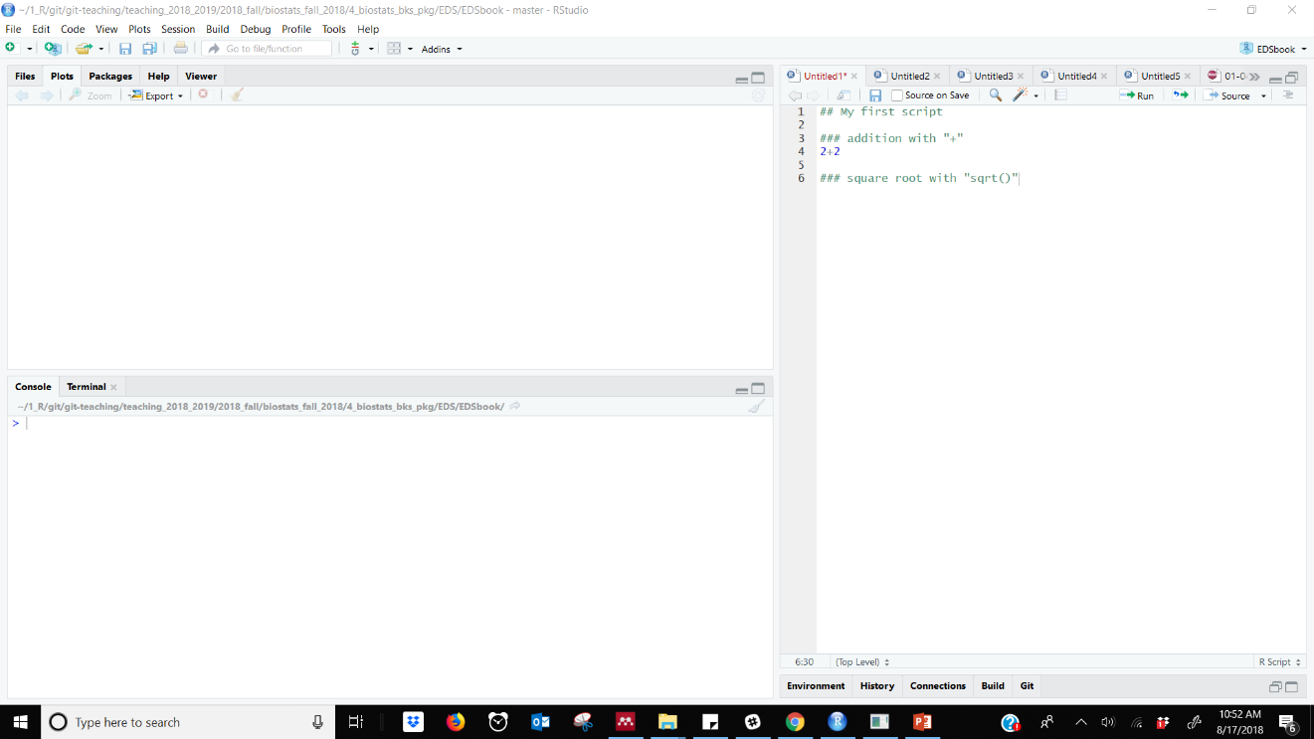
\includegraphics[width=18.25in]{C:/Users/lisanjie/Documents/1_R/git/git-teaching/teaching_2018_2019/2018_fall/biostats_fall_2018/4_biostats_bks_pkg/EDS/EDSbook/images/Rstudio_scripts} \caption{R Script file with comments in RStudio}\label{fig:unnamed-chunk-24}
\end{figure}

\subsection{Running code from a
script}\label{running-code-from-a-script}

To run a code you can either place click to the righ of the line of code
and click the ``run'' button.

\begin{figure}
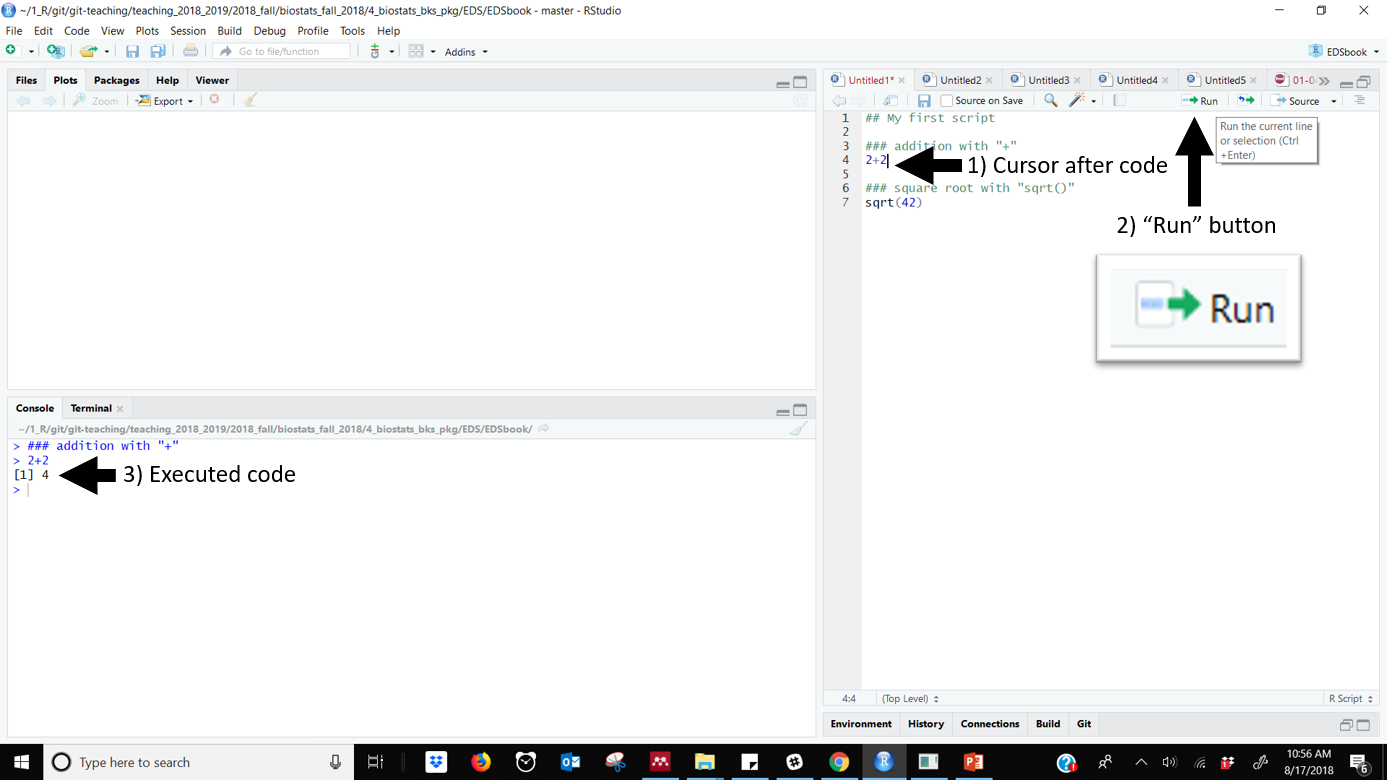
\includegraphics[width=19.26in]{C:/Users/lisanjie/Documents/1_R/git/git-teaching/teaching_2018_2019/2018_fall/biostats_fall_2018/4_biostats_bks_pkg/EDS/EDSbook/images/RStudios_RUN_button} \caption{Running code using RStudios RUN button.  Note cursor to the right of the code}\label{fig:unnamed-chunk-25}
\end{figure}

You can also highlight the code by clicking and dragging over it. This
is useful when you have multiple lines of code.

\begin{figure}
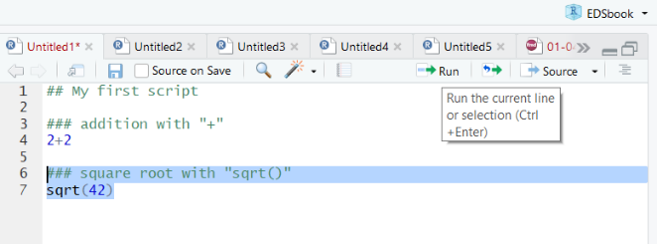
\includegraphics[width=9.12in]{C:/Users/lisanjie/Documents/1_R/git/git-teaching/teaching_2018_2019/2018_fall/biostats_fall_2018/4_biostats_bks_pkg/EDS/EDSbook/images/RStudio_script_code_highlighted} \caption{Highlighted code in an RStudio script}\label{fig:unnamed-chunk-26}
\end{figure}

\subsection{Running code with keyboard
shortcuts}\label{running-code-with-keyboard-shortcuts}

Want to look like an R pro? Learn keyboard shortcuts so you don't have
to use the mouse. Both of the above methods work using simple keyboard
shortcuts:

\begin{itemize}
\tightlist
\item
  PCs: Control + Enter
\item
  Macs: Command + Enter (?)
\end{itemize}

Another handy shortcut is ``Control + 2'', which moves your computer's
cursor from the script editor to the console. (Control + 2 moves it from
console to editor)

\section{Organizing scripts}\label{organizing-scripts}

\begin{quote}
``You mostly collaborate with yourself, and me-from-two-months-ago never
responds to email.''
(\href{https://twitter.com/kcranstn/statuses/370914072511791104}{Karen
Cranston}, paraphrasing Mark Holder; quoted by Megan Duffy on
\href{https://dynamicecology.wordpress.com/2015/02/18/the-biggest-benefit-of-my-shift-to-r-reproducibility/}{dynamicecology})
\end{quote}

Script files perform a record of your work so you can

\begin{itemize}
\tightlist
\item
  remember what you did
\item
  re-run it to check things
\item
  re-use your code for new analyses
\item
  track down errors (which will happen!)
\item
  share with collaborators
\end{itemize}

Script files are not unique to R, but the R community seems to have
built up a particularly good infrasture for their implemenation and
ethos encouraging their use. Megan Duffey at
\href{https://dynamicecology.wordpress.com/2015/02/18/the-biggest-benefit-of-my-shift-to-r-reproducibility/}{Dynamic
Ecology} has an excellent post on this.

When you first start out learning R most of your scripts will be
disposable. Quickly you'll want to start keeping track of the code you
write in class to refer back to. When you start doing analyses you'll
want to write comments as you go, and provide details at the top of your
file so you can quickly get up to speed when you come back to the file.

\subsection{What to include in a
script}\label{what-to-include-in-a-script}

A good R script should be a self-sufficient document that your future
self can easily make sense of, or better yet, someone starting from
scratch can understand. Depending on the exact purpose, things to
include might be

\begin{itemize}
\tightlist
\item
  A general title, such as ``R Script: data exploration \&t-test for
  analaysis of frog arm girth''
\item
  Who wrote it and their contact info
\item
  When the script was created
\item
  when it was most recently accessed or created
\item
  What data it uses and where it comes from
\item
  What project or paper it relates to
\end{itemize}

A challenge when writing and maintaining R scripts is that you are often
actively engaged in learnign R, learning stats, and learning about or
exploring your data. So you write a lot of code then erase it, or
scratch out code in a script and then move on. While I have written and
saved many scripts that I have never re-opened, I have never re-opened a
script and said ``wow, I went WAY overboard annotating this thing!''
ALso, commenting code makes it much easier to read; I often add fairly
simple comments to make code easier navigate and to break things up into
smaller chunks.

So, at a minimum I think every script should

\begin{itemize}
\tightlist
\item
  Have some kind of header saying what it is and when it was made
\item
  Have one line of comments or annotations for every 3 to 5 lines of
  code.
\end{itemize}

\subsection{Formatting sections in R
scripts}\label{formatting-sections-in-r-scripts}

To make scripts easier to navigate its useful to strong together the
comment character ``\#'' to make dividers and boxes. This is very good
practice to make code more readable. It can be a bit tedious at times to
do this; one advantage of rmarkdown, which we'll introduce at the end of
this chapter and go into further in the next, is that it makes it very
easy to format section titles.

\subsection{A sample R script}\label{a-sample-r-script}

On the following pages are examples of R scripts for a formal analysis
of a dataset. First I'll show what the script might look like as I write
it. Then I'll show how I'll fix it up once I know its something I am
going to look back at in the fugure

\begin{Shaded}
\begin{Highlighting}[]
\NormalTok{### R Script: Analysis of frog arm girth}

\NormalTok{## Nathan Brouwer (brouwern@gmail.com)}
\NormalTok{## 6/6/2018}
\NormalTok{## update: 8/17/2018}

\NormalTok{## I am re-running analysis from paper by Buzatto  et al 2015}
\NormalTok{## I want to compare the results of a t-test with}
\NormalTok{## and w/o Welche's correction for unequal variation}

\NormalTok{## Packages}
\KeywordTok{library}\NormalTok{(wildlifeR)}

\NormalTok{## Data set up}
\CommentTok{# load frogarm data from Buzatto et al 2015}
\KeywordTok{data}\NormalTok{(}\StringTok{"frogarms"}\NormalTok{)}


\NormalTok{## Data visualization}
\CommentTok{# histogram of all data}
\KeywordTok{hist}\NormalTok{(frogarms}\OperatorTok{$}\NormalTok{sv.length)}
\end{Highlighting}
\end{Shaded}

\begin{Shaded}
\begin{Highlighting}[]
\NormalTok{## Data analysis}
\CommentTok{# unpaired t-test NOT using Welch's correction}
\NormalTok{## }\AlertTok{NOTE}\NormalTok{: assumes variation within each group EQUAL}
\KeywordTok{t.test}\NormalTok{(sv.length }\OperatorTok{~}\StringTok{ }\NormalTok{sex,   }\CommentTok{# model formula}
       \DataTypeTok{var.equal =} \OtherTok{TRUE}\NormalTok{,  }\CommentTok{# set variances to equal }
         \DataTypeTok{data =}\NormalTok{ frogarms) }\CommentTok{# data}

\CommentTok{# unpaired t-test >>using<< Welch's correctin}
\KeywordTok{t.test}\NormalTok{(sv.length }\OperatorTok{~}\StringTok{ }\NormalTok{sex, }
       \DataTypeTok{var.equal =} \OtherTok{FALSE}\NormalTok{, }\CommentTok{# set variances to be unequal }
         \DataTypeTok{data =}\NormalTok{ frogarms)}
\end{Highlighting}
\end{Shaded}

\subsection{A polished R script}\label{a-polished-r-script}

\begin{Shaded}
\begin{Highlighting}[]
\NormalTok{###########################################}
\NormalTok{###}
\NormalTok{### R Script: Analysis of frog arm girth}
\NormalTok{###}
\NormalTok{###########################################}

\NormalTok{## Author:      Nathan Brouwer (brouwern@gmail.com)}
\NormalTok{## Creation:    6/6/2018}
\NormalTok{## Last update: 8/17/2018}


\NormalTok{###############}
\NormalTok{## Introduction}
\NormalTok{###############}

\CommentTok{# This script is an analysis of frog body size and arm girth}

\NormalTok{## I am re-running analysis from paper by Buzatto  et al 2015}
\NormalTok{## I want to compare the results of a t-test with}
\NormalTok{## and w/o Welche's correction for unequal variation}
\end{Highlighting}
\end{Shaded}

\begin{Shaded}
\begin{Highlighting}[]
\CommentTok{# Data were originally from }
\CommentTok{# Buzatto  et al 2015. Sperm competition and the evolution of }
\CommentTok{#       precopulatory weapons: Increasing male density promotes}
\CommentTok{#       sperm competition and reduces selection on arm strength in}
\CommentTok{#       a chorusing frog. Evolution 69: 2613-2624. }
\CommentTok{#       https://doi.org/10.1111/evo.12766}

\CommentTok{# Data originally downloaded on  6/6/2018 from}
\CommentTok{#   https://figshare.com/articles/Data_Paper_Data_Paper/3554424}

\CommentTok{# Data are included in the wildlifeR package and load from it}
\CommentTok{#     https://github.com/brouwern/wildlifeR}
\end{Highlighting}
\end{Shaded}

\begin{Shaded}
\begin{Highlighting}[]
\NormalTok{###############}
\NormalTok{## Packages}
\NormalTok{###############}

\KeywordTok{library}\NormalTok{(wildlifeR)}

\NormalTok{###############}
\NormalTok{## Data set up}
\NormalTok{###############}

\CommentTok{# load frogarm data from Buzatto et al 2015}
\KeywordTok{data}\NormalTok{(}\StringTok{"frogarms"}\NormalTok{)}

\NormalTok{######################}
\NormalTok{## Data visualization}
\NormalTok{######################}

\CommentTok{# histogram of all data}
\KeywordTok{hist}\NormalTok{(frogarms}\OperatorTok{$}\NormalTok{sv.length)}
\end{Highlighting}
\end{Shaded}

\begin{Shaded}
\begin{Highlighting}[]
\NormalTok{######################}
\NormalTok{## Data analysis}
\NormalTok{######################}

\CommentTok{# unpaired t-test NOT using Welch's correction}
\NormalTok{## }\AlertTok{NOTE}\NormalTok{: assumes variation within each group EQUAL}
\KeywordTok{t.test}\NormalTok{(sv.length }\OperatorTok{~}\StringTok{ }\NormalTok{sex,   }\CommentTok{# model formula}
       \DataTypeTok{var.equal =} \OtherTok{TRUE}\NormalTok{,  }\CommentTok{# set variances to equal }
         \DataTypeTok{data =}\NormalTok{ frogarms) }\CommentTok{# data}

\CommentTok{# unpaired t-test >>using<< Welch's correctin}
\KeywordTok{t.test}\NormalTok{(sv.length }\OperatorTok{~}\StringTok{ }\NormalTok{sex, }
       \DataTypeTok{var.equal =} \OtherTok{FALSE}\NormalTok{, }\CommentTok{# set variances to be unequal }
         \DataTypeTok{data =}\NormalTok{ frogarms)}
\end{Highlighting}
\end{Shaded}

For more on organizing scripts see points 4 and 5 of ``Eight things I do
to make my open research more findable and understandable'' at
(DataColada{]}(\url{http://datacolada.org/69}).

\section{RMarkdown}\label{rmarkdown}

{[}this section has not been completed{]}

\begin{itemize}
\tightlist
\item
  File
\item
  New File
\item
  R Markdown
\end{itemize}

A pop up menu will appear with lots of options; just click ``ok.''

\chapter{RMarkdown}\label{rmarkdown-1}

{[}this chapter has not been written : ( {]}

\section{\texorpdfstring{The ``YAML''
Header}{The YAML Header}}\label{the-yaml-header}

\section{Word processing}\label{word-processing}

\section{\texorpdfstring{Code
``chunks''}{Code chunks}}\label{code-chunks}

\part{Getting Software \& Data Into
R}\label{part-getting-software-data-into-r}

\subsection*{}\label{section-1}
\addcontentsline{toc}{subsection}{}

In this we'll discuss two of the most fundamental steps of data
analysis: getting your hard-earned data into the @\$*\%\# program you
want to do you analysis in. This is often one of the most frustrating
steps for beginners because R, like most data analysis tools that aren't
spreadsheets, it seemingly very picky about how it wants to receive
data. Luckily there's a method behind the madness, and also some handy
tools in RStudio to help with this.

Most data starts off as a spreadsheet before it enters R. Loading
spreadsheet data into R will be our end goal, but as a run up will step
through several easier tasks that will highlight the core principles of
getting data into R, in particular loading additional software into R
(called packages) and loading the data in those packages into R. We'll
also load data directly from the internet into R.

The chapters in this section are cover the following:

\begin{enumerate}
\def\labelenumi{\arabic{enumi}.}
\tightlist
\item
  Loading R packages to get new software into R
\item
  Loading and looking at data from R packages
\item
  Loading packages from the software repository GitHub
\item
  Loading data from the internet
\item
  Loading spreadsheets as .csv files
\item
  Loading Excel spreadsheets
\end{enumerate}

\chapter{Loading packages from CRAN}\label{loading-packages-from-cran}

\textbf{Nathan Brouwer, Phd}\\
brouwern at gmail.com\\
\url{https://github.com/brouwern}\\
Twitter: lobrowR

\section{Introduction}\label{introduction}

When you install R you get \textbf{base R}, which is the core set of
functions, functionality, and some data sets. Base R however is
surrounded by a universe of extensions built by statistician,
programmers, academics and businesses that use R for analyses. A lot of
R's functionality is found in these packages, including data sets,
special plotting functions, and statistical tools for the analysis of
complex data. Some of these are fairly standard and are downloaded along
with base R and just need to be explicitly installed. Other have to be
downloaded from the internet and installed. Most packages contain data
in order to demonstrate what they do; working with data from packages
will be covered in a later lesson.

This book relies heavily on an R package I've written called
``wildlifeR'' (\url{https://brouwern.github.io/wildlifeR/}) that
contains the datasets used throughout the book, as well as some helpful
R functions I've written.

Most R packages you'll use are stored on the CRAN website where you
download R (\url{https://cran.r-project.org/}). R and RStudio have
functions and tools for downloading and managing packages that we'll
briefly introduce in this exercise.

Another place a package can be stored online is a code repository like
GitHub. The wildlifeR package lives on GitHub and can be downloaded
directly from there. Many packages on CRAN also occur on GitHub,
especially if programmers are actively developing, updating, and
managing the package. We'll cover downloading packages from GitHub in
the next exercise.

\subsection{Learning objectives}\label{learning-objectives}

This exercise will introduce students to

\begin{enumerate}
\def\labelenumi{\arabic{enumi}.}
\tightlist
\item
  the concept of an \textbf{R Package} (aka \textbf{library})
\item
  how to load R packages using the library() function
\item
  the R plotting package \textbf{ggplot2}
\item
  cool add-ons to ggplot2, \textbf{ggpubr} and \textbf{cowplot}
\end{enumerate}

\subsection{Learning goals}\label{learning-goals}

By the end of this exercise students should be able to

\begin{itemize}
\tightlist
\item
  locate and download packages from the CRAN website using RStudio
\item
  recognize the R functions used to download and install packages.
\end{itemize}

\subsection{Functions \& Arguements}\label{functions-arguements}

\begin{itemize}
\tightlist
\item
  install.packages
\item
  dependencies = TRUE
\item
  library
\end{itemize}

\subsection{Packages}\label{packages}

\begin{itemize}
\tightlist
\item
  MASS
\item
  ggplot2
\item
  ggpubr
\item
  cowplot
\end{itemize}

\subsection{Potential hangups}\label{potential-hangups}

\begin{itemize}
\tightlist
\item
  quoted vs.~unquoted text (eg qplot vs.~ggpubr syntax)
\end{itemize}

\section{Loading packages that come with base
R}\label{loading-packages-that-come-with-base-r}

What you download from CRAN is \textbf{base R} (also known as the
\textbf{base distribution}). Many functions are called \textbf{base
functions} because they are hard-wired into R.

\begin{center}\rule{0.5\linewidth}{\linethickness}\end{center}

\section{OPTIONAL: What functions come with base
R?}\label{optional-what-functions-come-with-base-r}

\textbf{The following section is opitonal}

If for some reason you want to see \emph{all} the functions that come
with base R, type this into the console and press enter. (ls stands for
``list'' and is a function we'll use more later).

\begin{Shaded}
\begin{Highlighting}[]
\KeywordTok{ls}\NormalTok{(}\StringTok{"package:base"}\NormalTok{)}
\end{Highlighting}
\end{Shaded}

As R has been developed there has also built up a cannon of tried and
true packages that are downloaded automatically when you download R, but
they aren't brought into R's working memory unless you tell R.

\section{Optional: What packages come with base
R?}\label{optional-what-packages-come-with-base-r}

\begin{quote}
If you want to see all of the packages that come with base R, do this.
library() is a function you will use a lot.
\end{quote}

\begin{Shaded}
\begin{Highlighting}[]
\KeywordTok{.libPaths}\NormalTok{(}\StringTok{""}\NormalTok{) }
\KeywordTok{library}\NormalTok{()}
\end{Highlighting}
\end{Shaded}

One package that is part of this cannon is MASS, which stands for Modern
Applied Statistics in S. ``S'' is the precursor to R, and MASS is the
package that accompanies the book of the same name, which is one of the
original books on S/R.
(\url{https://www.springer.com/us/book/9780387954578})

\textbf{End optional section}

\begin{center}\rule{0.5\linewidth}{\linethickness}\end{center}

\subsection{\texorpdfstring{\protect\hyperlink{section-3}{} Loading
packages with the library()
function}{ Loading packages with the library() function}}\label{loading-packages-with-the-library-function}

When a function is already downloaded to your computer, you explicitly
load it into R's working memory using the library() command.

\begin{Shaded}
\begin{Highlighting}[]
\KeywordTok{library}\NormalTok{(MASS)}
\end{Highlighting}
\end{Shaded}

\subsection{Preview: loading data from
packages}\label{preview-loading-data-from-packages}

Many packages have data. We can load data using the data() command.

\begin{Shaded}
\begin{Highlighting}[]
\KeywordTok{data}\NormalTok{(crabs)}
\end{Highlighting}
\end{Shaded}

We plot data with the plot() command.

\begin{Shaded}
\begin{Highlighting}[]
\KeywordTok{plot}\NormalTok{(FL }\OperatorTok{~}\StringTok{ }\NormalTok{RW, }\DataTypeTok{data =}\NormalTok{ crabs)}
\end{Highlighting}
\end{Shaded}

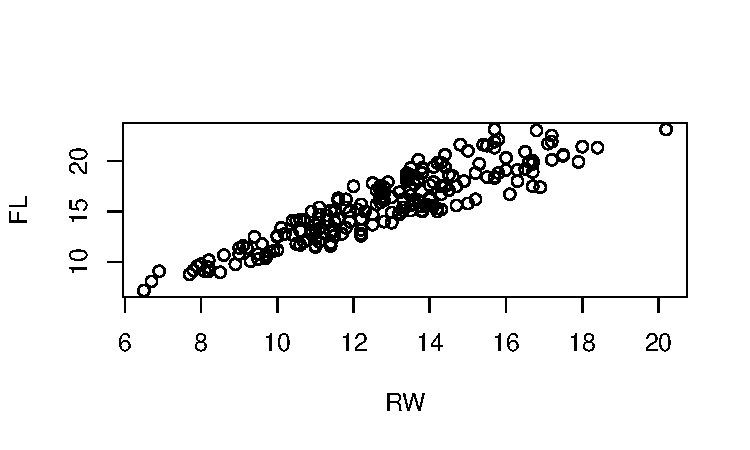
\includegraphics{bookdown-demo_files/figure-latex/unnamed-chunk-33-1.pdf}

\section{Load data from an external R
package}\label{load-data-from-an-external-r-package}

Many packages have to be explicitly downloaded and installed in order to
use their functions and datasets. Note that this is a \textbf{two-step
process}: 1. Download package from internet 1. Explicitly tell R to load
it

\subsection{\texorpdfstring{\protect\hyperlink{section-3}{} Step 1:
Downloading packages with
install.packages()}{ Step 1: Downloading packages with install.packages()}}\label{step-1-downloading-packages-with-install.packages}

There are a number of ways to download packages. One of the easiest is
to use the function install.packages(). Note that it might be better to
call this ``download.packages'' since after you install it, you also
have to load it!

Frequently in this book I will include install.packages(\ldots{}) at the
beginning of a lesson the first time we use a package to make sure the
package is downloaded. Note, however, that if you already have
downloaded the package, running install.packages(\ldots{}) will download
a new copy.

We'll download a package used for plotting called ggplot2, which stands
for ``Grammar of Graphics.''

\begin{Shaded}
\begin{Highlighting}[]
\KeywordTok{install.packages}\NormalTok{(}\StringTok{"ggplot2"}\NormalTok{)}
\end{Highlighting}
\end{Shaded}

Often when you download a package you'll see a fair bit of red text, and
sometime other things will pop up. Usually there's nothing of interest
here, but sometimes you need to read things carefully over it for hints
about why something didn't work.

\begin{center}\rule{0.5\linewidth}{\linethickness}\end{center}

\section{Optional: Seeing all of your installed
packages}\label{optional-seeing-all-of-your-installed-packages}

\textbf{The following section is optional}

If for some reason you want to see everything you've downloaded, do
this.

\begin{Shaded}
\begin{Highlighting}[]
\KeywordTok{installed.packages}\NormalTok{()}
\end{Highlighting}
\end{Shaded}

\textbf{End optional section}

\begin{center}\rule{0.5\linewidth}{\linethickness}\end{center}

\subsection{\texorpdfstring{\protect\hyperlink{section-3}{} Step 2:
Explicitly loading a package with
library()}{ Step 2: Explicitly loading a package with library()}}\label{step-2-explicitly-loading-a-package-with-library}

The install.packages() functions just saves the package software to R;
now you need to tell R ``I want to work with the package''. This is done
using the library() function. (Its called library because another name
for packages is libraries)

\begin{Shaded}
\begin{Highlighting}[]
\KeywordTok{library}\NormalTok{(ggplot2)}
\end{Highlighting}
\end{Shaded}

\begin{center}\rule{0.5\linewidth}{\linethickness}\end{center}

\section{OPTIONAL: Making a plot with
ggplot}\label{optional-making-a-plot-with-ggplot}

\textbf{This section is optional}

Now we can make a plot with the ggplot2 package we just downloaded, like
using the qplot() function. (Note that the syntax is different than what
we did above with plot() ).*

\begin{Shaded}
\begin{Highlighting}[]
\KeywordTok{qplot}\NormalTok{(}\DataTypeTok{y=}\NormalTok{FL, }\DataTypeTok{x=}\NormalTok{ RW, }\DataTypeTok{data =}\NormalTok{ crabs)}
\end{Highlighting}
\end{Shaded}

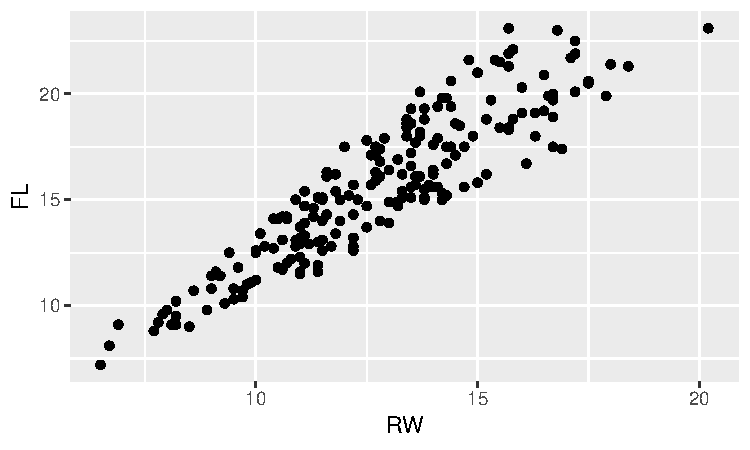
\includegraphics{bookdown-demo_files/figure-latex/unnamed-chunk-37-1.pdf}

\textbf{End opitional section}

\begin{center}\rule{0.5\linewidth}{\linethickness}\end{center}

\section{\texorpdfstring{\protect\hyperlink{section-3}{} Downloading
packages using
RStudio}{ Downloading packages using RStudio}}\label{downloading-packages-using-rstudio}

RStudio has a point-and-click interface to download packages. In the
pane that says ``Files, Plots, Packages, Help, Viewer'' click on
``Packages''. When the panel shift below ``Packages'' it will say
``Install, Update, Packrat.'' Click on ``Install.'' (There might be a
lag during this process as RStudio get info about your packages). In the
pop up widow there will be a middle field ``Packages'' where you can
type the name of your package. There's an auto-complete feature to help
you in case you forget the name. Then click ``install.'' Note that in
the bottom right corner of the pop up is a checked box next to ``Install
dependencies.'' Leave that checked; more on that later.

\section{\texorpdfstring{\protect\hyperlink{section-3}{} Packages \&
their
dependencies}{ Packages \& their dependencies}}\label{packages-their-dependencies}

R packages frequently use other R packages (which frequently use other R
packages\ldots{}). When an R package requires another package, its
called a \textbf{dependency.} Depending on who and how the package was
written up, dependencies might not be an issue or could be a problem.

As noted above when you download packages using RStudio's point and
click interface there's a box that should be checked called ``Install
dependencies.''

If you are using install.packages() there is an extra argument
``dependencies = TRUE'' that elicits the same behavior. I'll use this to
get an add-on for ggplot2 called ggpubr.

\begin{Shaded}
\begin{Highlighting}[]
\KeywordTok{install.packages}\NormalTok{(}\StringTok{"ggpubr"}\NormalTok{,}\DataTypeTok{dependencies =} \OtherTok{TRUE}\NormalTok{)}
\end{Highlighting}
\end{Shaded}

We can then install this

\begin{Shaded}
\begin{Highlighting}[]
\KeywordTok{library}\NormalTok{(ggpubr)}
\end{Highlighting}
\end{Shaded}

\begin{center}\rule{0.5\linewidth}{\linethickness}\end{center}

\section{Optional: Make a plot with
ggpubr}\label{optional-make-a-plot-with-ggpubr}

\textbf{This section is optional}

ggpubr is an add on to ggplot. (This means that ggpubr has ggplot as a
dependency). Note that the syntax for ggpubr function we use,
ggscatter(), has a different syntax (again) than ggplot's qplot()
function and base R's plot() function.

\begin{Shaded}
\begin{Highlighting}[]
\KeywordTok{ggscatter}\NormalTok{(}\DataTypeTok{data =}\NormalTok{ crabs,}\DataTypeTok{y =} \StringTok{"FL"}\NormalTok{, }\DataTypeTok{x =} \StringTok{"RW"}\NormalTok{) }\CommentTok{# use quotes!}
\end{Highlighting}
\end{Shaded}

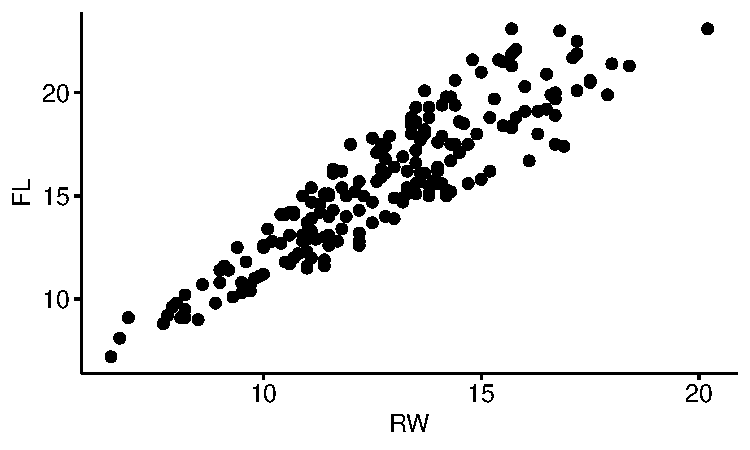
\includegraphics{bookdown-demo_files/figure-latex/unnamed-chunk-40-1.pdf}

\textbf{End optional section}

\begin{center}\rule{0.5\linewidth}{\linethickness}\end{center}

\section{Challenge}\label{challenge}

An another add-on to ggplot2 is cowplot, which stands for
\href{https://cran.r-project.org/web/packages/cowplot/vignettes/introduction.html}{``Claus
O. Wilke Plot''}. Download cowplot from CRAN using either the
point-and-click method or \textbf{install.packages}, and then load it
using \textbf{library}. Then run the following R code, which should make
the plot below.

\textbf{Note that ``FL'' and ``RW'' are NOT in quotation marks as they
are for ggscatter()!}

\begin{Shaded}
\begin{Highlighting}[]
\KeywordTok{qplot}\NormalTok{(}\DataTypeTok{data =}\NormalTok{ crabs, }\DataTypeTok{y =}\NormalTok{ FL, }\DataTypeTok{x =}\NormalTok{ RW) }\CommentTok{#no quotes!}
\end{Highlighting}
\end{Shaded}

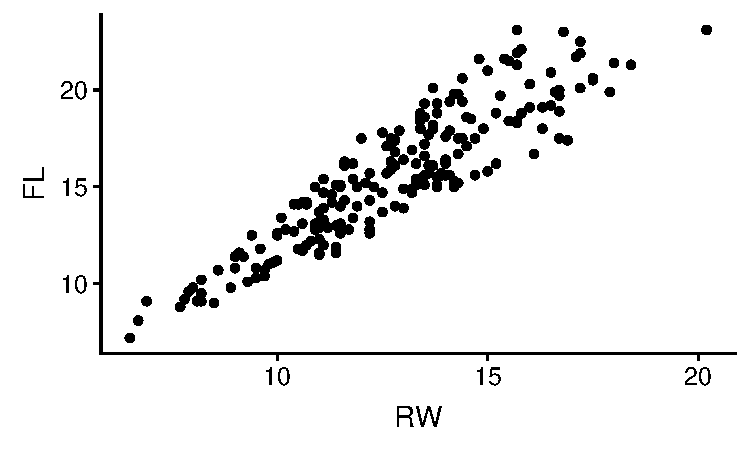
\includegraphics{bookdown-demo_files/figure-latex/unnamed-chunk-42-1.pdf}

\chapter{Loading data into R from a
package}\label{loading-data-into-r-from-a-package}

\textbf{Nathan Brouwer, Phd}\\
brouwern at gmail.com\\
\url{https://github.com/brouwern}\\
Twitter: lobrowR

\section{Introduction}\label{introduction-1}

Working in R is all about working with data. There are many ways to get
data into R, and RStudio has some helpful tools for this process. In
this exercise we'll go over the common ways that data get's brought into
R and how to download external packages to get datasets and functions.
These include data

\begin{itemize}
\tightlist
\item
  pre-loaded in R
\item
  loaded in R ``packages''
\item
  typed into a script
\item
  loaded from a spreadsheet using RStudio's data import tools
\item
  loaded from a spreadsheet using just R code
\end{itemize}

While discussing these various routes for data to get into R we'll also
talk a bit about how R works with data and learn data related vocab.

\subsection{Functions}\label{functions}

\begin{itemize}
\tightlist
\item
  head(), tail()
\item
  summary()
\end{itemize}

\subsection{Datsets}\label{datsets}

\begin{itemize}
\tightlist
\item
  datasets::iris
\end{itemize}

\subsection{Packages}\label{packages-1}

\subsection{Key terms}\label{key-terms}

\begin{itemize}
\tightlist
\item
  package
\item
  dataframe
\end{itemize}

\section{Data pre-loaded in R}\label{data-pre-loaded-in-r}

R comes with a number of datasets ready to use. A famous dataset
frequently used in statistics is a set of measurements made on three
species of irises and used to demonstrate some statistical principles by
geneticist and statistician R.A. Fisher.

We can put the iris dataset into R's working memory using the data()
command

\begin{Shaded}
\begin{Highlighting}[]
\KeywordTok{data}\NormalTok{(iris)}
\end{Highlighting}
\end{Shaded}

We can see these data simply by type the word ``iris'' in the console
and pressing enter. The dataset is too big for the screen probably and
you'll just see a bunch of numbers flash by. You can get just a glimpse
of the data by using the head() command, which will show you the first
six or so rows of data.

\begin{Shaded}
\begin{Highlighting}[]
\KeywordTok{head}\NormalTok{(iris)}
\end{Highlighting}
\end{Shaded}

\begin{verbatim}
##   Sepal.Length Sepal.Width Petal.Length Petal.Width Species
## 1          5.1         3.5          1.4         0.2  setosa
## 2          4.9         3.0          1.4         0.2  setosa
## 3          4.7         3.2          1.3         0.2  setosa
## 4          4.6         3.1          1.5         0.2  setosa
## 5          5.0         3.6          1.4         0.2  setosa
## 6          5.4         3.9          1.7         0.4  setosa
\end{verbatim}

(You can all use the tail() command to see the last 6 rows if you want.)

We can see that there are five rows of data. Three contain information
about the length and width of the parts of the flower (Sepals and
Petals) and the last holds the names of the species.

We can get a sense for these numbers by using the summary() command on
the data, which will give us the mean and other summary statistics

\begin{Shaded}
\begin{Highlighting}[]
\KeywordTok{summary}\NormalTok{(iris)}
\end{Highlighting}
\end{Shaded}

\begin{verbatim}
##   Sepal.Length    Sepal.Width     Petal.Length    Petal.Width   
##  Min.   :4.300   Min.   :2.000   Min.   :1.000   Min.   :0.100  
##  1st Qu.:5.100   1st Qu.:2.800   1st Qu.:1.600   1st Qu.:0.300  
##  Median :5.800   Median :3.000   Median :4.350   Median :1.300  
##  Mean   :5.843   Mean   :3.057   Mean   :3.758   Mean   :1.199  
##  3rd Qu.:6.400   3rd Qu.:3.300   3rd Qu.:5.100   3rd Qu.:1.800  
##  Max.   :7.900   Max.   :4.400   Max.   :6.900   Max.   :2.500  
##        Species  
##  setosa    :50  
##  versicolor:50  
##  virginica :50  
##                 
##                 
## 
\end{verbatim}

Note that the last column doesn't contain numbers but rather names, so R
counts up how many of each species name there is.

If we want to be reminded of the names of each column we can use the
names() function

\begin{Shaded}
\begin{Highlighting}[]
\KeywordTok{names}\NormalTok{(iris)}
\end{Highlighting}
\end{Shaded}

\begin{verbatim}
## [1] "Sepal.Length" "Sepal.Width"  "Petal.Length" "Petal.Width" 
## [5] "Species"
\end{verbatim}

Looking at R data in the console isn't always very easy, so one thing
you can do is use the View() command. This will bring up the data in a
spreadsheet like viewer as a new tab in the script editor, similar to
this.

\begin{Shaded}
\begin{Highlighting}[]
\NormalTok{pander}\OperatorTok{::}\KeywordTok{pander}\NormalTok{(iris[}\DecValTok{1}\OperatorTok{:}\DecValTok{10}\NormalTok{,])}
\end{Highlighting}
\end{Shaded}

\begin{longtable}[]{@{}ccccc@{}}
\toprule
\begin{minipage}[b]{0.18\columnwidth}\centering\strut
Sepal.Length\strut
\end{minipage} & \begin{minipage}[b]{0.17\columnwidth}\centering\strut
Sepal.Width\strut
\end{minipage} & \begin{minipage}[b]{0.18\columnwidth}\centering\strut
Petal.Length\strut
\end{minipage} & \begin{minipage}[b]{0.17\columnwidth}\centering\strut
Petal.Width\strut
\end{minipage} & \begin{minipage}[b]{0.11\columnwidth}\centering\strut
Species\strut
\end{minipage}\tabularnewline
\midrule
\endhead
\begin{minipage}[t]{0.18\columnwidth}\centering\strut
5.1\strut
\end{minipage} & \begin{minipage}[t]{0.17\columnwidth}\centering\strut
3.5\strut
\end{minipage} & \begin{minipage}[t]{0.18\columnwidth}\centering\strut
1.4\strut
\end{minipage} & \begin{minipage}[t]{0.17\columnwidth}\centering\strut
0.2\strut
\end{minipage} & \begin{minipage}[t]{0.11\columnwidth}\centering\strut
setosa\strut
\end{minipage}\tabularnewline
\begin{minipage}[t]{0.18\columnwidth}\centering\strut
4.9\strut
\end{minipage} & \begin{minipage}[t]{0.17\columnwidth}\centering\strut
3\strut
\end{minipage} & \begin{minipage}[t]{0.18\columnwidth}\centering\strut
1.4\strut
\end{minipage} & \begin{minipage}[t]{0.17\columnwidth}\centering\strut
0.2\strut
\end{minipage} & \begin{minipage}[t]{0.11\columnwidth}\centering\strut
setosa\strut
\end{minipage}\tabularnewline
\begin{minipage}[t]{0.18\columnwidth}\centering\strut
4.7\strut
\end{minipage} & \begin{minipage}[t]{0.17\columnwidth}\centering\strut
3.2\strut
\end{minipage} & \begin{minipage}[t]{0.18\columnwidth}\centering\strut
1.3\strut
\end{minipage} & \begin{minipage}[t]{0.17\columnwidth}\centering\strut
0.2\strut
\end{minipage} & \begin{minipage}[t]{0.11\columnwidth}\centering\strut
setosa\strut
\end{minipage}\tabularnewline
\begin{minipage}[t]{0.18\columnwidth}\centering\strut
4.6\strut
\end{minipage} & \begin{minipage}[t]{0.17\columnwidth}\centering\strut
3.1\strut
\end{minipage} & \begin{minipage}[t]{0.18\columnwidth}\centering\strut
1.5\strut
\end{minipage} & \begin{minipage}[t]{0.17\columnwidth}\centering\strut
0.2\strut
\end{minipage} & \begin{minipage}[t]{0.11\columnwidth}\centering\strut
setosa\strut
\end{minipage}\tabularnewline
\begin{minipage}[t]{0.18\columnwidth}\centering\strut
5\strut
\end{minipage} & \begin{minipage}[t]{0.17\columnwidth}\centering\strut
3.6\strut
\end{minipage} & \begin{minipage}[t]{0.18\columnwidth}\centering\strut
1.4\strut
\end{minipage} & \begin{minipage}[t]{0.17\columnwidth}\centering\strut
0.2\strut
\end{minipage} & \begin{minipage}[t]{0.11\columnwidth}\centering\strut
setosa\strut
\end{minipage}\tabularnewline
\begin{minipage}[t]{0.18\columnwidth}\centering\strut
5.4\strut
\end{minipage} & \begin{minipage}[t]{0.17\columnwidth}\centering\strut
3.9\strut
\end{minipage} & \begin{minipage}[t]{0.18\columnwidth}\centering\strut
1.7\strut
\end{minipage} & \begin{minipage}[t]{0.17\columnwidth}\centering\strut
0.4\strut
\end{minipage} & \begin{minipage}[t]{0.11\columnwidth}\centering\strut
setosa\strut
\end{minipage}\tabularnewline
\begin{minipage}[t]{0.18\columnwidth}\centering\strut
4.6\strut
\end{minipage} & \begin{minipage}[t]{0.17\columnwidth}\centering\strut
3.4\strut
\end{minipage} & \begin{minipage}[t]{0.18\columnwidth}\centering\strut
1.4\strut
\end{minipage} & \begin{minipage}[t]{0.17\columnwidth}\centering\strut
0.3\strut
\end{minipage} & \begin{minipage}[t]{0.11\columnwidth}\centering\strut
setosa\strut
\end{minipage}\tabularnewline
\begin{minipage}[t]{0.18\columnwidth}\centering\strut
5\strut
\end{minipage} & \begin{minipage}[t]{0.17\columnwidth}\centering\strut
3.4\strut
\end{minipage} & \begin{minipage}[t]{0.18\columnwidth}\centering\strut
1.5\strut
\end{minipage} & \begin{minipage}[t]{0.17\columnwidth}\centering\strut
0.2\strut
\end{minipage} & \begin{minipage}[t]{0.11\columnwidth}\centering\strut
setosa\strut
\end{minipage}\tabularnewline
\begin{minipage}[t]{0.18\columnwidth}\centering\strut
4.4\strut
\end{minipage} & \begin{minipage}[t]{0.17\columnwidth}\centering\strut
2.9\strut
\end{minipage} & \begin{minipage}[t]{0.18\columnwidth}\centering\strut
1.4\strut
\end{minipage} & \begin{minipage}[t]{0.17\columnwidth}\centering\strut
0.2\strut
\end{minipage} & \begin{minipage}[t]{0.11\columnwidth}\centering\strut
setosa\strut
\end{minipage}\tabularnewline
\begin{minipage}[t]{0.18\columnwidth}\centering\strut
4.9\strut
\end{minipage} & \begin{minipage}[t]{0.17\columnwidth}\centering\strut
3.1\strut
\end{minipage} & \begin{minipage}[t]{0.18\columnwidth}\centering\strut
1.5\strut
\end{minipage} & \begin{minipage}[t]{0.17\columnwidth}\centering\strut
0.1\strut
\end{minipage} & \begin{minipage}[t]{0.11\columnwidth}\centering\strut
setosa\strut
\end{minipage}\tabularnewline
\bottomrule
\end{longtable}

Note, however, that unlike a spreadsheet you cannot edit the data.

If you want to know more about a package, you can look at its help file,
eg ``?iris.'' These will often give you a fair bit of detail about what
each column means, where the data are from, and may even have examples R
functions applied to the data (though these can be rather obtuse, as is
the case for the iris data).

\subsection{Preview: Plotting boxplots}\label{preview-plotting-boxplots}

Plotting will be covered in depth in a subsequent exercise, but here's a
glimpse of how we plot things in R:

\begin{Shaded}
\begin{Highlighting}[]
\KeywordTok{plot}\NormalTok{(Petal.Length }\OperatorTok{~}\StringTok{ }\NormalTok{Species, }\DataTypeTok{data =}\NormalTok{ iris)}
\end{Highlighting}
\end{Shaded}

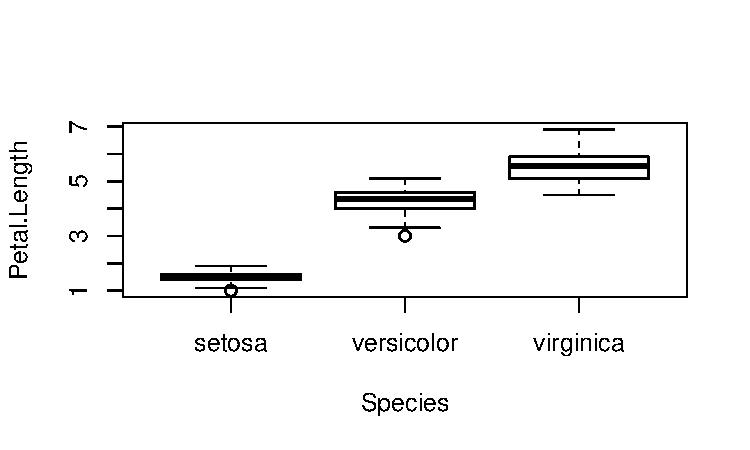
\includegraphics{bookdown-demo_files/figure-latex/unnamed-chunk-49-1.pdf}

This code creates a series of \textbf{boxplots} of the petal lengths of
each species of flower.

\section{Loading data from R
packages}\label{loading-data-from-r-packages}

Base R however is surrounded by a universe of extensions built by
statistician, programmers, academics and businesses that use R for
analyses. Some of these are fairly standard and are downloaded along
with base R and just need to be explicitly installed. Other have to be
downloaded from the internet and installed. Most packages contain data
in order to demonstrate what they do.

\subsection{Loading a package contained in base
R}\label{loading-a-package-contained-in-base-r}

One package that is automatically downloaded but not automatically
\emph{installed} with base R is the ``MASS'' package, which stands for
``Modern Applied Statistics in R''; S is the software that preceded R.
We can install this package and make it functionally using the library()
command

\begin{Shaded}
\begin{Highlighting}[]
\KeywordTok{library}\NormalTok{(MASS)}
\end{Highlighting}
\end{Shaded}

The MASS package has a biological dataset called ``crabs'' that you can
put into working memory using data(crabs). We can then look at it using
head(),View(), tail(), summary(), etc. We can find out more about the
dataset using the help file, accessed via ?crabs

\textbf{Question} 1.What does the ``FL'' column mean in the crabs
dataset? 1.What is the mean of the FL column?

\subsection{Preview: Plotting scatter
plot}\label{preview-plotting-scatter-plot}

We can plot the relationship between the FL and RW variables using a
scatter plot.

\begin{Shaded}
\begin{Highlighting}[]
\KeywordTok{plot}\NormalTok{(FL }\OperatorTok{~}\StringTok{ }\NormalTok{RW, }\DataTypeTok{data =}\NormalTok{ crabs)}
\end{Highlighting}
\end{Shaded}

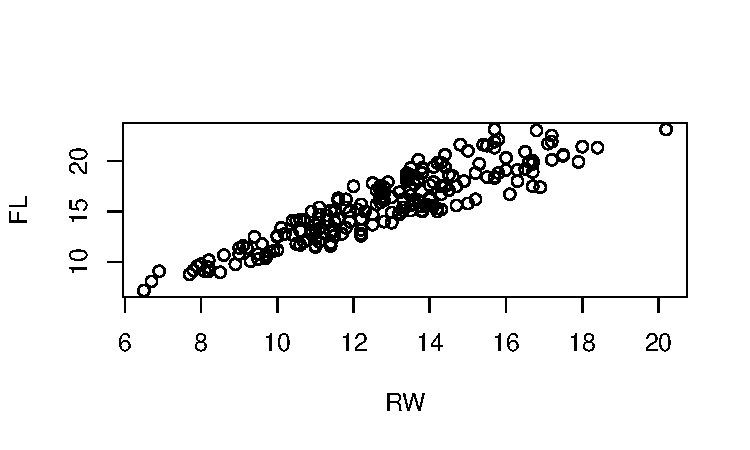
\includegraphics{bookdown-demo_files/figure-latex/unnamed-chunk-51-1.pdf}

\section{Learning about data in R}\label{learning-about-data-in-r}

When data is being worked with in R, it lives in a place called the
\textbf{workspace.} The workspace is not immediately transparent to you
while working in R. It lives behind the scenes in what is essentially
R's working memory. We can see what's on R's mind using the ls() command

\begin{Shaded}
\begin{Highlighting}[]
\KeywordTok{ls}\NormalTok{()}
\end{Highlighting}
\end{Shaded}

\begin{verbatim}
## [1] "crabs" "iris"  "x"
\end{verbatim}

We can see our two datasets that we loaded using the data() command.

We can add new things to the work space using an R command like this

\begin{Shaded}
\begin{Highlighting}[]
\NormalTok{my.mean <-}\StringTok{ }\KeywordTok{mean}\NormalTok{(}\KeywordTok{c}\NormalTok{(}\DecValTok{1}\NormalTok{,}\DecValTok{2}\NormalTok{,}\DecValTok{2}\NormalTok{))}
\end{Highlighting}
\end{Shaded}

Where ``\textless{}-'' is called the \textbf{assignment operator}. This
function \textbf{assigns} the output of an R command or R function to an
\textbf{R object} in R's working memory, the workspace.

We can check again what's on R's mind using a command ls(), which stands
for ``list''

\begin{Shaded}
\begin{Highlighting}[]
\KeywordTok{ls}\NormalTok{()}
\end{Highlighting}
\end{Shaded}

\begin{verbatim}
## [1] "crabs"   "iris"    "my.mean" "x"
\end{verbatim}

We can see that we added my.mean. We can see what my.mean is by typing
its name in to the console

\begin{Shaded}
\begin{Highlighting}[]
\NormalTok{my.mean}
\end{Highlighting}
\end{Shaded}

\begin{verbatim}
## [1] 1.666667
\end{verbatim}

We can also learn more about is using the is() command

\begin{Shaded}
\begin{Highlighting}[]
\KeywordTok{is}\NormalTok{(my.mean)}
\end{Highlighting}
\end{Shaded}

\begin{verbatim}
## [1] "numeric" "vector"
\end{verbatim}

Here we get a big of R lingo: R tells use ``numeric'', which means it
contain numeric data (numbers), and ``vector'', which is one of several
types of R object

R objects can be just about anything. We can assign letter to an R
object like this

\begin{Shaded}
\begin{Highlighting}[]
\NormalTok{my.abc <-}\StringTok{ }\KeywordTok{c}\NormalTok{(}\StringTok{"a"}\NormalTok{,}\StringTok{"b"}\NormalTok{,}\StringTok{"c"}\NormalTok{)}
\end{Highlighting}
\end{Shaded}

Note that we have the letter each surrounded by quotes, and all 3 of
them within c(\ldots{})

If you call up ``my.abc'' from the console, you will get back the three
letter. Now see what is(my.abc) says

\begin{Shaded}
\begin{Highlighting}[]
\KeywordTok{is}\NormalTok{(my.abc)}
\end{Highlighting}
\end{Shaded}

\begin{verbatim}
## [1] "character"           "vector"              "data.frameRowLabels"
## [4] "SuperClassMethod"
\end{verbatim}

There's a lot that comes out, but the first one says ``character'',
indicating that yo have \textbf{character data} - data made up of text.

If you type ls() again what happens?

\begin{Shaded}
\begin{Highlighting}[]
\KeywordTok{ls}\NormalTok{()}
\end{Highlighting}
\end{Shaded}

\begin{verbatim}
## [1] "crabs"   "iris"    "my.abc"  "my.mean" "x"
\end{verbatim}

We now see both of our R objects and the two datasets.

If we call is() on one of the dataset what do we is?

\begin{Shaded}
\begin{Highlighting}[]
\KeywordTok{is}\NormalTok{(crabs)}
\end{Highlighting}
\end{Shaded}

\begin{verbatim}
## [1] "data.frame" "list"       "oldClass"   "vector"
\end{verbatim}

Several things get spit out, but the first one is important:
``data.frame'' Dataframes are fundamental units of analysis in R. Most
of the data you will load into R and work within R will be in a
dataframe.

Another function that tells about something in the the workspace is
str(), which stands for structure. It provides info about what types of
variables are in each column, and provides some sample output similar to
head(), but oriented differently.

\begin{Shaded}
\begin{Highlighting}[]
\KeywordTok{str}\NormalTok{(crabs)}
\end{Highlighting}
\end{Shaded}

\begin{verbatim}
## 'data.frame':    200 obs. of  8 variables:
##  $ sp   : Factor w/ 2 levels "B","O": 1 1 1 1 1 1 1 1 1 1 ...
##  $ sex  : Factor w/ 2 levels "F","M": 2 2 2 2 2 2 2 2 2 2 ...
##  $ index: int  1 2 3 4 5 6 7 8 9 10 ...
##  $ FL   : num  8.1 8.8 9.2 9.6 9.8 10.8 11.1 11.6 11.8 11.8 ...
##  $ RW   : num  6.7 7.7 7.8 7.9 8 9 9.9 9.1 9.6 10.5 ...
##  $ CL   : num  16.1 18.1 19 20.1 20.3 23 23.8 24.5 24.2 25.2 ...
##  $ CW   : num  19 20.8 22.4 23.1 23 26.5 27.1 28.4 27.8 29.3 ...
##  $ BD   : num  7 7.4 7.7 8.2 8.2 9.8 9.8 10.4 9.7 10.3 ...
\end{verbatim}

Note that the variables ``sp'', which stands for ``Species'', and
``sex'' are followed by the word ``Factor.'' A \textbf{factor variable}
is something that is or is summarized as discrete categories. For the
species factor, there are two levels: the ``B'' species and the ``O''
species.

\section{Load data from an external R
package}\label{load-data-from-an-external-r-package-1}

Many packages have to be explicitly downloaded and installed in order to
use their functions and datasets. Note that this is a \textbf{two step
process}: 1. Download package from internet 1. Explicitly tell R to load
it

\subsection{Step 1: Downloading
packages}\label{step-1-downloading-packages}

There are a number of ways to install packages. One of the easiest is to
use install.packages(). Note that it might be better to call this
``download.packages'' since after you install it, you also have to load
it!

Well download a package used for plotting called ggplot2, which stands
for ``Grammar of graphics''

\begin{Shaded}
\begin{Highlighting}[]
\KeywordTok{install.packages}\NormalTok{(}\StringTok{"ggplot2"}\NormalTok{)}
\end{Highlighting}
\end{Shaded}

Often when you download a package you'll see a fair bit of red text.
Usually there's nothing of interest hear, but sometimes you need to read
over it for hints about why something didn't work.

\subsection{Step 2: Explicitly loading a
package}\label{step-2-explicitly-loading-a-package}

The install.packages() functions just saves the package software to R;
now you need to tell R ``I want to work with the package''. This is done
using the library() function. (Its called library because another name
for packages is libraries)

\begin{Shaded}
\begin{Highlighting}[]
\KeywordTok{library}\NormalTok{(ggplot2)}
\end{Highlighting}
\end{Shaded}

ggplot2 has a dataset called ``msleep'' which has information on the
relationship between the typical size of a species and its brain weight,
among other things

We load the data actively into R's memory using data(), and can look at
the column names using names()

\begin{Shaded}
\begin{Highlighting}[]
\KeywordTok{data}\NormalTok{(msleep)}
\KeywordTok{names}\NormalTok{(msleep)}
\end{Highlighting}
\end{Shaded}

\begin{verbatim}
##  [1] "name"         "genus"        "vore"         "order"       
##  [5] "conservation" "sleep_total"  "sleep_rem"    "sleep_cycle" 
##  [9] "awake"        "brainwt"      "bodywt"
\end{verbatim}

We can now explore this data set as before using summary(), str(), etc.

Another useful command when you are working with a new dataset is dim().
This tells you the dimension of the dataframe

\begin{Shaded}
\begin{Highlighting}[]
\KeywordTok{dim}\NormalTok{(msleep)}
\end{Highlighting}
\end{Shaded}

\begin{verbatim}
## [1] 83 11
\end{verbatim}

\subsection{Preview: plotting with
ggplot2}\label{preview-plotting-with-ggplot2}

ggplot2 is a powerful plotting tool that has become standard among
scientists, data scientists, and even journalists. Here's a quick way to
make a plot in ggplot2 using its qplot() function (qplot = quick plot,
not to be confused with qqplot). Note that the qplot() function only
works if you have ggplot2 downloaded and installed.

A powerful aspect of ggplot is the fact that it can easily be used to
modify plots. Here, we use the \textbf{arguement} ``color ='' to color
code the data points based on their IUCN red list status.

\begin{Shaded}
\begin{Highlighting}[]
\KeywordTok{qplot}\NormalTok{(}\DataTypeTok{y =}\NormalTok{ brainwt, }\DataTypeTok{x =}\NormalTok{ bodywt, }\DataTypeTok{data =}\NormalTok{ msleep, }\DataTypeTok{color =}\NormalTok{ conservation)}
\end{Highlighting}
\end{Shaded}

\begin{verbatim}
## Warning: Removed 27 rows containing missing values (geom_point).
\end{verbatim}

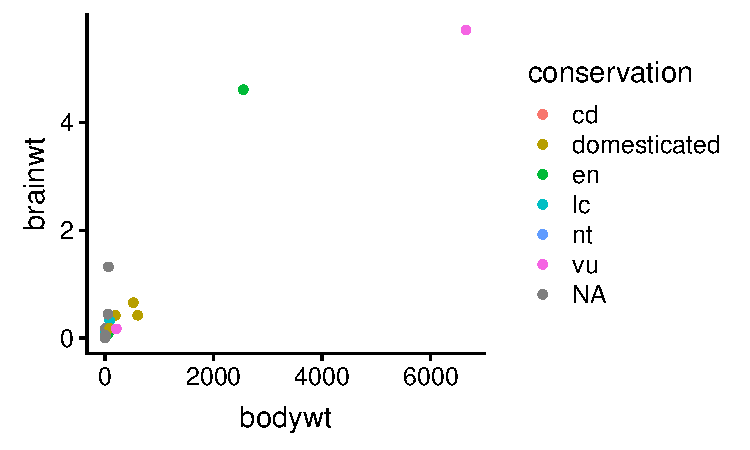
\includegraphics{bookdown-demo_files/figure-latex/unnamed-chunk-66-1.pdf}

The animals in this data vary in size from mice to elephants and so a
lot of the data points are scrunched together. A trick to make this
easier to see is to take the log of the brainwt and bodywt variable. In
R, we can do this on the fly like this using the log() command

\begin{Shaded}
\begin{Highlighting}[]
\KeywordTok{qplot}\NormalTok{(}\DataTypeTok{y =} \KeywordTok{log}\NormalTok{(brainwt), }\DataTypeTok{x =} \KeywordTok{log}\NormalTok{(bodywt), }\DataTypeTok{data =}\NormalTok{ msleep, }\DataTypeTok{color =}\NormalTok{ conservation)}
\end{Highlighting}
\end{Shaded}

\begin{verbatim}
## Warning: Removed 27 rows containing missing values (geom_point).
\end{verbatim}

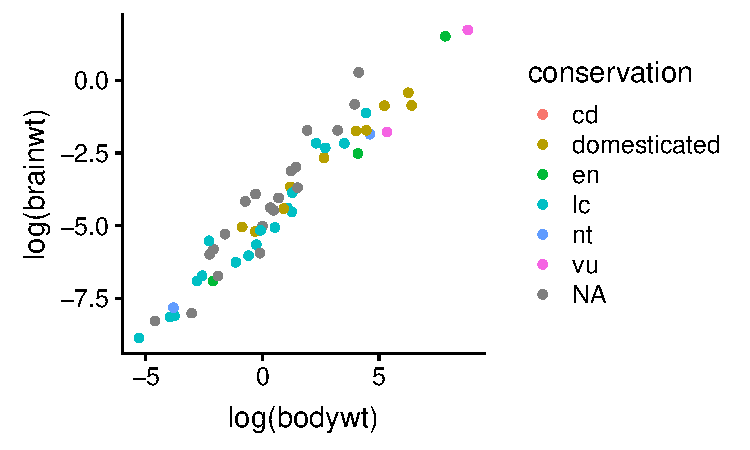
\includegraphics{bookdown-demo_files/figure-latex/unnamed-chunk-67-1.pdf}

\section{Loading data from an R
script}\label{loading-data-from-an-r-script}

So far we have only looked at dataset that are already formatted into
\textbf{dataframe} by somebody for us. Now we want to look at how to set
up datasets ourselves. When datasets are small its possible to enter
them more or less directly into R by typing out all of the numbers in a
script. This only works well for when datasets are small; even when
datasets are small its best to keep them separate from your R code in a
spreadsheet file. However, its useful to know how to load data this way;
even when an exercise in this book loads data from a package or
spreadsheet I will also often include the code to load it directly just
in case there is an issue with download the package or file.

\subsection{The eagles have landed - in your R
workspace}\label{the-eagles-have-landed---in-your-r-workspace}

In a subsequent exercise we will practice using data on the number of
eagles in Pennsylvania and other states in the USA. We can load this
data into R by making R objects, and then turning these objects into a
dataframe.

\subsubsection{Step one: Build R
objects}\label{step-one-build-r-objects}

First, we'll use the assignment operator (``\textless{}-'') to create an
R object called ``year'' that lists the years from 1980 through 2015 for
which the number breeding pairs of eagles in Pennsylvania, USA, is
known.

\begin{Shaded}
\begin{Highlighting}[]
\NormalTok{year <-}\StringTok{ }\KeywordTok{c}\NormalTok{(}\DecValTok{1980}\NormalTok{,}\DecValTok{1981}\NormalTok{,}\DecValTok{1982}\NormalTok{,}\DecValTok{1983}\NormalTok{,}\DecValTok{1984}\NormalTok{,}\DecValTok{1985}\NormalTok{,}\DecValTok{1986}\NormalTok{,}\DecValTok{1987}\NormalTok{,}\DecValTok{1988}\NormalTok{,}\DecValTok{1989}\NormalTok{,}
          \DecValTok{1990}\NormalTok{,}\DecValTok{1991}\NormalTok{,}\DecValTok{1992}\NormalTok{,}\DecValTok{1993}\NormalTok{,}\DecValTok{1994}\NormalTok{,}\DecValTok{1995}\NormalTok{,}\DecValTok{1996}\NormalTok{,}\DecValTok{1997}\NormalTok{,}\DecValTok{1998}\NormalTok{,}\DecValTok{1999}\NormalTok{,}
          \DecValTok{2000}\NormalTok{,}\DecValTok{2001}\NormalTok{,}\DecValTok{2002}\NormalTok{,}\DecValTok{2003}\NormalTok{,}\DecValTok{2004}\NormalTok{,}\DecValTok{2005}\NormalTok{,}\DecValTok{2006}\NormalTok{,}\DecValTok{2007}\NormalTok{,}\DecValTok{2008}\NormalTok{,}\DecValTok{2009}\NormalTok{,}
          \DecValTok{2010}\NormalTok{,}\DecValTok{2011}\NormalTok{,}\DecValTok{2012}\NormalTok{,}\DecValTok{2013}\NormalTok{,}\DecValTok{2014}\NormalTok{,}\DecValTok{2015}\NormalTok{,}\DecValTok{2016}\NormalTok{)}
\end{Highlighting}
\end{Shaded}

A quick trick to do this much fast is

\begin{Shaded}
\begin{Highlighting}[]
\NormalTok{year <-}\StringTok{ }\KeywordTok{c}\NormalTok{(}\DecValTok{1980}\OperatorTok{:}\DecValTok{2016}\NormalTok{)}
\end{Highlighting}
\end{Shaded}

Second, we'll create an object called ``eagles'' with the number of
breeding pairs (male and females paired up for making baby eagles)
recorded each year. Note that most years in the 1980s are skipped
because there is not data available. When data are missing we use NA.
(Note that this is just NA, with not quotes around it).

\begin{Shaded}
\begin{Highlighting}[]
\NormalTok{eagles <-}\StringTok{  }\KeywordTok{c}\NormalTok{(}\DecValTok{3}\NormalTok{, }\OtherTok{NA}\NormalTok{, }\OtherTok{NA}\NormalTok{, }\OtherTok{NA}\NormalTok{, }\OtherTok{NA}\NormalTok{, }\OtherTok{NA}\NormalTok{, }\OtherTok{NA}\NormalTok{,}\OtherTok{NA}\NormalTok{,}\OtherTok{NA}\NormalTok{,}\OtherTok{NA}\NormalTok{,}
             \DecValTok{7}\NormalTok{,  }\DecValTok{9}\NormalTok{, }\DecValTok{15}\NormalTok{, }\DecValTok{17}\NormalTok{, }\DecValTok{19}\NormalTok{, }\DecValTok{20}\NormalTok{, }\DecValTok{20}\NormalTok{,}\DecValTok{23}\NormalTok{,}\DecValTok{29}\NormalTok{,}\DecValTok{43}\NormalTok{,}
             \DecValTok{51}\NormalTok{,}\DecValTok{55}\NormalTok{, }\DecValTok{64}\NormalTok{, }\DecValTok{69}\NormalTok{, }\OtherTok{NA}\NormalTok{, }\DecValTok{96}\NormalTok{,}\DecValTok{100}\NormalTok{,}\OtherTok{NA}\NormalTok{,}\OtherTok{NA}\NormalTok{,}\OtherTok{NA}\NormalTok{,}
             \OtherTok{NA}\NormalTok{,}\OtherTok{NA}\NormalTok{, }\OtherTok{NA}\NormalTok{, }\OtherTok{NA}\NormalTok{,}\DecValTok{252}\NormalTok{,}\DecValTok{277}\NormalTok{, }\OtherTok{NA}\NormalTok{)}
\end{Highlighting}
\end{Shaded}

\subsubsection{Step two: Build
dataframe}\label{step-two-build-dataframe}

We can then turn these two separate R objects into a dataframe

\begin{Shaded}
\begin{Highlighting}[]
\NormalTok{eagle.df <-}\KeywordTok{data.frame}\NormalTok{(year, eagles)}
\end{Highlighting}
\end{Shaded}

\subsection{Looking at the eagle data}\label{looking-at-the-eagle-data}

We can check that we have this R object by using the \textbf{ls()}
command.

\begin{Shaded}
\begin{Highlighting}[]
\KeywordTok{ls}\NormalTok{()}
\end{Highlighting}
\end{Shaded}

\begin{verbatim}
## [1] "crabs"    "eagle.df" "eagles"   "iris"     "msleep"   "my.abc"  
## [7] "my.mean"  "x"        "year"
\end{verbatim}

And we can confirm that its a dataframe using \textbf{is()}

\begin{Shaded}
\begin{Highlighting}[]
\KeywordTok{is}\NormalTok{(eagle.df)}
\end{Highlighting}
\end{Shaded}

\begin{verbatim}
## [1] "data.frame" "list"       "oldClass"   "vector"
\end{verbatim}

\textbf{summary()} will give us basic info on PA's eagles

\begin{Shaded}
\begin{Highlighting}[]
\KeywordTok{summary}\NormalTok{(eagle.df)}
\end{Highlighting}
\end{Shaded}

\begin{verbatim}
##       year          eagles      
##  Min.   :1980   Min.   :  3.00  
##  1st Qu.:1989   1st Qu.: 18.00  
##  Median :1998   Median : 29.00  
##  Mean   :1998   Mean   : 61.53  
##  3rd Qu.:2007   3rd Qu.: 66.50  
##  Max.   :2016   Max.   :277.00  
##                 NA's   :18
\end{verbatim}

Note that in the ``eagles'' columns it tells you the number of NAs
(missing values). The summary() readout quickly tells us that the eagle
population has changed dramatically.

\subsubsection{Preview: Plotting the Eagle
D}\label{preview-plotting-the-eagle-d}

We can plot the data in ggplot2 using qplot(). However, there is an
excellent package that adds additional functionality to ggplot called
ggpubr. This is fairly common in R: you have packages that add functions
to R, and packages that add functions to other packages.

We can install ggpubr using install.packages(). Note that the name of
the package, ggpubr, is in quotes.

\begin{Shaded}
\begin{Highlighting}[]
\KeywordTok{install.packages}\NormalTok{(}\StringTok{"ggpubr"}\NormalTok{)}
\end{Highlighting}
\end{Shaded}

ggpubr requires \emph{another package}, magrittr, which R tells you
about in red text. When a package requires another package, its called a
\textbf{dependency} because one package relies on another. ggpubr has
magrittr as a dependency; ggpubr modifies ggplot2, so ggpubr has ggplot2
as a dependency.

Occasionally you might try to load a package and it won't automatically
install or download the dependency, usually because its not yet
downloaded. If this happens with magrittr we would just have to download
it using ``install.packages(''magrittr``)''.

Once we have ggpubr loaded we can plot the eagle data using the handy
function \textbf{ggscatter()}

\begin{Shaded}
\begin{Highlighting}[]
\KeywordTok{ggscatter}\NormalTok{(}\DataTypeTok{dat =}\NormalTok{ eagle.df, }\DataTypeTok{y =} \StringTok{"eagles"}\NormalTok{, }\DataTypeTok{x=} \StringTok{"year"}\NormalTok{)}
\end{Highlighting}
\end{Shaded}

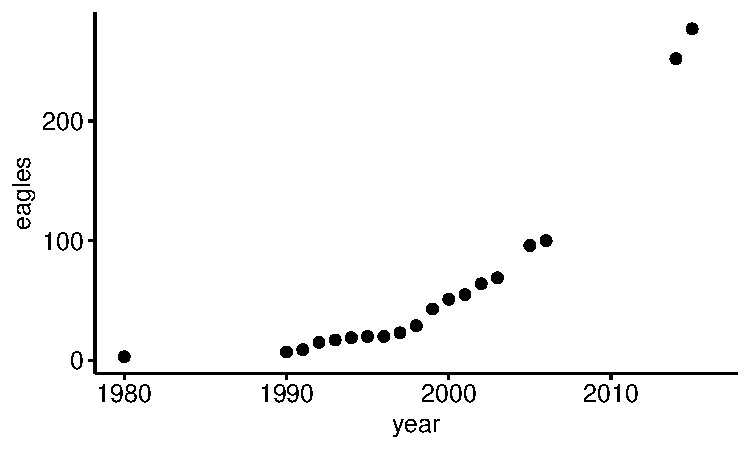
\includegraphics{bookdown-demo_files/figure-latex/unnamed-chunk-77-1.pdf}

\section{Challenge}\label{challenge-1}

We can add a \textbf{smoother} to the plot by addin add = ``loess''.

\begin{verbatim}
## Warning: Removed 18 rows containing non-finite values (stat_smooth).
\end{verbatim}

\begin{verbatim}
## Warning: Removed 18 rows containing missing values (geom_point).
\end{verbatim}

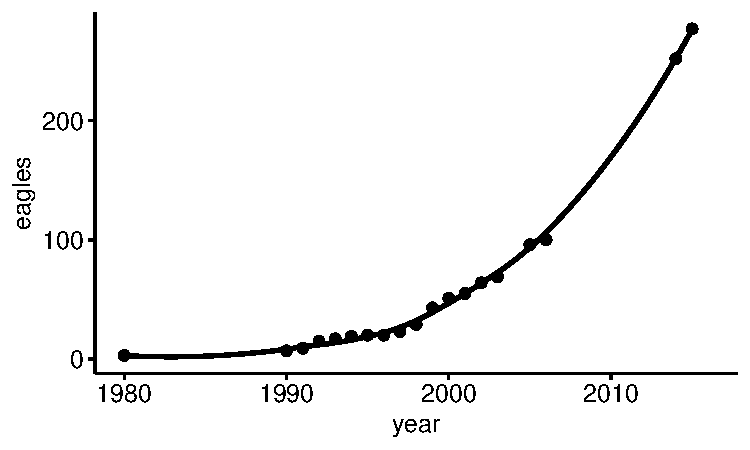
\includegraphics{bookdown-demo_files/figure-latex/unnamed-chunk-78-1.pdf}

\chapter{Loading packages \& data from
GitHub}\label{loading-packages-data-from-github}

\textbf{Nathan Brouwer, Phd}\\
\href{mailto:brouwern@gmail.com}{\nolinkurl{brouwern@gmail.com}}\\
\url{https://github.com/brouwern}\\
\citet{lobrowR}

\section{Introduction}\label{introduction-2}

\textbf{GitHub} is an online platform for hosting and sharing code. More
formally it is called a \textbf{software repository}. It is very popular
with software developers, especially those creating open-source
applications, and has also been adopted whole-hearted by many data
scientists and data analysts.

GitHub has many features and uses. One of the most basic ones is to use
GitHub like Dropbox to R backup copies of code on GitHub. GitHub also
can act like a kind of web server to host websites, online books like
this one, and provide access to open source software. Many people
working on R packages use GitHub to host their package while its being
developed or expanded. When a package is finished, it often is then
submitted to CRAN, and the version on GitHub is used as the
\textbf{developement version} where new features are being developed and
tested.

You can access packages on GitHub to get the newest version before
something has been submitted to CRAN, or packages that haven't or maybe
will never end up on CRAN. This book relies on a package I've written
called \textbf{wildlifeR} for datasets and some functions. In this short
exercise we'll download a package from CRAN we need to interact with
GitHub, and then download wildlifeR. We'll also go to the wildlifeR
website to learn more about the package.

\subsection{Learning objectives}\label{learning-objectives-1}

\subsection{Learning goals}\label{learning-goals-1}

\subsection{Functions \& Arguements}\label{functions-arguements-1}

\begin{itemize}
\tightlist
\item
  library
\item
  devtools::install\_github
\item
  scatter.smooth
\item
  \$
\end{itemize}

\subsection{Packages}\label{packages-2}

\begin{itemize}
\tightlist
\item
  devtools
\item
  wildlifeR
\end{itemize}

\subsection{Potential hangups}\label{potential-hangups-1}

\begin{itemize}
\tightlist
\item
  We'll use the ``\$'' operator to tell scatter.smooth() what to plot,
  which is different than how ggpubr and ggplot2 work; sigh\ldots{}
\end{itemize}

\section{\texorpdfstring{\protect\hyperlink{section-3}{} Accessing
GitHub using
devtools}{ Accessing GitHub using devtools}}\label{accessing-github-using-devtools}

The devtools package is used by many people who write R packages and
includes a function for downloading from GitHub

\begin{Shaded}
\begin{Highlighting}[]
\KeywordTok{install.packages}\NormalTok{(}\StringTok{"devtools"}\NormalTok{, }\DataTypeTok{dependencies =} \OtherTok{TRUE}\NormalTok{) }\CommentTok{# [ ]}
\end{Highlighting}
\end{Shaded}

devtools has a lot of dependencies so this might take a while.

Once everything is downloaded, load the package explicitly with
library()

\begin{Shaded}
\begin{Highlighting}[]
\KeywordTok{library}\NormalTok{(devtools)}
\end{Highlighting}
\end{Shaded}

\section{\texorpdfstring{\protect\hyperlink{section-3}{} Downloading the
wildlifeR package with
install\_github()}{ Downloading the wildlifeR package with install\_github()}}\label{downloading-the-wildlifer-package-with-install_github}

My github site is at \url{https://github.com/brouwern} and the code for
wildlifeR is \url{https://github.com/brouwern/wildlifeR}. You can access
the files directly if you want, but that isn't necessary. We can
download the package just like it was on CRAN using install\_github().
You'll probably see some red text and a LOT of black text as
install\_github() talks with GitHub.

\begin{Shaded}
\begin{Highlighting}[]
\KeywordTok{install_github}\NormalTok{(}\StringTok{"brouwern/wildlifeR"}\NormalTok{)}
\end{Highlighting}
\end{Shaded}

Now we can put it all explicitly into memory

\begin{Shaded}
\begin{Highlighting}[]
\KeywordTok{library}\NormalTok{(wildlifeR) }\CommentTok{# [ ] }
\end{Highlighting}
\end{Shaded}

\begin{center}\rule{0.5\linewidth}{\linethickness}\end{center}

\textbf{OPTIONAL:} Accessing data from wildlifeR One of the datasets in
wildlifeR is called ``eggs.'' It has data from a paper by Stoddard et
al. (2017) in Science called {[}Avian egg shape: Form, function, and
evolution.{]}
(\url{http://science.sciencemag.org/content/356/6344/1249}). We can plot
the relationship between egg asymmetry and ellipticity using the base R
function scatter.smooth(), which draws a type of regression line through
the data for us (Note that the syntax for scatter.smooth() is, sadly,
different than plot() and other plotting functions\ldots{}).

\begin{Shaded}
\begin{Highlighting}[]
\KeywordTok{scatter.smooth}\NormalTok{(eggs}\OperatorTok{$}\NormalTok{asymmetry, eggs}\OperatorTok{$}\NormalTok{ellipticity)}
\end{Highlighting}
\end{Shaded}

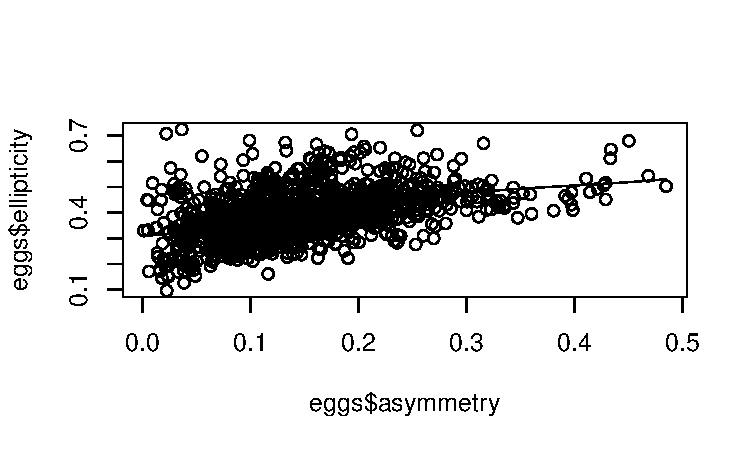
\includegraphics{bookdown-demo_files/figure-latex/unnamed-chunk-83-1.pdf}

\begin{center}\rule{0.5\linewidth}{\linethickness}\end{center}

\section{\texorpdfstring{\protect\hyperlink{section-3}{} The wildlifeR
packge
webiste}{ The wildlifeR packge webiste}}\label{the-wildlifer-packge-webiste}

Some packages have websites that summarize the package contents. If you
visit \url{https://brouwern.github.io/wildlifeR/} you can find out
information on each dataset and function under the ``Reference'' tab,
and see how the datasets and functions are used under the ``Articles''
tab.

\chapter{Loading data from the
internet}\label{loading-data-from-the-internet}

\textbf{Nathan Brouwer, Phd}\\
brouwern at gmail.com\\
\url{https://github.com/brouwern}\\
Twitter: lobrowR

\section{Introduction}\label{introduction-3}

Its possible to download data directly from the internet, including

\begin{itemize}
\tightlist
\item
  Spreadsheets directly posted online as .csv or .txt
\item
  Spreadsheets contained within a GitHub repository, including a package
\item
  Google Sheets
\item
  and many other formats
\end{itemize}

In this short exercise we'll download some data that is stored as a raw
.csv file within the inner workings of the widlifeR package.

\subsection{Learning Goals \& Outcomes}\label{learning-goals-outcomes}

By the end of this lesson students should be able to download basic data
sources from the internet using getURL() from the RCUrl package.

\subsection{Functions \& Arguements}\label{functions-arguements-2}

\begin{itemize}
\tightlist
\item
  RCurl::getURL()
\item
  scatter.smooth
\end{itemize}

\subsection{Packages}\label{packages-3}

\begin{itemize}
\tightlist
\item
  RCurl install.packages()
\end{itemize}

\subsection{Potential hangups}\label{potential-hangups-2}

\begin{itemize}
\tightlist
\item
  Bad internet connection
\item
  Firewall problems
\end{itemize}

\section{\texorpdfstring{\protect\hyperlink{section-3}{} Downloading a
.csv file using
getURL()}{ Downloading a .csv file using getURL()}}\label{downloading-a-.csv-file-using-geturl}

The package RCurl provides functions for accessing online material.
First we need the package

\begin{Shaded}
\begin{Highlighting}[]
\KeywordTok{install.packages}\NormalTok{(}\StringTok{"RCurl"}\NormalTok{, }\DataTypeTok{dependencies =} \OtherTok{TRUE}\NormalTok{) }\CommentTok{# [ ]}
\end{Highlighting}
\end{Shaded}

As always, once we install a package we need to \textbf{really} install
it with library(). (You might see some red text as RCurl loads up some
of its \textbf{dependencies})

\begin{Shaded}
\begin{Highlighting}[]
\KeywordTok{library}\NormalTok{(RCurl) }\CommentTok{# [ ]}
\end{Highlighting}
\end{Shaded}

We then use the getURL() to prep the info we need for downloading that
.csv we want.

The file we want is ``eaglesWV.csv''. It is located at this rather long
URL:\\
\url{https://raw.githubusercontent.com/brouwern/wildlifeR/master/inst/extdata/eaglesWV.csv}

First, we'll use the ``\textless{}-'' assignment operator to store the
shortened URL in an R object. Be sure to put the URL in quotes.

\begin{Shaded}
\begin{Highlighting}[]
\NormalTok{eaglesWV.url <-}\StringTok{ "https://raw.githubusercontent.com/brouwern/wildlifeR/master/inst/extdata/eaglesWV.csv"} \CommentTok{# [ ]}
\end{Highlighting}
\end{Shaded}

Next we'll use the getURL() function to set things up, storing the info
in a new object ``eaglesWV.url\_2'' (note the ``\_2" on the end).

First, get the URL from the URL-containing object we just made.

\begin{Shaded}
\begin{Highlighting}[]
\NormalTok{eaglesWV.url_}\DecValTok{2}\NormalTok{ <-}\StringTok{ }\KeywordTok{getURL}\NormalTok{(eaglesWV.url)}
\end{Highlighting}
\end{Shaded}

Now use read.csv() to actually get it.

\begin{Shaded}
\begin{Highlighting}[]
\NormalTok{eaglesWV_}\DecValTok{2}\NormalTok{ <-}\StringTok{ }\KeywordTok{read.csv}\NormalTok{(}\DataTypeTok{text =}\NormalTok{ eaglesWV.url_}\DecValTok{2}\NormalTok{)}
\end{Highlighting}
\end{Shaded}

We can preview the downloaded dataset using summary() or any other
command we want

\begin{Shaded}
\begin{Highlighting}[]
\KeywordTok{summary}\NormalTok{(eaglesWV_}\DecValTok{2}\NormalTok{)}
\end{Highlighting}
\end{Shaded}

\begin{verbatim}
##       year            WV        
##  Min.   :1980   Min.   : 0.000  
##  1st Qu.:1994   1st Qu.: 4.000  
##  Median :2001   Median : 5.000  
##  Mean   :2001   Mean   : 6.882  
##  3rd Qu.:2008   3rd Qu.:10.000  
##  Max.   :2015   Max.   :19.000  
##                 NA's   :12
\end{verbatim}

\begin{center}\rule{0.5\linewidth}{\linethickness}\end{center}

\section{OPTIONAL: Plotting West Virginia Eagle
Data}\label{optional-plotting-west-virginia-eagle-data}

\textbf{This section is optional}

Thankfully, eagles having been increasing exponentially in West Virginia
since the 1980s.

\begin{Shaded}
\begin{Highlighting}[]
\KeywordTok{scatter.smooth}\NormalTok{(}\DataTypeTok{y =}\NormalTok{ eaglesWV_}\DecValTok{2}\OperatorTok{$}\NormalTok{WV,}\DataTypeTok{x =}\NormalTok{ eaglesWV_}\DecValTok{2}\OperatorTok{$}\NormalTok{year)}
\end{Highlighting}
\end{Shaded}

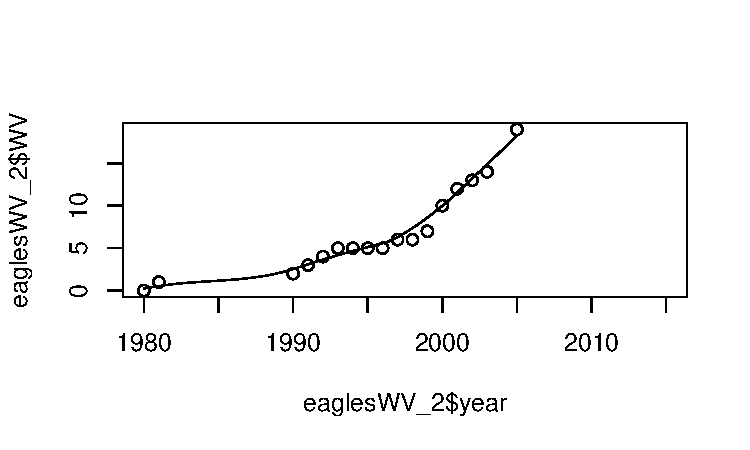
\includegraphics{bookdown-demo_files/figure-latex/unnamed-chunk-90-1.pdf}

\textbf{End optional section}

\begin{center}\rule{0.5\linewidth}{\linethickness}\end{center}

\chapter{Loading data from .csv files into
RStudio}\label{loading-data-from-.csv-files-into-rstudio}

\textbf{Nathan Brouwer, Phd}\\
brouwern at gmail.com\\
\url{https://github.com/brouwern}\\
Twitter: lobrowR

\section{Introduction}\label{introduction-4}

We will be working with data from Table 2 of
\href{https://www.jstor.org/stable/2641255}{Medley and Clements (1998)}.
(This data is featured in the ecological stats book by Quinn and Keough
(2002), though I'm not a fan of how they analyse it.) The paper looks at
how
\href{https://en.wikipedia.org/wiki/Diatom}{diatoms}(photosynthesizing
microorganisms known for their silica shells) are impacted by water
quality in mountain streams.

\subsection{Learning goals}\label{learning-goals-2}

\subsection{Learning objectives}\label{learning-objectives-2}

By the end of this lesson students will be able to

\begin{itemize}
\tightlist
\item
  Download raw data files by hand from the internet
\item
  Load .csv files using the R command read.csv()
\item
  Load .csv files using RStudio's point-and-click interface
\end{itemize}

\subsection{R packageas}\label{r-packageas}

\subsection{R commands}\label{r-commands-1}

\begin{itemize}
\tightlist
\item
  read.csv
\item
  View
\item
  setwd
\item
  getwd
\item
  list.files
\item
  read.csv
\item
  ls
\item
  dim
\item
  names
\item
  summary
\end{itemize}

\subsection{Files}\label{files}

\begin{itemize}
\tightlist
\item
  Medley1998.csv
\end{itemize}

\subsection{Potential Hangups}\label{potential-hangups-3}

\subsection{References}\label{references}

Medley \& Clements. 1998. Responses of diatom communities to heavy
metals in streams: The influence of longitudinal variation.
{[}Ecological Applications 8:631-644.{]}
(\url{https://www.jstor.org/stable/2641255})

Quinn \& Keough. 2002.
\href{http://www.cambridge.org/us/academic/subjects/life-sciences/ecology-and-conservation/experimental-design-and-data-analysis-biologists?format=PB\&isbn=9780521009768\#1HKJ7hG4zeY15ipR.97}{Experimental
design and data analysis for biologists.}. A pdf version of the book is
available online for free..

\section{Preliminary step: download a .csv
file}\label{preliminary-step-download-a-.csv-file}

To load a .csv file into R we first need a .csv file to load. The data
we'll be working with can be downloaded from GitHub. First, go to the
following link (it happens to be an obscure subfolder of the wildlifeR
package)

\url{https://github.com/brouwern/wildlifeR/tree/master/inst/extdata}

Next, locate the file Medley1998.csv

\begin{figure}
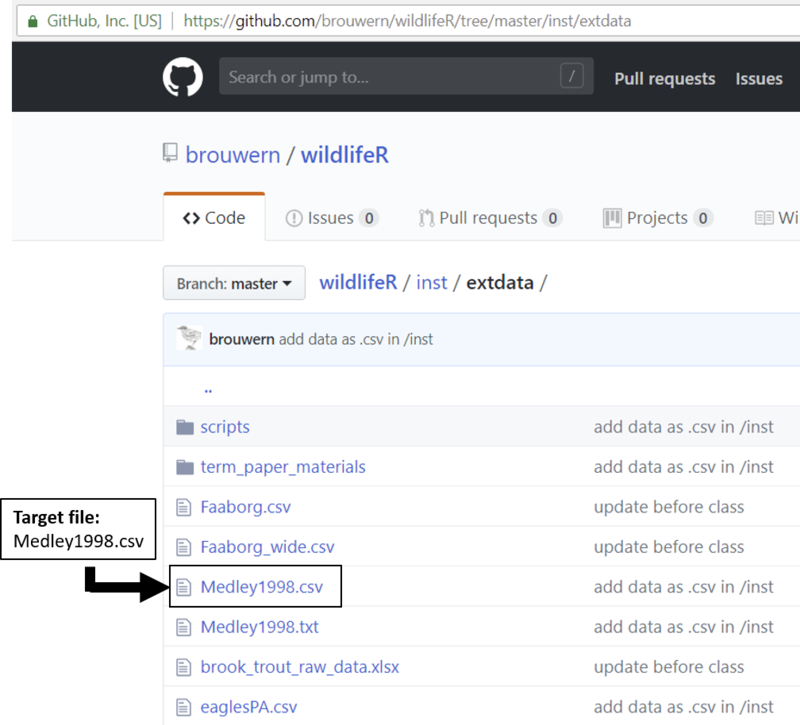
\includegraphics[width=11.11in]{C:/Users/lisanjie/Documents/1_R/git/git-teaching/teaching_2018_2019/2018_fall/biostats_fall_2018/4_biostats_bks_pkg/EDS/EDSbook/./images/Medley1998csv/Medley1998csv-800x1} \caption{A list of files stored on GitHub.}\label{fig:unnamed-chunk-91}
\end{figure}

Click on it; a table will show up.

\begin{figure}
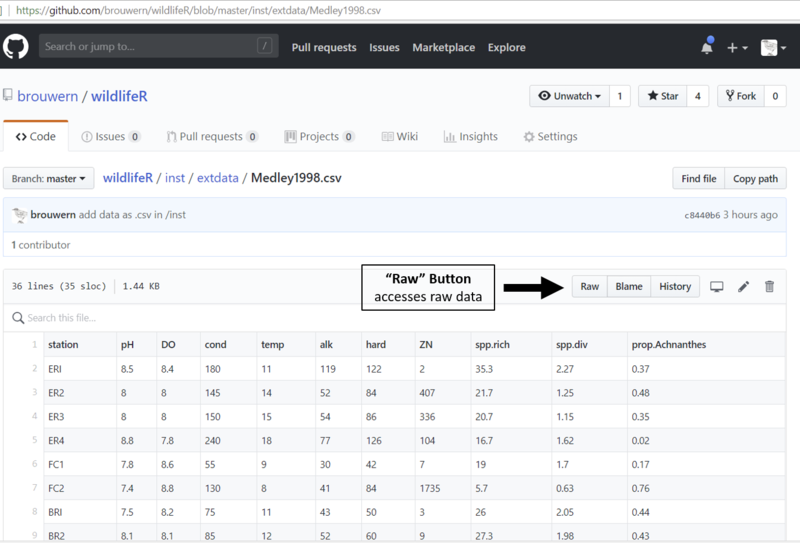
\includegraphics[width=11.11in]{C:/Users/lisanjie/Documents/1_R/git/git-teaching/teaching_2018_2019/2018_fall/biostats_fall_2018/4_biostats_bks_pkg/EDS/EDSbook/images/Medley1998csv/Medley1998csv-800x2} \caption{An HTML .csv datafile store on GitHub.  The raw file can be accessed by clicking on the Raw tab.}\label{fig:unnamed-chunk-92}
\end{figure}

This table is formatted to look nice on a webpage (using some HTML that
GitHub impose on the file). We want the raw file itself. To get it we
need to click on the \textbf{``Raw''} tab.

\begin{figure}
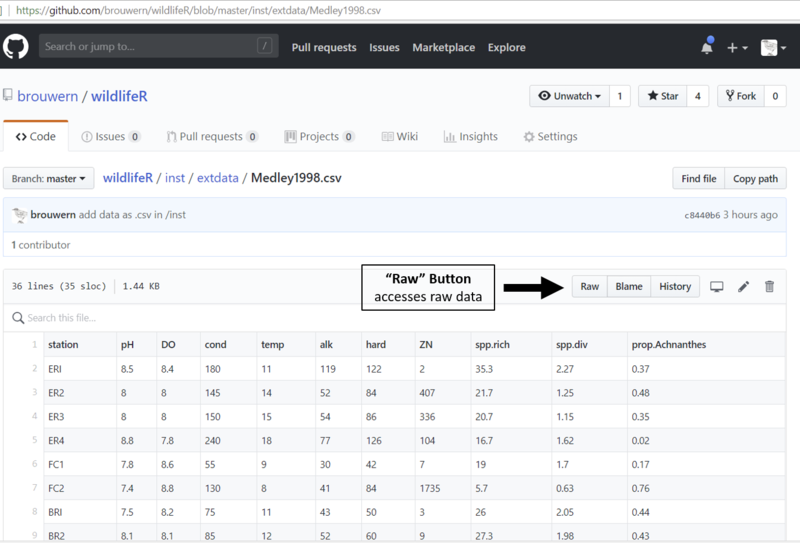
\includegraphics[width=11.11in]{C:/Users/lisanjie/Documents/1_R/git/git-teaching/teaching_2018_2019/2018_fall/biostats_fall_2018/4_biostats_bks_pkg/EDS/EDSbook/images/Medley1998csv/Medley1998csv-800x2} \caption{A raw .csv datafile stored on GitHub.  It can be downloaded By using Crtl+S or right clicking and selecting Save As}\label{fig:unnamed-chunk-93}
\end{figure}

We will then see what looks like a text document against a white
background with no formatting of any kind. We can now download the file
by following these steps.

Either

\begin{itemize}
\tightlist
\item
  Use the shortcut \textbf{Control + S} to ``Save as'' the file
\end{itemize}

Or

\begin{itemize}
\tightlist
\item
  Right click (on Mac:\ldots{})
\item
  ``Save link as'' (or the equivalent)
\end{itemize}

Then save the file to a location you know you can find, such as

\begin{itemize}
\tightlist
\item
  Documents
\item
  Desktop
\item
  Your network profile drive
\end{itemize}

Note that if you try to ``Save as\ldots{}'' anything else but the
white-screen \textbf{raw text file} you will run into problems.

After you download the file, open up Excel or another spreadsheet
program and open up the file to confirm that what you downloaded is just
a set of numbers. I you see long lines of text you might have
accidentally downloaded the HTML-formatted version of the file. Make
sure you are downloading the very plain version of the file from the
totally blank white screen.

\section{\texorpdfstring{Set the ``working directory'' (``WD'') in
RStudio}{Set the working directory (WD) in RStudio}}\label{set-the-working-directory-wd-in-rstudio}

We will now take the data we saved as a .csv file and load it into R.
This can be tricky. First we need to tell R exactly where the file is by
setting the \textbf{working directory}.

Follow these steps:

\begin{itemize}
\tightlist
\item
  Click on ``Session'' on the main menu

  \begin{itemize}
  \tightlist
  \item
    on the menu: ``File, Edit, Code, View, Plots, \textbf{Session},
    \ldots{}''
  \end{itemize}
\item
  Click on ``Set working directory''
\item
  Select ``Choose Directory''
\item
  Select your computer's Documents folder or wherever else you chose to
  save the file.
\item
  Select the directory \& click ``Open''
\item
  Note that the command ``setwd()'' shows up in the console followed by
  the location of the directory you selected
\end{itemize}

You can set your working directory to be anywhere on the computer. It is
essential to make sure that the csv file you want to load into R is in
your working directory.

Depending on the location you chose you might just see
``\textasciitilde{}/'' or some other shorthand.

\section{Check the working directory with
getwd()}\label{check-the-working-directory-with-getwd}

You can confirm where you are at using the command \textbf{getwd()};
this can be handy if you're not sure that you did things correctly or if
R didn't output what you expected.

\begin{Shaded}
\begin{Highlighting}[]
\KeywordTok{getwd}\NormalTok{() }\CommentTok{# [ ]}
\end{Highlighting}
\end{Shaded}

\begin{verbatim}
## [1] "C:/Users/lisanjie/Documents/1_R/git/git-teaching/teaching_2018_2019/2018_fall/biostats_fall_2018/4_biostats_bks_pkg/EDS/EDSbook"
\end{verbatim}

Here, even though when set the working directory R originally just
displayed ``setwd(''\textasciitilde{}/``)'', I can now confirm that I'm
in my documents folder.

\section{Check for the file you downloaded with
list.files()}\label{check-for-the-file-you-downloaded-with-list.files}

You can see what's in your working directory using the command
\textbf{list.files()}. Depending on how many files you have this could
be a very long list. I have 40-ish files and so won't display them.

\begin{Shaded}
\begin{Highlighting}[]
\KeywordTok{list.files}\NormalTok{() }\CommentTok{# [ ]}
\end{Highlighting}
\end{Shaded}

If you have a ton of files being printed out you can narrow things down
by telling R a text pattern to screen for.

\begin{Shaded}
\begin{Highlighting}[]
\KeywordTok{list.files}\NormalTok{(}\DataTypeTok{pattern =} \StringTok{"csv"}\NormalTok{) }\CommentTok{# [ ]}
\end{Highlighting}
\end{Shaded}

\begin{verbatim}
## character(0)
\end{verbatim}

If the file wasn't successful downloaded R will just give you a cryptic
message like this.

\begin{Shaded}
\begin{Highlighting}[]
\KeywordTok{list.files}\NormalTok{(}\DataTypeTok{pattern =} \StringTok{"xxxx"}\NormalTok{)}
\end{Highlighting}
\end{Shaded}

This means the file isn't' there and you need to redo the download to
make sure either i)the file actually downloaded and ii)file is saved
where you want it to be.

What we want to see is this

\begin{verbatim}
## character(0)
\end{verbatim}

\begin{center}\rule{0.5\linewidth}{\linethickness}\end{center}

\section{OPTIONAL Interacting with R via the console or the source
viewer}\label{optional-interacting-with-r-via-the-console-or-the-source-viewer}

\textbf{This section is optional}

You can enter R commands directly into the console, or type them into a
\textbf{script file} in the \textbf{source viewer} and then execute.

If you've just been using the console try this:

\begin{itemize}
\tightlist
\item
  Click on the source viewer pane in RStudio
\item
  Type ``getwd()'' in the source viewer
\item
  Click on the ``Run'' button in the upper Right part of the pane
\item
  The getwd() command is sent over to the console and executed
\end{itemize}

\textbf{End optional section}

\begin{center}\rule{0.5\linewidth}{\linethickness}\end{center}

\section{Loading data into R using
read.csv()}\label{loading-data-into-r-using-read.csv}

Copy and paste the .csv file name from the console into the source
viewer then Execute the command ``read.csv(file =''Medley1998.csv``)''.
You can type it but you must be careful to have NO TYPOS. R is
unforgiving when it comes to typos.

If you've done it correctly you'll see the data table printed out in the
console (I show only some of the output).

\begin{Shaded}
\begin{Highlighting}[]
\KeywordTok{read.csv}\NormalTok{(}\DataTypeTok{file =} \StringTok{"Medley1998.csv"}\NormalTok{)}
\end{Highlighting}
\end{Shaded}

\begin{verbatim}
##   station  pH  DO cond temp alk hard   ZN spp.rich spp.div prop.Achnanthes
## 1     ERI 8.5 8.4  180   11 119  122    2     35.3    2.27            0.37
## 2     ER2 8.0 8.0  145   14  52   84  407     21.7    1.25            0.48
## 3     ER3 8.0 8.0  150   15  54   86  336     20.7    1.15            0.35
## 4     ER4 8.8 7.8  240   18  77  126  104     16.7    1.62            0.02
## 5     FC1 7.8 8.6   55    9  30   42    7     19.0    1.70            0.17
## 6     FC2 7.4 8.8  130    8  41   84 1735      5.7    0.63            0.76
\end{verbatim}

You must have the file name in quotation marks and include the ``.csv''.
\emph{Any} small error will cause things to not work.

Here are examples of mistakes that \emph{won't work} (no matter how much
you cuss at it.)

\begin{Shaded}
\begin{Highlighting}[]
\KeywordTok{read.csv}\NormalTok{(}\DataTypeTok{file =}\NormalTok{ Medley1998.csv)     }\CommentTok{#missing quotes " "}
\KeywordTok{read.csv}\NormalTok{(}\DataTypeTok{file =} \StringTok{"Medley1998.csv"}\NormalTok{)   }\CommentTok{#missing .csv}
\KeywordTok{read.csv}\NormalTok{(file }\StringTok{"Medley1998.csv"}\NormalTok{)     }\CommentTok{#missing =}
\end{Highlighting}
\end{Shaded}

Note that R returns error messages in red, but they aren't necessarily
very helpful in figuring out what the problem actually is. This is an
unfortunate feature of R, and reading error messages is a skill that
must be learned.

\subsection{\texorpdfstring{Load data into an R
``object''}{Load data into an R object}}\label{load-data-into-an-r-object}

Now type this: ``med98 \textless{}- read.csv(file
=''Medley1998.csv``)''. The ``\textless{}-'' is the \textbf{assignment
operator}. What happens when you execute this command?

\begin{Shaded}
\begin{Highlighting}[]
\NormalTok{med98 <-}\StringTok{ }\KeywordTok{read.csv}\NormalTok{(}\DataTypeTok{file =} \StringTok{"Medley1998.csv"}\NormalTok{) [ ]}
\end{Highlighting}
\end{Shaded}

It might actually look like not much has happened. But that's good! It
means the data has successful been loaded into R. You have ``assigned''
the data from your file to the ``object'' named ``med98''

\subsection{\texorpdfstring{The assignment operator
``\textless{}-''}{The assignment operator \textless{}-}}\label{the-assignment-operator--}

``\textless{}-'' is called the ``assignment operator''. It is a special
type of R command.

``\textless{}'' usually shares The comma key. Type ``shift + ,'' To get
it.

If you type just ``med98'' and execute it as a command, what happens?

\begin{Shaded}
\begin{Highlighting}[]
\NormalTok{med98}
\end{Highlighting}
\end{Shaded}

\begin{verbatim}
##   station  pH  DO cond temp alk hard   ZN spp.rich spp.div prop.Achnanthes
## 1     ERI 8.5 8.4  180   11 119  122    2     35.3    2.27            0.37
## 2     ER2 8.0 8.0  145   14  52   84  407     21.7    1.25            0.48
## 3     ER3 8.0 8.0  150   15  54   86  336     20.7    1.15            0.35
## 4     ER4 8.8 7.8  240   18  77  126  104     16.7    1.62            0.02
## 5     FC1 7.8 8.6   55    9  30   42    7     19.0    1.70            0.17
## 6     FC2 7.4 8.8  130    8  41   84 1735      5.7    0.63            0.76
\end{verbatim}

You should see the entire dataset spit out in the console (I've just
shown the top part).

Now execute the list command \textbf{ls()}. You should now see ``med98''
shown in the console.

\begin{Shaded}
\begin{Highlighting}[]
\KeywordTok{ls}\NormalTok{()}
\end{Highlighting}
\end{Shaded}

\begin{verbatim}
##  [1] "crabs"          "eagle.df"       "eagles"         "eaglesWV.url"  
##  [5] "eaglesWV.url_2" "eaglesWV_2"     "iris"           "med98"         
##  [9] "msleep"         "my.abc"         "my.mean"        "x"             
## [13] "year"
\end{verbatim}

This means that the \textbf{object} you assigned your data is now in
your \textbf{``workspace.''} The workspace is what I call the working
memory of R.

We can learn about the med98 data using command like dim(), names() and
summary().

How big is the dataset overall?

\begin{Shaded}
\begin{Highlighting}[]
\KeywordTok{dim}\NormalTok{(med98)}
\end{Highlighting}
\end{Shaded}

\begin{verbatim}
## [1] 34 11
\end{verbatim}

How man columns are there?

\begin{Shaded}
\begin{Highlighting}[]
\KeywordTok{names}\NormalTok{(med98)}
\end{Highlighting}
\end{Shaded}

\begin{verbatim}
##  [1] "station"         "pH"              "DO"             
##  [4] "cond"            "temp"            "alk"            
##  [7] "hard"            "ZN"              "spp.rich"       
## [10] "spp.div"         "prop.Achnanthes"
\end{verbatim}

Are any of the variables categorical?

\begin{Shaded}
\begin{Highlighting}[]
\KeywordTok{summary}\NormalTok{(med98)}
\end{Highlighting}
\end{Shaded}

\begin{verbatim}
##     station         pH              DO             cond       
##  AR2    : 1   Min.   :6.700   Min.   :6.800   Min.   : 40.00  
##  AR3    : 1   1st Qu.:7.425   1st Qu.:7.500   1st Qu.: 76.25  
##  AR5    : 1   Median :7.900   Median :7.600   Median :100.00  
##  AR8    : 1   Mean   :7.841   Mean   :7.794   Mean   :116.76  
##  ARI    : 1   3rd Qu.:8.200   3rd Qu.:8.175   3rd Qu.:150.00  
##  BR2    : 1   Max.   :8.800   Max.   :8.800   Max.   :240.00  
##  (Other):28                                                   
##       temp            alk              hard              ZN        
##  Min.   : 8.00   Min.   : 10.00   Min.   : 10.00   Min.   :   2.0  
##  1st Qu.:11.00   1st Qu.: 28.50   1st Qu.: 45.00   1st Qu.:  24.0  
##  Median :12.50   Median : 46.50   Median : 62.00   Median :  54.0  
##  Mean   :13.06   Mean   : 46.38   Mean   : 66.76   Mean   : 177.3  
##  3rd Qu.:15.00   3rd Qu.: 64.00   3rd Qu.: 90.50   3rd Qu.: 213.2  
##  Max.   :21.00   Max.   :119.00   Max.   :126.00   Max.   :1735.0  
##                                                                    
##     spp.rich        spp.div      prop.Achnanthes 
##  Min.   : 5.70   Min.   :0.630   Min.   :0.0200  
##  1st Qu.:18.77   1st Qu.:1.377   1st Qu.:0.2125  
##  Median :22.85   Median :1.855   Median :0.3900  
##  Mean   :22.42   Mean   :1.694   Mean   :0.3756  
##  3rd Qu.:26.82   3rd Qu.:2.058   3rd Qu.:0.4950  
##  Max.   :42.00   Max.   :2.830   Max.   :0.7600  
## 
\end{verbatim}

\begin{center}\rule{0.5\linewidth}{\linethickness}\end{center}

\section{Optional: Plot the Mendley 1998
data}\label{optional-plot-the-mendley-1998-data}

\textbf{The following section is optional}

As we'll discuss in depth in a later section on plotting , one reason
why the \textbf{ggplot} and \textbf{ggpubr} packages are so powerful is
because they can easily plot things in good color schemes. We can make a
basic scatter plot like this to show the positive correlation between
Diatom species richness (the raw number of species identified in a given
sample) on the x axis and species diversity on the y axis.

First, load the ggpubr package using the library() command. Note that
you might get some output in red text telling you about the packages; it
looks scary but its not.

\begin{Shaded}
\begin{Highlighting}[]
\KeywordTok{library}\NormalTok{(ggpubr)}
\end{Highlighting}
\end{Shaded}

Now plot the scatter plot. Note that the syntax for ggpubr requires that
variables be contained within quotes.

\begin{Shaded}
\begin{Highlighting}[]
\KeywordTok{ggscatter}\NormalTok{(}\DataTypeTok{data =}\NormalTok{ med98, }\DataTypeTok{y =} \StringTok{"spp.div"}\NormalTok{,}\DataTypeTok{x =} \StringTok{"spp.rich"}\NormalTok{)}
\end{Highlighting}
\end{Shaded}

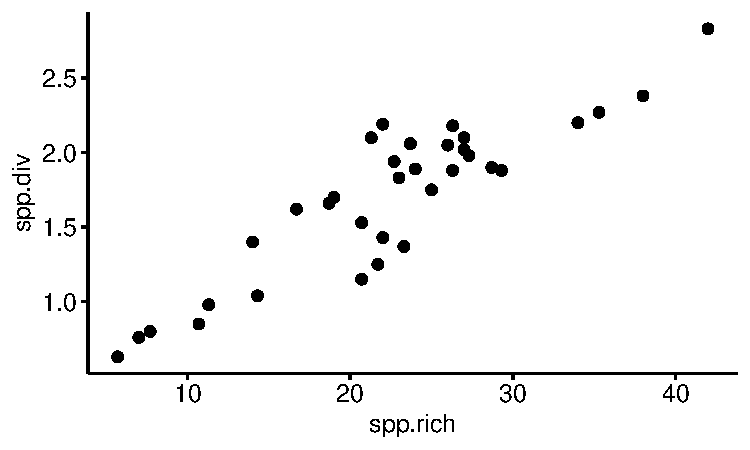
\includegraphics{bookdown-demo_files/figure-latex/unnamed-chunk-110-1.pdf}

We can color-code the points by their pH

\begin{Shaded}
\begin{Highlighting}[]
\KeywordTok{ggscatter}\NormalTok{(}\DataTypeTok{data =}\NormalTok{ med98, }\DataTypeTok{y =} \StringTok{"spp.div"}\NormalTok{,}\DataTypeTok{x =} \StringTok{"spp.rich"}\NormalTok{, }\DataTypeTok{color =} \StringTok{"pH"}\NormalTok{)}
\end{Highlighting}
\end{Shaded}

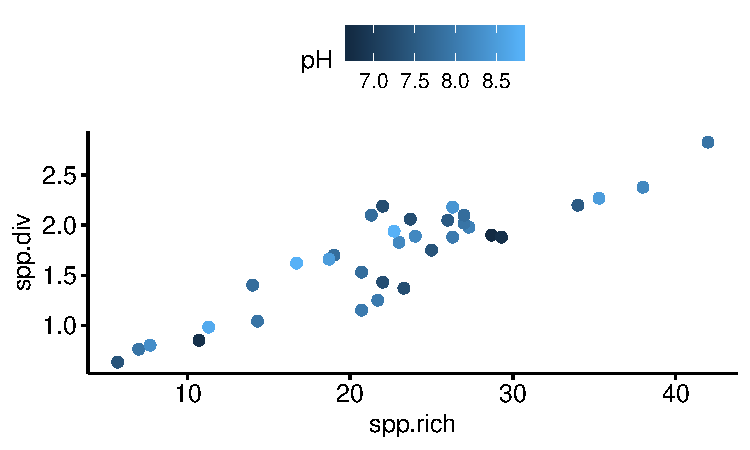
\includegraphics{bookdown-demo_files/figure-latex/unnamed-chunk-111-1.pdf}

\textbf{End optional section}

\begin{center}\rule{0.5\linewidth}{\linethickness}\end{center}

\section{\texorpdfstring{Loading .csv files using RStudio
\protect\hyperlink{section-3}{}}{Loading .csv files using RStudio }}\label{loading-.csv-files-using-rstudio}

Frequently in code I will have things written up to load data using the
\textbf{read.csv()} command. However, there is a point-and-click way of
loading spreadsheet data into RStudio too.

There's on pane in RStudio that doesn't get used much by basic R users,
the ``Environment, History, Connections, Build, Git'' pane (I think it
might not have ``Git'' on it if you don't have certain packages loaded).

\begin{figure}
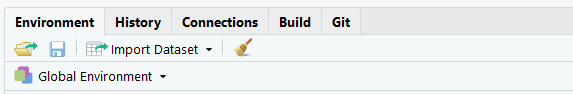
\includegraphics[width=7.96in]{C:/Users/lisanjie/Documents/1_R/git/git-teaching/teaching_2018_2019/2018_fall/biostats_fall_2018/4_biostats_bks_pkg/EDS/EDSbook/images/Environment_tab_import_dataset_1} \caption{A list of files stored on GitHub.}\label{fig:unnamed-chunk-112}
\end{figure}

If you click on the spreadsheet-looking icon ``Import Dataset'' and
select ``From text (base)'' you can navigate to where your .csv file is
located and select it. A preview window will then pop up which will show
you the raw (which should look like what you originally down loaded) and
a preview of how RStudio will format the data. (If the preview doesn't
look right you can change some of the option in the drop down menus to
see if things line up.)

\begin{figure}
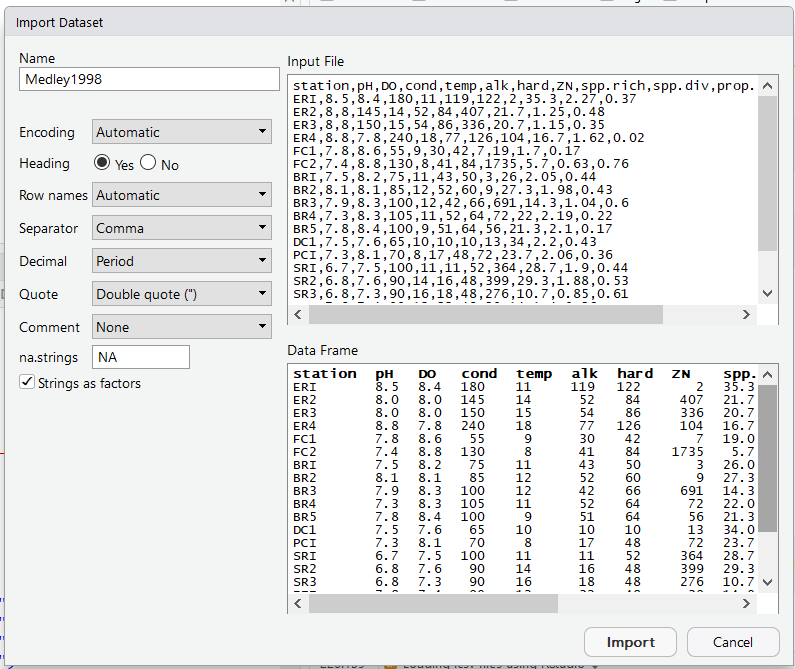
\includegraphics[width=11.04in]{C:/Users/lisanjie/Documents/1_R/git/git-teaching/teaching_2018_2019/2018_fall/biostats_fall_2018/4_biostats_bks_pkg/EDS/EDSbook/images/Environment_tab_import_dataset_2} \caption{A list of files stored on GitHub.}\label{fig:unnamed-chunk-113}
\end{figure}

When you click ``Import'' RStudio will execute some code in the console
(eg ``Medley1998 \textless{}-
read.csv(''\textasciitilde{}/Medley1998.csv``)'') to load the data and
then call the command \textbf{View()} to generate preview of the data in
a new tab in the script view. (Note that this View panel only lets you
look at the data; you can't edit it.)

\section{Challenge}\label{challenge-2}

.csv files are the most common format for sharing data in R. ``csv''
stands for ``comma seperate volume'', and you will note that each value
on a line is seperated by a comma (some things with computers do make
sense on the first try!).

Sometimes you will encounter .txt files which separate data other ways,
such as spaces, tabs, or by lining up everything explicitly in rows. On
the wildlifeR GitHub directory we used before
(\url{https://github.com/brouwern/wildlifeR/tree/master/inst/extdata})
these is a file ``Medley1998.txt''. Download this file and load it using
RStudio's Import Dataset function. See if RStudio recognizes that its
not .csv.

\chapter{Loading Excel spreadsheets into
RStudio}\label{loading-excel-spreadsheets-into-rstudio}

\textbf{Nathan Brouwer, Phd}\\
brouwern at gmail.com\\
\url{https://github.com/brouwern}\\
Twitter: lobrowR

\textbf{THIS CHAPTER HAS NOT BEEN WRITTEN}

re-save as .csv and load

load directly

In this walk through we first re-save this data in an R-compatible
format, a ``csv'' file, called ``Lab1\_data\_PA\_eagles.csv''.

\subsection{Prepping data in Excel}\label{prepping-data-in-excel}

\subsubsection{Save data to your R working directory
(WD)}\label{save-data-to-your-r-working-directory-wd}

Find the file
\url{https://github.com/brouwern/wildlifeR/tree/master/inst/extdata}

Save the file ``Lab1\_data\_PA\_eagles.xlsx'' to your computers desktop.
Today we will be using this as the ``working directory''

\subsubsection{\texorpdfstring{Re-Save The Excel file as a ``csv''
file}{Re-Save The Excel file as a csv file}}\label{re-save-the-excel-file-as-a-csv-file}

In Excel, follow these steps

\begin{itemize}
\tightlist
\item
  ``File''
\item
  ``Save As''
\item
  ``Browse''
\item
  Select the working directory (your desktop)
\item
  Select ``Save as type''
\item
  Select ``CSV (Comma delimited)''
\item
  Click ``Save''
\end{itemize}

The data is now in a format that can be loaded into R.

\section{Preparing a file for loading into
R}\label{preparing-a-file-for-loading-into-r}

Things work best when your Excel file is ``clean'' \& only has exactly
what you want in it. Any extra, accidental typing can cause problems or
make things confusing. A good practice is to always highlight cells to
the right of and below your data, right click \& select ``Delete''. This
will remove any accidental typing that occurred. Do this to the cells
below your data also.

\section{Reload data}\label{reload-data}

Reload data; be sure to include the ``csv'' at the end. Use this code
``eaglesPA \textless{}- read.csv(file =''eaglesPA.xlsx``)''. NOTE: I
changed the name of the file to include ``\_w\_2\_states" so that I
wouldn't overwrite the original file. Don't use this code unless you
changed the file name to the exact same thing

\begin{Shaded}
\begin{Highlighting}[]
\CommentTok{#Use this code, w/o the "#" in front of it}
\CommentTok{# eaglesPA <- read.csv(file = "eaglesPA.xlsx")}

\CommentTok{#NOTE: I changed the name of the file to include "_w_2_states" so that I wouldn't overwrite the origina file.  Don't use this code unless you changed the file name to the exact smame thing}
\CommentTok{#eaglesPA <- read.csv(file = "./data/Lab1_data_PA_eaglesPA_w_2_states.csv")}
\end{Highlighting}
\end{Shaded}

Type ls() to see what is now in your workspace

\begin{Shaded}
\begin{Highlighting}[]
\KeywordTok{ls}\NormalTok{()}
\end{Highlighting}
\end{Shaded}

\begin{verbatim}
##  [1] "crabs"          "eagle.df"       "eagles"         "eaglesWV.url"  
##  [5] "eaglesWV.url_2" "eaglesWV_2"     "iris"           "med98"         
##  [9] "msleep"         "my.abc"         "my.mean"        "x"             
## [13] "year"
\end{verbatim}

Look at the re-loaded eaglesPA data object

\begin{Shaded}
\begin{Highlighting}[]
\KeywordTok{summary}\NormalTok{(eaglesPA)}
\KeywordTok{dim}\NormalTok{(eaglesPA)}
\KeywordTok{head}\NormalTok{(eaglesPA)}
\KeywordTok{tail}\NormalTok{(eaglesPA)}
\end{Highlighting}
\end{Shaded}

\part{Plotting data in R with ggplot2 \&
friends}\label{part-plotting-data-in-r-with-ggplot2-friends}

\subsection*{}\label{section-2}
\addcontentsline{toc}{subsection}{}

In this section we'll focus on basic plotting skills. The first chapter
in this section is a review of the skills needed to get some data into R
from a package. Subsequent chapters will develop plotting skills with a
focus on using ggplot2.

We'll briefly go over all aspects of \textbf{ggplot2} and its varients.
This will orient you to the different things you are likely to see other
R users use. For most of this book, however, we'll focus on a package
which creates a ``wrapper'' for ggplot2 called
\href{http://www.sthda.com/english/rpkgs/ggpubr/}{ggpubr} which speeds
up the process for beginners of making publication-ready graphs. Even if
you are a ggplot2 pro you should know about ggpubr for making quick
graphs, and for teaching others about ggplot2.

\chapter{Review: Loading \& Examining Data in
R}\label{review-loading-examining-data-in-r}

\textbf{Nathan Brouwer, Phd}\\
brouwern at gmail.com\\
\url{https://github.com/brouwern}\\
Twitter: lobrowR

\section{Introduction}\label{introduction-5}

This exercise reviews the basics of loading data from a package into R.
These basic skills are needed for the further tasks of plotting that
will be built upon in this section. If you are familiar with R you can
probably skim this or skip it altogether. If you are brand new then this
is an excellent review of the material covered so far in this book.

\subsection{Learning Goals \& Outcomes}\label{learning-goals-outcomes-1}

To review the basics of loading packages and data.

\subsection{Functions \& Arguements}\label{functions-arguements-3}

\begin{itemize}
\tightlist
\item
  data
\item
  library
\item
  ls
\item
  dim
\item
  names
\item
  head
\item
  tail
\item
  is
\item
  summary
\item
  install.packages
\end{itemize}

\subsection{Packages}\label{packages-4}

\begin{itemize}
\tightlist
\item
  MASS
\item
  cowplot
\end{itemize}

\subsection{Outline}\label{outline}

\begin{itemize}
\tightlist
\item
  Intro
\item
  Fisher's Iris data
\item
  Loading data: iris
\item
  The easy way: from base R w/ data(iris)
\item
  Loading packages in base R: MASS
\item
  command: library(MASS)
\item
  Loading packages from CRAN: cowplot
\end{itemize}

\section{Example data for plotting: Fisher's
Irises}\label{example-data-for-plotting-fishers-irises}

\begin{itemize}
\tightlist
\item
  Dataset made popular by R.A. Fisher
\item
  Frequently used to explain/test stats procedures
\item
  See ?iris for more details
\item
  See also \url{https://en.wikipedia.org/wiki/Iris_flower_data_set} for
  more info.
\end{itemize}

\section{\texorpdfstring{Loading data into R the easy way: pre-made data
in an R
``Package''}{Loading data into R the easy way: pre-made data in an R Package}}\label{loading-data-into-r-the-easy-way-pre-made-data-in-an-r-package}

\begin{itemize}
\tightlist
\item
  Getting data into R (or SAS, or ArcGIS\ldots{}) can be a pain!
\item
  R comes with many datasets that are pre-loaded into it
\item
  There are also many stat. techniques that can easily be added to R
\item
  These are contained in ``packages''
\end{itemize}

\subsection{\texorpdfstring{Load data that is already in the ``base''
distribution of
R}{Load data that is already in the base distribution of R}}\label{load-data-that-is-already-in-the-base-distribution-of-r}

Fisher's iris data comes automatically with R. You can load it into R's
memory using the command ``data()''

\begin{Shaded}
\begin{Highlighting}[]
\KeywordTok{data}\NormalTok{(iris) }\CommentTok{#Load the iris data}
\end{Highlighting}
\end{Shaded}

\subsection{Look at the iris data}\label{look-at-the-iris-data}

We'll look at the iris data using some commands like ls(), dim(), and
names().

You can check that it was loaded using the \textbf{ls()} command
(``list'').

\begin{Shaded}
\begin{Highlighting}[]
\KeywordTok{ls}\NormalTok{()}
\end{Highlighting}
\end{Shaded}

You can get info about the nature of the dataframe using commands like
\textbf{dim()}

\begin{Shaded}
\begin{Highlighting}[]
\KeywordTok{dim}\NormalTok{(iris)}
\end{Highlighting}
\end{Shaded}

This tells us that the iris data is essentially a spreadsheet that has
150 rows and 5 columns.

We can get the column names with names()

\begin{Shaded}
\begin{Highlighting}[]
\KeywordTok{names}\NormalTok{(iris)}
\end{Highlighting}
\end{Shaded}

\begin{itemize}
\tightlist
\item
  Note that the first letter of each word is capitalized.\\
\item
  What are the implications of this?
\end{itemize}

The top of the data and the bottom of the data can be checked with
head() and tail() commands

\begin{Shaded}
\begin{Highlighting}[]
\KeywordTok{head}\NormalTok{(iris) }\CommentTok{#top of dataframe}

\KeywordTok{tail}\NormalTok{(iris) }\CommentTok{#bottom of dataframe}
\end{Highlighting}
\end{Shaded}

Another common R command is \textbf{is()}, which tells you what
something is in R land.

\begin{Shaded}
\begin{Highlighting}[]
\KeywordTok{is}\NormalTok{(iris)}
\end{Highlighting}
\end{Shaded}

\begin{itemize}
\tightlist
\item
  R might spew a lot of things out at you when you use \textbf{is()}
\item
  usually the 1st item is most important.\\
\item
  Here, it tells us that the ``object'' called ``iris'' in your
  workspace is 1st and foremost a ``data.frame''
\item
  A dataframe is essentially a spreadsheet of data loaded into R.
\end{itemize}

You can get basic info about the data themselves using commands like
\textbf{summary()}.

\begin{Shaded}
\begin{Highlighting}[]
\KeywordTok{summary}\NormalTok{(iris)}
\end{Highlighting}
\end{Shaded}

\begin{itemize}
\tightlist
\item
  Which variables are numeric?
\item
  Which variables are categories/groups (aka ``factors'')?
\end{itemize}

If you wanted info on just 1 column, you would tell R to isolate that
column like this, using a dollar sign (\$).

\begin{Shaded}
\begin{Highlighting}[]
\KeywordTok{summary}\NormalTok{(iris}\OperatorTok{$}\NormalTok{Sepal.Width)}
\end{Highlighting}
\end{Shaded}

That is, that name of the dataframe, a dollar sign (\$), and the name of
the column.

What happens when you don't capitalize something? Try these intentional
mistakes (but remove the ``\#'' from in front of each one):

\begin{Shaded}
\begin{Highlighting}[]
\CommentTok{#all lower case}
\KeywordTok{summary}\NormalTok{(iris}\OperatorTok{$}\NormalTok{sepal.width) }\CommentTok{# this won't work}

\CommentTok{#just "s" in "sepal" lower case}
\KeywordTok{summary}\NormalTok{(iris}\OperatorTok{$}\NormalTok{sepal.Width)  }\CommentTok{#this won't work either}

\CommentTok{#or what if you capitalize "i" in "Iris"?}
\KeywordTok{summary}\NormalTok{(Iris}\OperatorTok{$}\NormalTok{Sepal.Width) }\CommentTok{#won't work either}
\end{Highlighting}
\end{Shaded}

The first two error messages are not very informative; the 3rd one
(``Error in summary(Iris\$Sepal.Width) : object `Iris' not found'') does
make a little sense.

\section{Load data that is in another R
package}\label{load-data-that-is-in-another-r-package}

\subsection{Packages that come with R}\label{packages-that-come-with-r}

\begin{itemize}
\tightlist
\item
  Many scientists develop software for R, and they often include
  datasets to demonstrate how the software works.\\
\item
  Some of this software, called a ``package'' comes with R already and
  just needs to be loaded.\\
\item
  This is done with the \textbf{library()} command.
\item
  The \textbf{MASS} package comes with R when you download it and has
  many useful functions and interesting datasets.
\end{itemize}

\begin{Shaded}
\begin{Highlighting}[]
\KeywordTok{library}\NormalTok{(MASS) }\CommentTok{#Load the MASS package}
\end{Highlighting}
\end{Shaded}

MASS contains a dataset called called ``mammals''

\begin{Shaded}
\begin{Highlighting}[]
\KeywordTok{data}\NormalTok{(mammals)}
\end{Highlighting}
\end{Shaded}

You can confirm that the mammals data is in your workspace using
\textbf{ls()}

\begin{Shaded}
\begin{Highlighting}[]
\KeywordTok{ls}\NormalTok{()}
\end{Highlighting}
\end{Shaded}

You should now have both the ``iris''" and the ``mammals''" data in your
R ``workspace.''"

What is in the mammals dataset? Datasets actually usually have useful
help files. Access help using the \textbf{?} function.

The help screen will pop up either within RStudio, or possibly in your
web browser. It tells us that mammals is

\begin{quote}
``A data frame with average brain and body weights for 62 species of
land mammals.''
\end{quote}

Since this is someone else's data, the authors of the MASS package need
to provide proper citation. At the bottom we can see that these data
come from the paper:

\begin{quote}
Allison, T. and Cicchetti, D. V. (1976) Sleep in mammals: ecological and
constitutional correlates. Science 194: 732-734.
\end{quote}

We can learn about the mammals data using the usual commands

\begin{Shaded}
\begin{Highlighting}[]
\KeywordTok{dim}\NormalTok{(mammals)}
\KeywordTok{names}\NormalTok{(mammals)}
\KeywordTok{head}\NormalTok{(mammals)}
\KeywordTok{tail}\NormalTok{(mammals)}
\KeywordTok{summary}\NormalTok{(mammals)}
\end{Highlighting}
\end{Shaded}

\section{Load Data From A package On
CRAN}\label{load-data-from-a-package-on-cran}

Most packages don't come with R when you download it but are stored in a
central site called CRAN. We'll load data from the \textbf{cowplot}
package.

\subsection{Loading packages using
R-Studio}\label{loading-packages-using-r-studio}

RStudio makes it easy to find and load packages. Follow these
instructions.

\begin{itemize}
\tightlist
\item
  In the panel of RStudio that has the tabs ``Plots'',
  ``Packages'',``Help'', ``Viewer'' click on ``Packages''"
\item
  On the next line it says ``Install'' and ``Update''. Click on
  ``Install''
\item
  A window will pop up. In the white field in the middle of the window
  under ``Packages'' type the name of the package you want.
\item
  RStudio will automatically bring up potential packages as you type.
\item
  Finish typing ``cowplot'' or click on the name.
\item
  Click on the ``Install'' button.
\item
  In the source viewer some misc. test should show up. Most of the time
  this works. If it doesn't, talk to the professor!
\end{itemize}

If an R packages doesn't load properly, it could be for several reasons.

\begin{enumerate}
\def\labelenumi{\arabic{enumi}.}
\tightlist
\item
  Your internet connection might be having problems.\\
\item
  The website where the package is stored might be down for
  maintenance.\\
\item
  The version of are you are using is probably newer than the version of
  R used to make the package. This is a real pain - ask for help from an
  expert R user if think you have this problem.
\end{enumerate}

\section{Loading packages directly using
code}\label{loading-packages-directly-using-code}

You can also use the \textbf{install.packages()} command to try to load
the package.

\begin{Shaded}
\begin{Highlighting}[]
\KeywordTok{install.packages}\NormalTok{(}\StringTok{"cowplot"}\NormalTok{)}
\end{Highlighting}
\end{Shaded}

\section{Troubleshooting Package
Downloads}\label{troubleshooting-package-downloads}

\subsection{What if you tell R to install a package you already have
downloaded?}\label{what-if-you-tell-r-to-install-a-package-you-already-have-downloaded}

If you already have the package downloaded to your computer then a
window will pop up asking you if you want to restart your computer.
Normally this isn't necessary; just click ``no''. You might see a
``warning'' message pop up in the console such as ``Warning in
install.packages: package `cowplot' is in use and will not be
installed''. This isn't a problem for basic R work. If you are doing
serious work (e.g.~for a publication) you should restart R.

\subsection{What if I can't get a package I need
loaded?}\label{what-if-i-cant-get-a-package-i-need-loaded}

\begin{itemize}
\tightlist
\item
  Talk to someone who is good w/R (eg, your professor)
\item
  Google something like ``how to install R package'' for general info
\item
  Google something like ``problem loading R package''
\item
  Copy and paste any error message you might be getting into Google and
  see if anyone has written about this problem
\end{itemize}

See above for reasons why a package might not load properly the 1st time
you try.

\subsection{Finding R help with
Google}\label{finding-r-help-with-google}

There's lots of info about R on the web, and if you have a problem, then
someone else has probably had it before and perhaps written something
about it.

The website \textbf{stackoverflow.com} has lots of info about R.
However, many people who use it are hard-core programmers, who can come
across as jerks sometimes when they answer questions if you don't follow
the rules and protocols of stackoverflow.

\chapter{Plotting Continous Data in R With
ggplot2}\label{plotting-continous-data-in-r-with-ggplot2}

\textbf{Nathan Brouwer, Phd}\\
brouwern at gmail.com\\
\url{https://github.com/brouwern}\\
Twitter: lobrowR

\section{Introduction}\label{introduction-6}

\begin{itemize}
\tightlist
\item
  We're going to plot some data using the qplot() command
\item
  We'll need to have 2 packages loaded
\item
  ggplot2, which has the function qplot()
\item
  cowplot, which provides some nice defaults
\item
  We'll use the iris dataset that comes with R
\end{itemize}

\subsection{Learning goals \&
objectives}\label{learning-goals-objectives}

Introduce the qplot command from the ggplot2 package

\subsection{Functions \& Arguements}\label{functions-arguements-4}

\subsection{Packages}\label{packages-5}

\begin{itemize}
\tightlist
\item
  ggplot2
\item
  cowplot
\end{itemize}

\subsection{Outline}\label{outline-1}

\section{Introduction to ggplot using
qplot}\label{introduction-to-ggplot-using-qplot}

Load the iris data

\begin{Shaded}
\begin{Highlighting}[]
\KeywordTok{data}\NormalTok{(iris)}
\end{Highlighting}
\end{Shaded}

Load the ggplot2 and cowplot packages

\section{A basic plot in ggplot using
qplot()}\label{a-basic-plot-in-ggplot-using-qplot}

Unless you tell it otherwise, qplot plots dots.

\begin{Shaded}
\begin{Highlighting}[]
\KeywordTok{qplot}\NormalTok{(}\DataTypeTok{y =}\NormalTok{ Sepal.Length,}
      \DataTypeTok{x =}\NormalTok{ Species,    }
        \DataTypeTok{data =}\NormalTok{ iris) }
\end{Highlighting}
\end{Shaded}

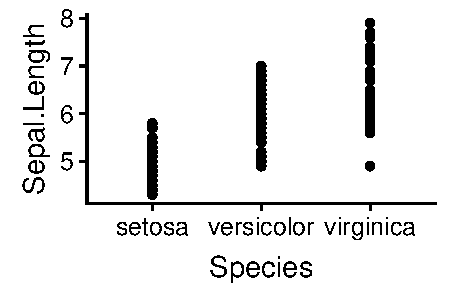
\includegraphics{bookdown-demo_files/figure-latex/unnamed-chunk-133-1.pdf}

\chapter{Box plot with labels}\label{box-plot-with-labels}

\begin{itemize}
\tightlist
\item
  R will usually generate labels for the x and y axes based on the
  command. * These can be changed by adding another command after the
  qplot() command
\item
  Add The command \textbf{+ xlab(``\ldots{}'')} sets the labels for the
  x-axis, \textbf{+ ylab(``\ldots{}'')} for the y axis.
\item
  Text for the labels goes in quotes (ie, ``Iris species'').
\item
  The use of the ``+'' is different than for most other R packages
\item
  Forgetting the quotes will cause the code to fail.\\
\item
  Note that units (mm) are included for the y axis.
\end{itemize}

\begin{Shaded}
\begin{Highlighting}[]
\KeywordTok{qplot}\NormalTok{(}\DataTypeTok{y =}\NormalTok{ Sepal.Length,}
      \DataTypeTok{x =}\NormalTok{ Species,    }
        \DataTypeTok{data =}\NormalTok{ iris) }\OperatorTok{+}\StringTok{         }\CommentTok{# note the "+"}
\StringTok{  }\KeywordTok{xlab}\NormalTok{(}\StringTok{"Iris Species"}\NormalTok{) }\OperatorTok{+}\StringTok{       }\CommentTok{# label for x axis}
\StringTok{  }\KeywordTok{ylab}\NormalTok{ (}\StringTok{"Sepal Length (mm)"}\NormalTok{ )  }\CommentTok{# label for y axis}
\end{Highlighting}
\end{Shaded}

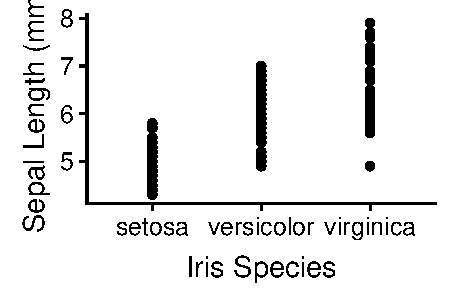
\includegraphics{bookdown-demo_files/figure-latex/unnamed-chunk-134-1.pdf}

\section{Changing colors in R plots}\label{changing-colors-in-r-plots}

\subsection{Changing colors in R plots part
1}\label{changing-colors-in-r-plots-part-1}

\begin{itemize}
\tightlist
\item
  If we wanted we could change the color of the dots using the argument
  \textbf{``col =''}. This code can be used to change the color of most
  types of plots in R.\\
\item
  This doesn't increase the information content of the figure but maybe
  makes it nicer to look at.
\end{itemize}

\begin{Shaded}
\begin{Highlighting}[]
\KeywordTok{qplot}\NormalTok{(}\DataTypeTok{y =}\NormalTok{ Sepal.Length,}
      \DataTypeTok{x =}\NormalTok{ Species,    }
        \DataTypeTok{data =}\NormalTok{ iris,}
      \DataTypeTok{color =} \StringTok{"red"}\NormalTok{) }\OperatorTok{+}
\StringTok{  }\KeywordTok{xlab}\NormalTok{(}\StringTok{"Iris Species"}\NormalTok{) }\OperatorTok{+}\StringTok{  }
\StringTok{  }\KeywordTok{ylab}\NormalTok{ (}\StringTok{"Sepal Length (mm)"}\NormalTok{ )}
\end{Highlighting}
\end{Shaded}

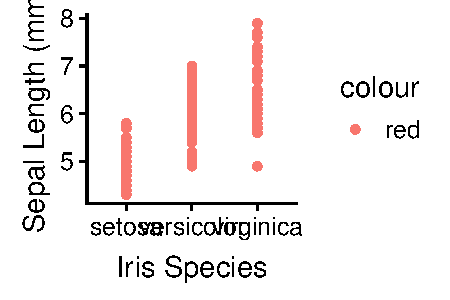
\includegraphics{bookdown-demo_files/figure-latex/unnamed-chunk-135-1.pdf}

\subsection{Changing colors in R plots part
2}\label{changing-colors-in-r-plots-part-2}

\begin{Shaded}
\begin{Highlighting}[]
\CommentTok{#dopt w/color changes}
\KeywordTok{qplot}\NormalTok{(}\DataTypeTok{y =}\NormalTok{ Sepal.Length,}
      \DataTypeTok{x =}\NormalTok{ Species,    }
        \DataTypeTok{data =}\NormalTok{ iris,}
      \DataTypeTok{color =}\NormalTok{ Species) }\OperatorTok{+}
\StringTok{  }\KeywordTok{xlab}\NormalTok{(}\StringTok{"Iris Species"}\NormalTok{) }\OperatorTok{+}\StringTok{  }
\StringTok{  }\KeywordTok{ylab}\NormalTok{ (}\StringTok{"Sepal Length (mm)"}\NormalTok{)}
\end{Highlighting}
\end{Shaded}

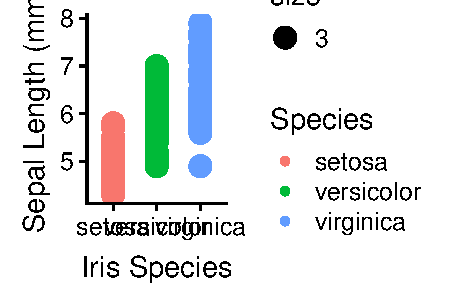
\includegraphics{bookdown-demo_files/figure-latex/unnamed-chunk-136-1.pdf}

\section{Tweaking plots: changing the point
size}\label{tweaking-plots-changing-the-point-size}

Run the code below, Can you see what changed?

\begin{Shaded}
\begin{Highlighting}[]
\CommentTok{#dopt w/color changes}
\KeywordTok{qplot}\NormalTok{(}\DataTypeTok{y =}\NormalTok{ Sepal.Length,}
      \DataTypeTok{x =}\NormalTok{ Species,    }
        \DataTypeTok{data =}\NormalTok{ iris,}
      \DataTypeTok{color =}\NormalTok{ Species,}
      \DataTypeTok{size =} \DecValTok{3}\NormalTok{) }\OperatorTok{+}
\StringTok{  }\KeywordTok{xlab}\NormalTok{(}\StringTok{"Iris Species"}\NormalTok{) }\OperatorTok{+}\StringTok{  }
\StringTok{  }\KeywordTok{ylab}\NormalTok{ (}\StringTok{"Sepal Length (mm)"}\NormalTok{)}
\end{Highlighting}
\end{Shaded}

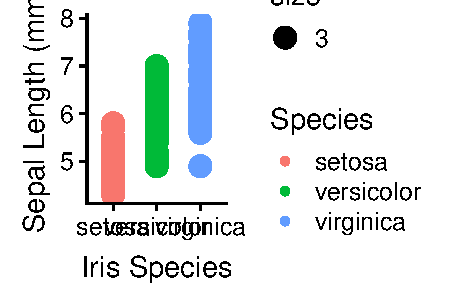
\includegraphics{bookdown-demo_files/figure-latex/unnamed-chunk-137-1.pdf}

\section{Boxplot with qplot}\label{boxplot-with-qplot}

\subsection{Basic boxplot with qplot}\label{basic-boxplot-with-qplot}

\begin{itemize}
\tightlist
\item
  note use of arguement \textbf{``geom = \ldots{}''}
\end{itemize}

\begin{Shaded}
\begin{Highlighting}[]
\KeywordTok{qplot}\NormalTok{(}\DataTypeTok{y =}\NormalTok{ Sepal.Length,}
      \DataTypeTok{x =}\NormalTok{ Species,    }
        \DataTypeTok{data =}\NormalTok{ iris,}
      \DataTypeTok{geom =} \StringTok{"boxplot"}\NormalTok{) }
\end{Highlighting}
\end{Shaded}

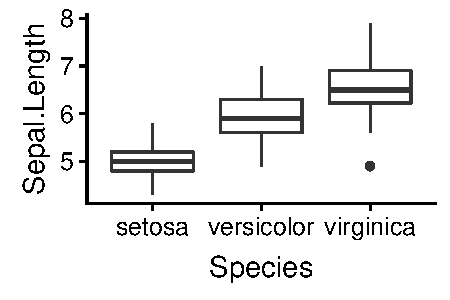
\includegraphics{bookdown-demo_files/figure-latex/unnamed-chunk-138-1.pdf}

\section{Basic boxplot with colors}\label{basic-boxplot-with-colors}

\begin{itemize}
\tightlist
\item
  same as before, using ``color =''
\end{itemize}

\begin{Shaded}
\begin{Highlighting}[]
\CommentTok{#dopt w/color changes}
\KeywordTok{qplot}\NormalTok{(}\DataTypeTok{y =}\NormalTok{ Sepal.Length,}
      \DataTypeTok{x =}\NormalTok{ Species,    }
        \DataTypeTok{data =}\NormalTok{ iris,}
      \DataTypeTok{geom =} \StringTok{"boxplot"}\NormalTok{,}
      \DataTypeTok{color =}\NormalTok{ Species) }
\end{Highlighting}
\end{Shaded}

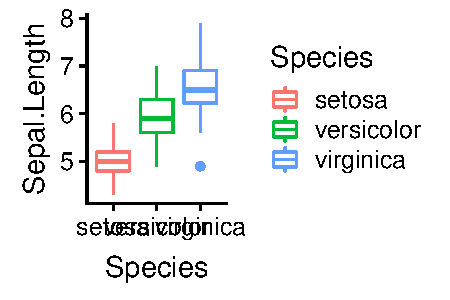
\includegraphics{bookdown-demo_files/figure-latex/unnamed-chunk-139-1.pdf}

\section{Basic boxplot lables}\label{basic-boxplot-lables}

\begin{itemize}
\tightlist
\item
  now use + xlab() and + ylab()
\end{itemize}

\begin{Shaded}
\begin{Highlighting}[]
\KeywordTok{qplot}\NormalTok{(}\DataTypeTok{y =}\NormalTok{ Sepal.Length,}
      \DataTypeTok{x =}\NormalTok{ Species,    }
        \DataTypeTok{data =}\NormalTok{ iris,}
      \DataTypeTok{geom =} \StringTok{"boxplot"}\NormalTok{,}
      \DataTypeTok{color =}\NormalTok{ Species) }\OperatorTok{+}
\StringTok{  }\KeywordTok{xlab}\NormalTok{(}\StringTok{"Iris Species"}\NormalTok{) }\OperatorTok{+}\StringTok{  }
\StringTok{  }\KeywordTok{ylab}\NormalTok{ (}\StringTok{"Sepal Length (mm)"}\NormalTok{)}
\end{Highlighting}
\end{Shaded}

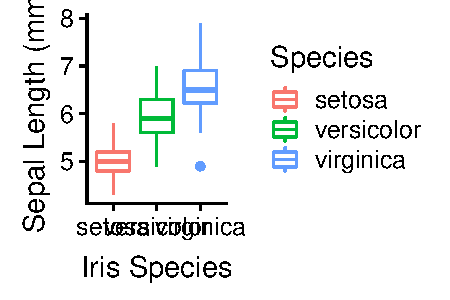
\includegraphics{bookdown-demo_files/figure-latex/unnamed-chunk-140-1.pdf}

\section{Histograms using qplot}\label{histograms-using-qplot}

\begin{itemize}
\tightlist
\item
  made with geom = ``histogram'' arguement
\item
  very very easy to make in R with ggplot
\item
  very very very hard to make in Excel
\item
  You should make them all the time for you data!
\end{itemize}

\subsection{Histograms of iris data}\label{histograms-of-iris-data}

\begin{itemize}
\tightlist
\item
  This code makes a histogram of one of the iris species' Petal.Length.
\item
  Note that you don't have ``y ='' or ``x ='' for a histogram!
\end{itemize}

\begin{Shaded}
\begin{Highlighting}[]
\KeywordTok{qplot}\NormalTok{(Petal.Length,}
      \DataTypeTok{data =}\NormalTok{ iris)}
\end{Highlighting}
\end{Shaded}

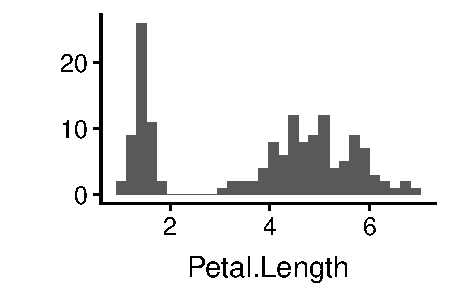
\includegraphics{bookdown-demo_files/figure-latex/unnamed-chunk-141-1.pdf}

\subsection{Histogram with colors}\label{histogram-with-colors}

What does this show?

\begin{Shaded}
\begin{Highlighting}[]
\KeywordTok{qplot}\NormalTok{(Petal.Length,}
      \DataTypeTok{data =}\NormalTok{ iris,}
      \DataTypeTok{fill =}\NormalTok{ Species)}
\end{Highlighting}
\end{Shaded}

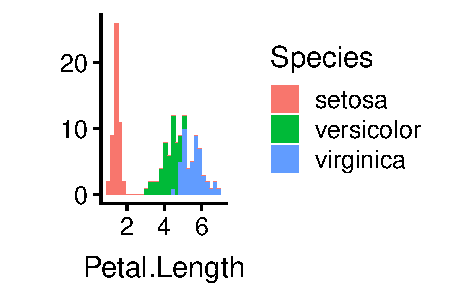
\includegraphics{bookdown-demo_files/figure-latex/unnamed-chunk-142-1.pdf}

\subsection{Histogram with axes
labels}\label{histogram-with-axes-labels}

\begin{Shaded}
\begin{Highlighting}[]
\KeywordTok{qplot}\NormalTok{(Petal.Length,}
      \DataTypeTok{data =}\NormalTok{ iris,}
      \DataTypeTok{fill =}\NormalTok{ Species) }\OperatorTok{+}\StringTok{  }
\StringTok{  }\KeywordTok{xlab}\NormalTok{ (}\StringTok{"Sepal Length (mm)"}\NormalTok{)}
\end{Highlighting}
\end{Shaded}

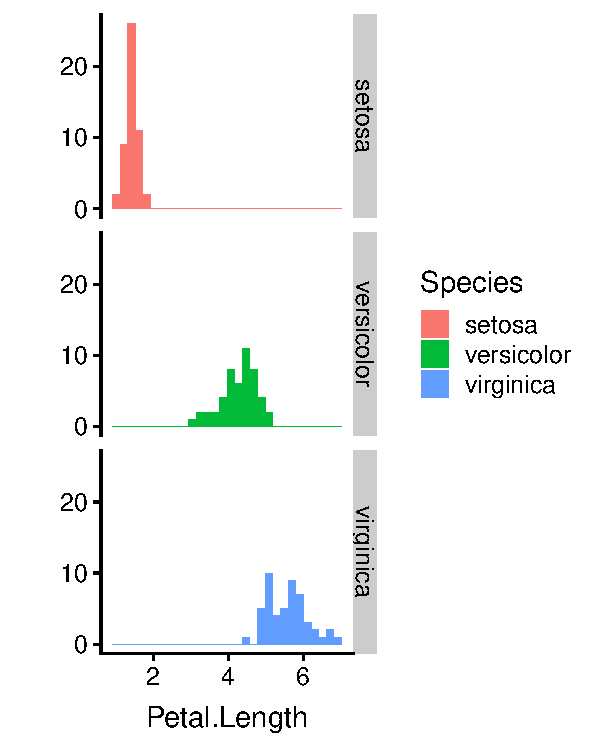
\includegraphics{bookdown-demo_files/figure-latex/unnamed-chunk-143-1.pdf}

\subsection{\texorpdfstring{Multiple histograms:
``Facets''}{Multiple histograms: Facets}}\label{multiple-histograms-facets}

What does this show?

\begin{Shaded}
\begin{Highlighting}[]
\KeywordTok{qplot}\NormalTok{(Petal.Length,}
      \DataTypeTok{data =}\NormalTok{ iris,}
      \DataTypeTok{fill =}\NormalTok{ Species,}
      \DataTypeTok{facets =}\NormalTok{ Species }\OperatorTok{~}\NormalTok{.) }
\end{Highlighting}
\end{Shaded}

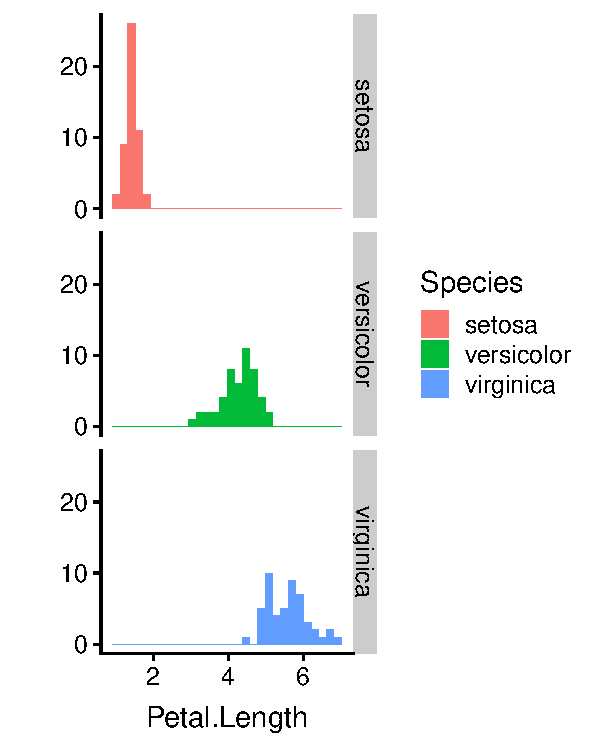
\includegraphics{bookdown-demo_files/figure-latex/unnamed-chunk-144-1.pdf}

Add a label to x-axis

\begin{Shaded}
\begin{Highlighting}[]
\KeywordTok{qplot}\NormalTok{(Petal.Length,}
      \DataTypeTok{data =}\NormalTok{ iris,}
      \DataTypeTok{fill =}\NormalTok{ Species,}
      \DataTypeTok{facets =}\NormalTok{ Species }\OperatorTok{~}\NormalTok{.) }\OperatorTok{+}\StringTok{  }
\StringTok{  }\KeywordTok{xlab}\NormalTok{(}\StringTok{"Sepal Length (mm)"}\NormalTok{)}
\end{Highlighting}
\end{Shaded}

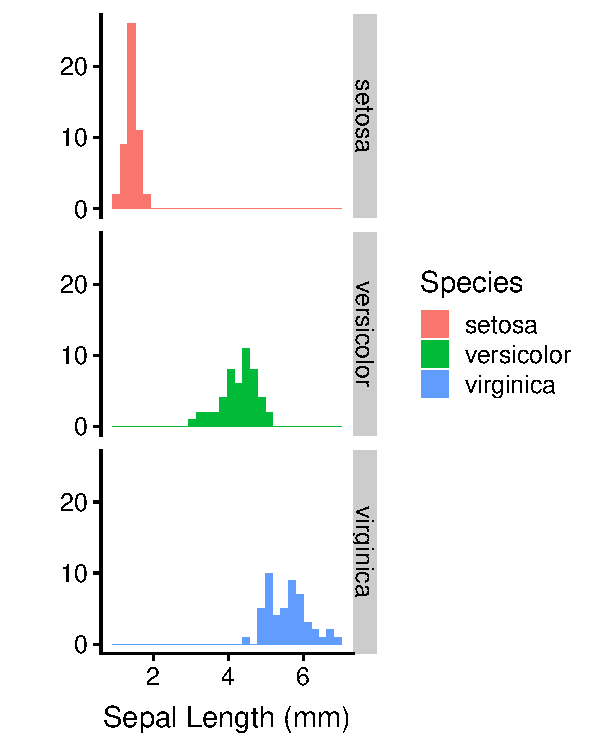
\includegraphics{bookdown-demo_files/figure-latex/unnamed-chunk-145-1.pdf}

\section{Modifying histograms: titles with the main =
argument}\label{modifying-histograms-titles-with-the-main-argument}

\begin{itemize}
\tightlist
\item
  Titles are good for your own personal use but actually are almost
  never used in figures published in papers and books.
\item
  We can add a title like this using the arguement ``main =''
\end{itemize}

\begin{Shaded}
\begin{Highlighting}[]
\KeywordTok{qplot}\NormalTok{(Petal.Length,}
      \DataTypeTok{data =}\NormalTok{ iris,}
      \DataTypeTok{fill =}\NormalTok{ Species,}
      \DataTypeTok{main =} \StringTok{"Iris species histograms"}\NormalTok{,}
      \DataTypeTok{facets =}\NormalTok{ Species }\OperatorTok{~}\NormalTok{.) }\OperatorTok{+}\StringTok{  }
\StringTok{  }\KeywordTok{xlab}\NormalTok{ (}\StringTok{"Sepal Length (mm)"}\NormalTok{)}
\end{Highlighting}
\end{Shaded}

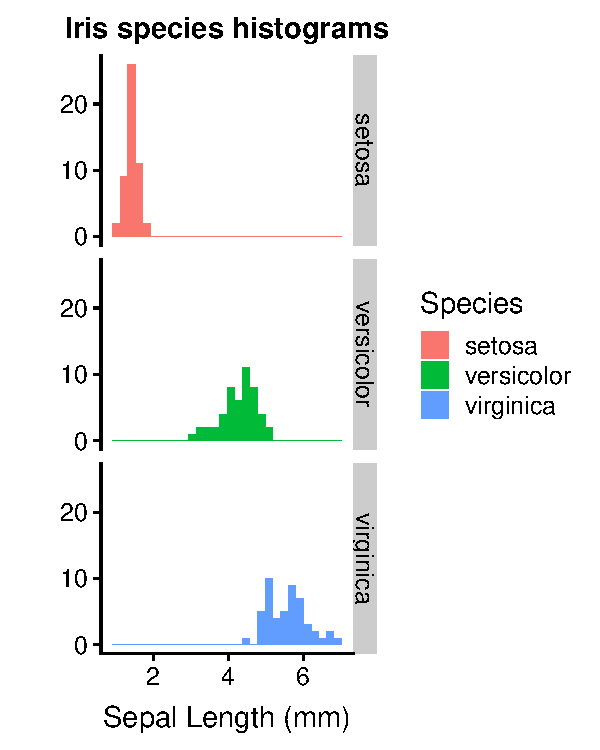
\includegraphics{bookdown-demo_files/figure-latex/last.chunk.sxn3.ch2-1.pdf}

\section{Challenge: Make a histogram of the mammals
data}\label{challenge-make-a-histogram-of-the-mammals-data}

\begin{itemize}
\tightlist
\item
  Load the MASS library using library(MASS)
\item
  Load the mammals data using data(mammals)
\item
  Make a histogram of the log of body mass
\item
  Add labels using xlab() and ylab()
\end{itemize}

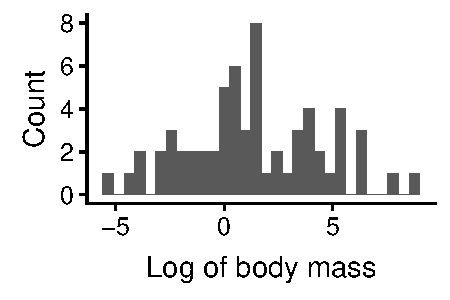
\includegraphics{bookdown-demo_files/figure-latex/unnamed-chunk-146-1.pdf}

\chapter{Scatterplots in R Using
qplot()}\label{scatterplots-in-r-using-qplot}

\textbf{Nathan Brouwer, Phd}\\
brouwern at gmail.com\\
\url{https://github.com/brouwern}\\
Twitter: lobrowR

\section{Introduction}\label{introduction-7}

We'll show how to make \textbf{scatterplots} using the ``quick plot''
function (\textbf{qplot}) from ggplot2. ggplot2::qplot and ggpubr both
offer simplified plotting using tools from ggplot2's toolkit. ggpubr
implements a different syntax, though, while qplot use more standard
ggplot2 idioms and so is a good way to get a sense for the full power of
ggploting.

\subsection*{Learning goals \&
outcomes}\label{learning-goals-outcomes-2}
\addcontentsline{toc}{subsection}{Learning goals \& outcomes}

\begin{itemize}
\tightlist
\item
  Make scatter plots : )
\end{itemize}

\subsection*{Functions \& Arguements}\label{functions-arguements-5}
\addcontentsline{toc}{subsection}{Functions \& Arguements}

\begin{itemize}
\tightlist
\item
  library
\item
  names
\item
  qplot
\item
  data
\item
  dim
\item
  head
\item
  summary
\item
  factor
\item
  log
\end{itemize}

\subsection*{Packages}\label{packages-6}
\addcontentsline{toc}{subsection}{Packages}

\begin{itemize}
\tightlist
\item
  ggplot2
\item
  cowplot
\end{itemize}

\subsection*{Potential hangups}\label{potential-hangups-4}
\addcontentsline{toc}{subsection}{Potential hangups}

There are many ways to make plots in R: ggplot, qplot, ggpubr, plot; and
I'm leaving a few out. Moving between them is meant to give you a sense
for the different tools so you can recognize them ``in the wild'' on the
internet and in books. We'll transition to focusing on ggpubr soon.

\section{Scatterplots: 2 Continuous
Variables}\label{scatterplots-2-continuous-variables}

In this lab we'll explore how to make scatterplots using the qplot()
function in ggplot2.

\subsection{R Preliminaries}\label{r-preliminaries}

\begin{itemize}
\tightlist
\item
  We'll use the qplot() function in the \emph{ggplot} package
\item
  The \emph{cowplot} package provides nice deafults for ggplot IMHO
\end{itemize}

\subsection{Scatterplot of Iris data}\label{scatterplot-of-iris-data}

\begin{itemize}
\tightlist
\item
  Let's make a scatter plot, where we plot two continous, numeric
  variables against each other
\item
  that is, both x and y variables are numbers; not categories
\end{itemize}

I've forgotten the names of all the iris variables, so I'll use the
\textbf{names()} command to see what they are

\begin{Shaded}
\begin{Highlighting}[]
\KeywordTok{names}\NormalTok{(iris)}
\end{Highlighting}
\end{Shaded}

I'll plot the sepals against the petals

\begin{Shaded}
\begin{Highlighting}[]
\KeywordTok{qplot}\NormalTok{(}\DataTypeTok{y =}\NormalTok{ Sepal.Length,}
      \DataTypeTok{x =}\NormalTok{ Petal.Length, }
      \DataTypeTok{data =}\NormalTok{ iris)}
\end{Highlighting}
\end{Shaded}

\begin{figure}
\centering
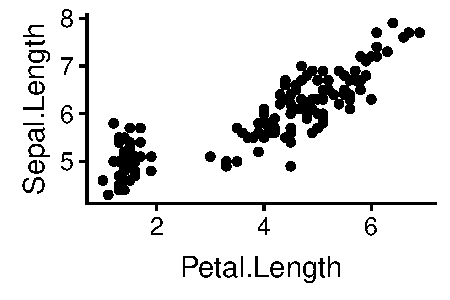
\includegraphics{bookdown-demo_files/figure-latex/unnamed-chunk-148-1.pdf}
\caption{\label{fig:unnamed-chunk-148}Sepals vs.~Petals}
\end{figure}

\subsection{Scatter plot of mammal brain
data}\label{scatter-plot-of-mammal-brain-data}

Let's look at another dataset

\subsubsection{Preliminaries}\label{preliminaries}

Get the data from the ggplot2 package

\begin{Shaded}
\begin{Highlighting}[]
\KeywordTok{data}\NormalTok{(msleep)}
\end{Highlighting}
\end{Shaded}

\subsubsection{Look at the data}\label{look-at-the-data}

\begin{Shaded}
\begin{Highlighting}[]
\KeywordTok{dim}\NormalTok{(msleep) }\CommentTok{#How much data is there?}

\KeywordTok{head}\NormalTok{(msleep) }\CommentTok{#What does the data look like}

\KeywordTok{summary}\NormalTok{(msleep) }\CommentTok{#Summary of the data}
\end{Highlighting}
\end{Shaded}

There are a number of ``categorical'' varibles in this dataset

\begin{itemize}
\tightlist
\item
  genus
\item
  vore = carnivore, omnivore et
\item
  order = taxonomic order
\item
  conservation = conservation status (endangered, etc)
\end{itemize}

For some reason they don't load as ``factor'' variables (better known as
categorical or grouping variables, but called ``Factors'' in R-land)

We can make these factors using the factor() command

\begin{Shaded}
\begin{Highlighting}[]
\NormalTok{msleep}\OperatorTok{$}\NormalTok{vore <-}\StringTok{ }\KeywordTok{factor}\NormalTok{(msleep}\OperatorTok{$}\NormalTok{vore)}
\end{Highlighting}
\end{Shaded}

Now see what happens when you call summary()

\begin{Shaded}
\begin{Highlighting}[]
\KeywordTok{summary}\NormalTok{(msleep)}
\end{Highlighting}
\end{Shaded}

Do the same for ``order''"

\begin{Shaded}
\begin{Highlighting}[]
\NormalTok{msleep}\OperatorTok{$}\NormalTok{order <-}\StringTok{ }\KeywordTok{factor}\NormalTok{(msleep}\OperatorTok{$}\NormalTok{order)}

\KeywordTok{summary}\NormalTok{(msleep)}
\end{Highlighting}
\end{Shaded}

And ``conservation''

\begin{Shaded}
\begin{Highlighting}[]
\NormalTok{msleep}\OperatorTok{$}\NormalTok{conservation <-}\StringTok{ }\KeywordTok{factor}\NormalTok{(msleep}\OperatorTok{$}\NormalTok{conservation)}

\KeywordTok{summary}\NormalTok{(msleep)}
\end{Highlighting}
\end{Shaded}

\subsection{Make a basic scatterplot}\label{make-a-basic-scatterplot}

\begin{Shaded}
\begin{Highlighting}[]
\KeywordTok{qplot}\NormalTok{(}\DataTypeTok{y =}\NormalTok{ sleep_total,}
      \DataTypeTok{x =}\NormalTok{ brainwt, }
      \DataTypeTok{data =}\NormalTok{ msleep)}
\end{Highlighting}
\end{Shaded}

\begin{figure}
\centering
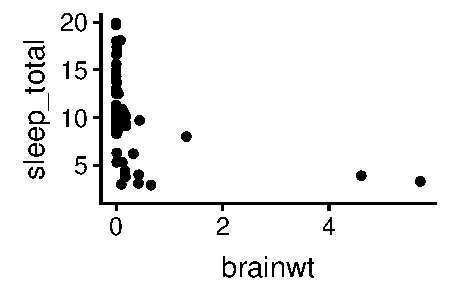
\includegraphics{bookdown-demo_files/figure-latex/unnamed-chunk-155-1.pdf}
\caption{\label{fig:unnamed-chunk-155}Mammal sleep, raw data}
\end{figure}

That looks really really ugly. It will work better if we ``log transform
the axes''

\begin{Shaded}
\begin{Highlighting}[]
\KeywordTok{qplot}\NormalTok{(}\DataTypeTok{y =} \KeywordTok{log}\NormalTok{(sleep_rem),}
      \DataTypeTok{x =} \KeywordTok{log}\NormalTok{(brainwt), }
      \DataTypeTok{data =}\NormalTok{ msleep)}
\end{Highlighting}
\end{Shaded}

\begin{figure}
\centering
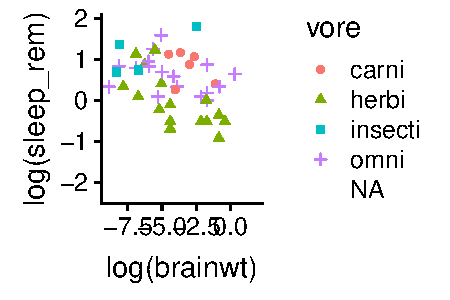
\includegraphics{bookdown-demo_files/figure-latex/unnamed-chunk-156-1.pdf}
\caption{\label{fig:unnamed-chunk-156}Mammal sleep, logged data}
\end{figure}

Things get logged all the time in stats. We'll talk more about that
later.

\subsection{Add color coding to
scatterplot}\label{add-color-coding-to-scatterplot}

\begin{Shaded}
\begin{Highlighting}[]
\KeywordTok{qplot}\NormalTok{(}\DataTypeTok{y =} \KeywordTok{log}\NormalTok{(sleep_rem),}
      \DataTypeTok{x =} \KeywordTok{log}\NormalTok{(brainwt), }
      \DataTypeTok{data =}\NormalTok{ msleep,}
      \DataTypeTok{color =}\NormalTok{ vore)}
\end{Highlighting}
\end{Shaded}

\begin{figure}
\centering
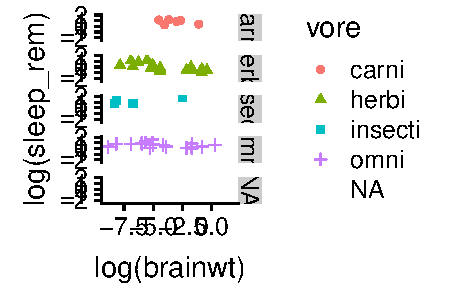
\includegraphics{bookdown-demo_files/figure-latex/unnamed-chunk-157-1.pdf}
\caption{\label{fig:unnamed-chunk-157}Add colors with color =}
\end{figure}

\subsection{Add color \& shape coding to
scatterplot}\label{add-color-shape-coding-to-scatterplot}

\begin{Shaded}
\begin{Highlighting}[]
\KeywordTok{qplot}\NormalTok{(}\DataTypeTok{y =} \KeywordTok{log}\NormalTok{(sleep_rem),}
      \DataTypeTok{x =} \KeywordTok{log}\NormalTok{(brainwt), }
      \DataTypeTok{data =}\NormalTok{ msleep,}
      \DataTypeTok{color =}\NormalTok{ vore,}
      \DataTypeTok{shape =}\NormalTok{ vore)}
\end{Highlighting}
\end{Shaded}

\begin{figure}
\centering
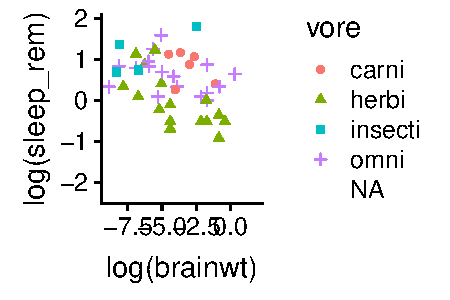
\includegraphics{bookdown-demo_files/figure-latex/unnamed-chunk-158-1.pdf}
\caption{\label{fig:unnamed-chunk-158}Add shapes with shape =}
\end{figure}

\subsection{\texorpdfstring{Put diffetrent ``vores'' in seperate
panels}{Put diffetrent vores in seperate panels}}\label{put-diffetrent-vores-in-seperate-panels}

\begin{itemize}
\tightlist
\item
  Seperate panels can be made using the ``facet'' arguement withing
  qplot
\end{itemize}

\begin{Shaded}
\begin{Highlighting}[]
\KeywordTok{qplot}\NormalTok{(}\DataTypeTok{y =} \KeywordTok{log}\NormalTok{(sleep_rem),}
      \DataTypeTok{x =} \KeywordTok{log}\NormalTok{(brainwt), }
      \DataTypeTok{data =}\NormalTok{ msleep,}
      \DataTypeTok{color =}\NormalTok{ vore,}
      \DataTypeTok{shape =}\NormalTok{ vore,}
      \DataTypeTok{facets =}\NormalTok{ vore }\OperatorTok{~}\StringTok{ }\NormalTok{.)}
\end{Highlighting}
\end{Shaded}

\begin{figure}
\centering
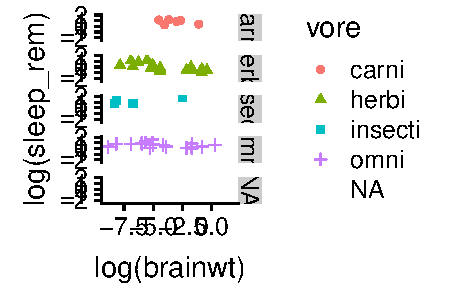
\includegraphics{bookdown-demo_files/figure-latex/unnamed-chunk-159-1.pdf}
\caption{\label{fig:unnamed-chunk-159}Split into different panels w/ facets
=}
\end{figure}

\subsection{\texorpdfstring{Add a ``trend line''" to a
scatterplot}{Add a trend line" to a scatterplot}}\label{add-a-trend-line-to-a-scatterplot}

\begin{itemize}
\tightlist
\item
  Add the geom\_smooth() function after the initial qplot() command
\item
  This works best if we remove the ``color = vore'' command, but you can
  see what happens if you leave it
\end{itemize}

\begin{Shaded}
\begin{Highlighting}[]
\KeywordTok{qplot}\NormalTok{(}\DataTypeTok{y =} \KeywordTok{log}\NormalTok{(sleep_rem),}
      \DataTypeTok{x =} \KeywordTok{log}\NormalTok{(brainwt), }
      \DataTypeTok{data =}\NormalTok{ msleep) }\OperatorTok{+}
\StringTok{  }\KeywordTok{geom_smooth}\NormalTok{()}
\end{Highlighting}
\end{Shaded}

\begin{figure}
\centering
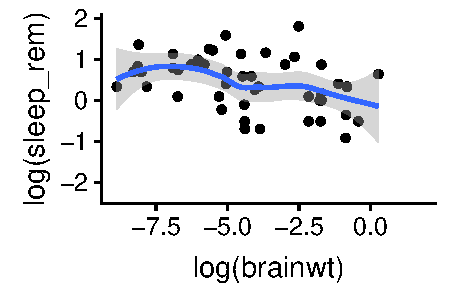
\includegraphics{bookdown-demo_files/figure-latex/last.chnk.sxn3.ch3-1.pdf}
\caption{(\#fig:last.chnk.sxn3.ch3)Add trendline with + geom\_smooth()}
\end{figure}

\subsection{Challenge: Modify mammal brain
code}\label{challenge-modify-mammal-brain-code}

Modify the mamal bran code to do the following things

\begin{itemize}
\tightlist
\item
  Change the axes labels (eg ``+ ylab(`y axis')'')
\item
  Add a title (eg " + ggtitle(`\ldots{}')``)
\item
  Use names(msleep) to see what other varibles are in the dataset
\item
  Use summary(msleep) to whether they are continous or categorical
\item
  Pick another continous variable and plot it instead of sleep\_total
\item
  Try this with and without logging using the log() command
\end{itemize}

\part{Data analysis: a first
encounter}\label{part-data-analysis-a-first-encounter}

\hypertarget{section-3}{\subsection*{}\label{section-3}}
\addcontentsline{toc}{subsection}{}

In this section we will tackle a typical data analysis problem:
determining if two groups of organisms an be considering statistically
differnet from each other. We will use data from a paper titled ``Sperm
competition and the evolution of precopulatory weapons: Increasing male
density promotes sperm competition and reduces selection on arm strength
in a chorusing frog'' by Buzatto et al (2015). The end goal is to
compare the size of the arms on female and male frogs. First, though, we
will get to know the data by calcualting summary statistics and making
exploratory graphs. We will then carry out a t-test and grabble with
with the meaning and interpretation of the output is. Finally, we'll
explore how best to plot the output of your t-test.

\begin{enumerate}
\def\labelenumi{\arabic{enumi}.}
\tightlist
\item
  Data exploration with summary statistics
\item
  Graphical data exploration
\item
  Plotting means and measures of variation and precisions
\item
  T-test
\item
  Plotting the output of a t-test
\end{enumerate}

\chapter{Data Analysis Encounter: Summary
Statistics}\label{data-analysis-encounter-summary-statistics}

\textbf{Nathan Brouwer, Phd}\\
brouwern at gmail.com\\
\url{https://github.com/brouwern}\\
Twitter: lobrowR

\section{Introduction}\label{introduction-8}

\subsection{Goals and objectives}\label{goals-and-objectives}

Get to know the frogarms dataset and learn how to calculat summary
statistics using basic R functions (eg summary() ) and also with dplyr.

\subsection{Outline}\label{outline-2}

\begin{enumerate}
\def\labelenumi{\arabic{enumi}.}
\tightlist
\item
  Load packages and data
\item
  Subset data
\item
  Calculate summary stats on columns
\item
  Use dplyr
\item
  Calcualte summary stats by group using
\end{enumerate}

\subsection{Packages}\label{packages-7}

\begin{itemize}
\tightlist
\item
  devtools
\item
  wildlifeR (from GitHub)
\end{itemize}

\subsection{Functions}\label{functions-1}

\begin{itemize}
\tightlist
\item
  devtools::install\_github()
\item
  wildlifeR::make\_my\_data2L
\item
  dim
\item
  nrow
\item
  ncol
\item
  head
\item
  tail
\item
  names
\item
  summary
\item
  median()
\item
  min()
\item
  max()
\item
  var()
\item
  sd()
\item
  range()
\item
  nrow() or length() (for sample size)
\item
  dplyr::summarise(), dplyr::summarize()
\item
  group\_by()
\item
  dplyr::n()
\end{itemize}

\section{Preliminaries}\label{preliminaries-1}

First, we nee to install the necessary packages. The data are in a
package stored on GitHub called wildlifeR. The devtools package is
needed for downloading from github. We'll also use dplyr for grouping
data and calcualting summary statistics.

\subsection{Load packages}\label{load-packages}

You might have to install or re-install wildlifeR using
install.packages()

\begin{Shaded}
\begin{Highlighting}[]
\KeywordTok{library}\NormalTok{(devtools)}
\KeywordTok{install_github}\NormalTok{(}\StringTok{"brouwern/"}\NormalTok{)}
\end{Highlighting}
\end{Shaded}

Recall that downloiading a package and actually loading it into R's
active memory are different things. To actually use the pakcage you need
to use the librar() command

\subsection{Load data}\label{load-data}

The data we'll be using is in a dataset called ``frogarms'' in the
wildlifeR package.

\begin{Shaded}
\begin{Highlighting}[]
\KeywordTok{data}\NormalTok{(frogarms)}
\end{Highlighting}
\end{Shaded}

You can find out information about these data using the ? command. Note
that there are no parenthese required for this.

\subsection{Subset your data}\label{subset-your-data}

The function make\_my\_data2L() in the wildlfieR will extact out a
random subset of the data. Change ``my.code'' to your school email
address, minus the ``\citet{pitt.edu}'' or whatever your affiliation is.

\begin{Shaded}
\begin{Highlighting}[]
\NormalTok{my.frogs <-}\StringTok{ }\NormalTok{frogarms}
\NormalTok{my.frogs <-}\StringTok{ }\KeywordTok{make_my_data2L}\NormalTok{(}\DataTypeTok{dat =}\NormalTok{ frogarms,}
                           \DataTypeTok{my.code =} \StringTok{"nlb24"}\NormalTok{, }\CommentTok{# <=  change this!}
                           \DataTypeTok{cat.var =} \StringTok{"sex"}\NormalTok{,}
                           \DataTypeTok{n.sample =} \DecValTok{20}\NormalTok{,}
                           \DataTypeTok{with.rep =} \OtherTok{FALSE}\NormalTok{)}
\end{Highlighting}
\end{Shaded}

n.sample is set to 20. This is set up to extract 20 unique individuals
of each sex. Check that you dataframe is 2*20 = 40 rows using the dim()
command.

\begin{Shaded}
\begin{Highlighting}[]
\KeywordTok{dim}\NormalTok{(my.frogs)}
\end{Highlighting}
\end{Shaded}

\section{A 1st encounter with R: getting to know your
dataframe}\label{a-1st-encounter-with-r-getting-to-know-your-dataframe}

\subsection{Dataframe dimension}\label{dataframe-dimension}

The following commands tell you the row x column dimension, number of
rows, and number of columns.

\begin{Shaded}
\begin{Highlighting}[]
\KeywordTok{dim}\NormalTok{(my.frogs)}
\KeywordTok{nrow}\NormalTok{(my.frogs)}
\KeywordTok{ncol}\NormalTok{(my.frogs)}
\end{Highlighting}
\end{Shaded}

\begin{center}\rule{0.5\linewidth}{\linethickness}\end{center}

\subsection{Optional: accessing elements of
objects}\label{optional-accessing-elements-of-objects}

The following section is optional.

The commands dim, nrow and ncol all generate objects that display
informatio on the dimension of a dataframe. dim() produces and object
that is a ``vector'' that is 1 row x 2 elemtns in size. We can select
these individual elements using square brackets

The full dim() output

\begin{Shaded}
\begin{Highlighting}[]
\KeywordTok{dim}\NormalTok{(my.frogs)}
\end{Highlighting}
\end{Shaded}

The 1st element of the dim() output

\begin{Shaded}
\begin{Highlighting}[]
\KeywordTok{dim}\NormalTok{(my.frogs)[}\DecValTok{1}\NormalTok{]}
\end{Highlighting}
\end{Shaded}

The 2nd element

\begin{Shaded}
\begin{Highlighting}[]
\KeywordTok{dim}\NormalTok{(my.frogs)[}\DecValTok{2}\NormalTok{]}
\end{Highlighting}
\end{Shaded}

Both elements

\begin{Shaded}
\begin{Highlighting}[]
\KeywordTok{dim}\NormalTok{(my.frogs)[}\DecValTok{1}\OperatorTok{:}\DecValTok{2}\NormalTok{]}
\end{Highlighting}
\end{Shaded}

Another way to get both elements

\begin{Shaded}
\begin{Highlighting}[]
\KeywordTok{dim}\NormalTok{(my.frogs)[}\KeywordTok{c}\NormalTok{(}\DecValTok{1}\NormalTok{,}\DecValTok{2}\NormalTok{)]}
\end{Highlighting}
\end{Shaded}

What happens when you execute this command?

\begin{Shaded}
\begin{Highlighting}[]
\KeywordTok{dim}\NormalTok{(my.frogs)[}\KeywordTok{c}\NormalTok{(}\DecValTok{2}\NormalTok{,}\DecValTok{1}\NormalTok{)]}
\end{Highlighting}
\end{Shaded}

\textbf{End optional section}

\begin{center}\rule{0.5\linewidth}{\linethickness}\end{center}

\subsection{Dataframe preview}\label{dataframe-preview}

The head() and tail() commands give up short previews of the dataframe

The top few rows

\begin{Shaded}
\begin{Highlighting}[]
\KeywordTok{head}\NormalTok{(my.frogs)}
\end{Highlighting}
\end{Shaded}

The bottom few rows

\begin{Shaded}
\begin{Highlighting}[]
\KeywordTok{tail}\NormalTok{(my.frogs)}
\end{Highlighting}
\end{Shaded}

names() just gives of the names

\begin{Shaded}
\begin{Highlighting}[]
\KeywordTok{names}\NormalTok{(my.frogs)}
\end{Highlighting}
\end{Shaded}

Again, if you want ot know what the column names are, use the ? command

\begin{Shaded}
\begin{Highlighting}[]
\NormalTok{?my.frogs}
\end{Highlighting}
\end{Shaded}

\section{A 1st encounter with R: summary
statistics}\label{a-1st-encounter-with-r-summary-statistics}

R is a giant calculater. There are commands for mean, median, standard
deviation etc. The summary() command creates a handy summary of an
entire dataframe.

\subsection{Overall summary}\label{overall-summary}

Whole dataframe

\begin{Shaded}
\begin{Highlighting}[]
\KeywordTok{summary}\NormalTok{(my.frogs)}
\end{Highlighting}
\end{Shaded}

We can look at just a single column by specifying it using the syntax
``dataframe\(column.names" where the dataframe and column are sperated by a dollar sig (\)).
(note that it prints it out horizontally, not vertially)

\begin{Shaded}
\begin{Highlighting}[]
\KeywordTok{summary}\NormalTok{(my.frogs}\OperatorTok{$}\NormalTok{mass)}
\end{Highlighting}
\end{Shaded}

We used the make\_my\_data2L command to make a unique subset of the
data. compare the mass values in your subset to the original data

\begin{Shaded}
\begin{Highlighting}[]
\KeywordTok{summary}\NormalTok{(my.frogs}\OperatorTok{$}\NormalTok{mass)}
\KeywordTok{summary}\NormalTok{(frogarms}\OperatorTok{$}\NormalTok{mass)}
\end{Highlighting}
\end{Shaded}

\begin{center}\rule{0.5\linewidth}{\linethickness}\end{center}

\subsection{Optional: stacking things with
rbind()}\label{optional-stacking-things-with-rbind}

\textbf{This is optional}

Handy trick: stack up the summaries with rbind()

\begin{Shaded}
\begin{Highlighting}[]
\KeywordTok{rbind}\NormalTok{(}\KeywordTok{summary}\NormalTok{(my.frogs}\OperatorTok{$}\NormalTok{mass),}
      \KeywordTok{summary}\NormalTok{(frogarms}\OperatorTok{$}\NormalTok{mass))}
\end{Highlighting}
\end{Shaded}

You can even flip them on their side like this

\begin{Shaded}
\begin{Highlighting}[]
\NormalTok{my.summaries <-}\StringTok{ }\KeywordTok{rbind}\NormalTok{(}\KeywordTok{summary}\NormalTok{(my.frogs}\OperatorTok{$}\NormalTok{mass),}
                      \KeywordTok{summary}\NormalTok{(frogarms}\OperatorTok{$}\NormalTok{mass))}
\end{Highlighting}
\end{Shaded}

\begin{Shaded}
\begin{Highlighting}[]
\KeywordTok{t}\NormalTok{(my.summaries)}
\end{Highlighting}
\end{Shaded}

\textbf{End optional section}

\begin{center}\rule{0.5\linewidth}{\linethickness}\end{center}

\subsection{Individual summary stats}\label{individual-summary-stats}

You can get individual summary statistics using various commands named
after the statistic

The mean of a coulumn

\begin{Shaded}
\begin{Highlighting}[]
\KeywordTok{mean}\NormalTok{(my.frogs}\OperatorTok{$}\NormalTok{mass)}
\end{Highlighting}
\end{Shaded}

The variance

\begin{Shaded}
\begin{Highlighting}[]
\KeywordTok{var}\NormalTok{(my.frogs}\OperatorTok{$}\NormalTok{mass)}
\end{Highlighting}
\end{Shaded}

Other include:

\begin{itemize}
\tightlist
\item
  median()
\item
  min()
\item
  max()
\item
  var()
\item
  sd()
\item
  range()
\item
  nrow() or length() (for sample size)
\end{itemize}

Note that range() returns two values in a vector

\begin{Shaded}
\begin{Highlighting}[]
\KeywordTok{range}\NormalTok{(my.frogs}\OperatorTok{$}\NormalTok{mass)}
\end{Highlighting}
\end{Shaded}

\subsection{The standard error (SE) in
R}\label{the-standard-error-se-in-r}

Note that R doesn't return a very common statistic, the standard error
(SE). The SE is the standard deviation (SD) deivided by the square root
of the sample size. You can get the same size using the length()
command.

You can therefore calcualte the SE like this:

\begin{Shaded}
\begin{Highlighting}[]
\KeywordTok{sd}\NormalTok{(my.frogs}\OperatorTok{$}\NormalTok{mass)}\OperatorTok{/}\KeywordTok{sqrt}\NormalTok{(}\KeywordTok{length}\NormalTok{(my.frogs}\OperatorTok{$}\NormalTok{mass))}
\end{Highlighting}
\end{Shaded}

\begin{center}\rule{0.5\linewidth}{\linethickness}\end{center}

In the following two optional sections you can

\begin{itemize}
\tightlist
\item
  try to find a package with an SE fucntion
\item
  try to write a function that calcualtes the SE for you
\end{itemize}

\subsection{OPTIONAL: Find a package the calcualtes the
SE}\label{optional-find-a-package-the-calcualtes-the-se}

Since R lacks a an SE function many packages include it. For example,
the plotrix package has a function std.error(). See if you can download
the package, install it using library(), and use the std.error(). See
the help package for more info (?std.error)

\subsection{OPTIONAL: Write your own SD
function}\label{optional-write-your-own-sd-function}

Write a function for calculationg the SD

Here's a function that takes a single arguement ``dat\_column''

\begin{Shaded}
\begin{Highlighting}[]
\CommentTok{#NOTE: this is optional}
\NormalTok{my_sd1 <-}\StringTok{ }\ControlFlowTok{function}\NormalTok{(dat_column)\{}
  \KeywordTok{sd}\NormalTok{(dat_column)}\OperatorTok{/}\KeywordTok{sqrt}\NormalTok{(}\KeywordTok{length}\NormalTok{(dat_column))}
\NormalTok{\}}
\end{Highlighting}
\end{Shaded}

To use it, you need to give it the dataframe and the column seperated by
a \$

\begin{Shaded}
\begin{Highlighting}[]
\KeywordTok{my_sd1}\NormalTok{(my.frogs}\OperatorTok{$}\NormalTok{mass)}
\end{Highlighting}
\end{Shaded}

Here's a function that takes 2 arguements: the dataframe, and the name
of the column Note that the name of the column needs to be in quotes

\begin{Shaded}
\begin{Highlighting}[]
\NormalTok{my_sd2 <-}\StringTok{ }\ControlFlowTok{function}\NormalTok{(dat, column)\{}
  \KeywordTok{sd}\NormalTok{(dat[,column])}\OperatorTok{/}\KeywordTok{sqrt}\NormalTok{(}\KeywordTok{length}\NormalTok{(dat[,column]))}
\NormalTok{\}}
\end{Highlighting}
\end{Shaded}

You can use the function like this:

\begin{Shaded}
\begin{Highlighting}[]
\KeywordTok{my_sd2}\NormalTok{(my.frogs, }\StringTok{"mass"}\NormalTok{)}
\end{Highlighting}
\end{Shaded}

Here's a fancier function that let's you specify how much to round off
the results. I've set the default rounding to 3 digits.

\begin{Shaded}
\begin{Highlighting}[]
\NormalTok{my_sd3 <-}\StringTok{ }\ControlFlowTok{function}\NormalTok{(dat, column, }\DataTypeTok{digits.round =} \DecValTok{3}\NormalTok{)\{}
\NormalTok{  se <-}\StringTok{ }\KeywordTok{sd}\NormalTok{(dat[,column])}\OperatorTok{/}\KeywordTok{sqrt}\NormalTok{(}\KeywordTok{length}\NormalTok{(dat[,column]))}
  \KeywordTok{round}\NormalTok{(se, }\DataTypeTok{digits =}\NormalTok{ digits.round)}
\NormalTok{\}}
\end{Highlighting}
\end{Shaded}

The function runs like this.

\begin{Shaded}
\begin{Highlighting}[]
\KeywordTok{my_sd3}\NormalTok{(my.frogs, }\StringTok{"mass"}\NormalTok{)}
\end{Highlighting}
\end{Shaded}

Note that in all of functions as long as I give the function the
arguements in the same order they are set up in the code that defines
the function, I don't need to provide the names. This save typing.
Compare these results

\textbf{End optional section}

\begin{center}\rule{0.5\linewidth}{\linethickness}\end{center}

\section{A 1st encounter with dplyr}\label{a-1st-encounter-with-dplyr}

dplyr is a package that provides numerous functions for manipulating
data. We will use two handy functions

\begin{itemize}
\tightlist
\item
  summarize() / summarise()
\item
  group\_by()
\end{itemize}

dplyr can use a handy sytax that involes ``pipes''. You can string
together R commands using the pipe function \%\textgreater{}\%

When using pipes, you start with a dataframe and follow it with an
action you want done to it. So, for example, previously when we wanted
the mean of the ``mass''" column we did this

\begin{Shaded}
\begin{Highlighting}[]
\KeywordTok{mean}\NormalTok{(my.frogs}\OperatorTok{$}\NormalTok{mass)}
\end{Highlighting}
\end{Shaded}

Which is kind of read like a normal mathematical equation or function,
where you start from inside the parentheses and work out.

Eg, this.is.read.2nd(this.is.read.1st)

R let's you nest as many functions as you wnat. If i want to round the
wrap ``mean(my.frogs\$mass)'' in ``round(\ldots{})''"

\begin{Shaded}
\begin{Highlighting}[]
\KeywordTok{round}\NormalTok{(}\KeywordTok{mean}\NormalTok{(my.frogs}\OperatorTok{$}\NormalTok{mass))}
\end{Highlighting}
\end{Shaded}

Using pipes to get the mean I write things more like a sentence

Eg, this.is.read.1st \%\textgreater{}\% this.is.read.2nd

\begin{Shaded}
\begin{Highlighting}[]
\NormalTok{my.frogs}\OperatorTok{$}\NormalTok{mass }\OperatorTok\StringTok{ }\NormalTok{mean }\CommentTok{#note parentheses after mean!}
\end{Highlighting}
\end{Shaded}

Which reads kind of like ``Take the mass column and the datagrame and
apply the mean() function to it.''

To round the mean we would do this

\begin{Shaded}
\begin{Highlighting}[]
\NormalTok{my.frogs}\OperatorTok{$}\NormalTok{mass }\OperatorTok\StringTok{ }\NormalTok{mean }\OperatorTok\StringTok{ }\NormalTok{round}
\end{Highlighting}
\end{Shaded}

Which read left to right like a sentence is ``Take the mass column,
calcualte the mean and then round it.''

Note that the rond() command has an arguement for how many digits you
want to round to. You include that in the parantehes

\begin{Shaded}
\begin{Highlighting}[]
\NormalTok{my.frogs}\OperatorTok{$}\NormalTok{mass }\OperatorTok\StringTok{ }\KeywordTok{mean}\NormalTok{() }\OperatorTok\StringTok{ }\KeywordTok{round}\NormalTok{(}\DataTypeTok{digits =} \DecValTok{2}\NormalTok{)}
\end{Highlighting}
\end{Shaded}

\subsubsection{dplyr's summarize()
command}\label{dplyrs-summarize-command}

Instead of mean(data\$column) we can use summarise() (for the British)
or summarize(), plus pipes.

We can get the grand mean of just the mass column by loading dplyr using
library() and then using the summarise() commnad

\begin{Shaded}
\begin{Highlighting}[]
\KeywordTok{library}\NormalTok{(dplyr)}
\NormalTok{my.frogs }\OperatorTok\StringTok{ }\KeywordTok{summarise}\NormalTok{(}\KeywordTok{mean}\NormalTok{(mass))}
\end{Highlighting}
\end{Shaded}

This is maybe more complicated than
``mean(my.frogs\(mass)" or my.frogs\)mass \%\textgreater{}\% mean, but
overall the pipe framework and summarise pays off when combined with
group\_by() in the next section

\section{dplyr's group\_by() function}\label{dplyrs-group_by-function}

For some more info on group\_by see

\begin{itemize}
\tightlist
\item
  \url{https://www.r-bloggers.com/using-r-quickly-calculating-summary-statistics-with-dplyr/}
\item
  \url{https://www3.nd.edu/~steve/computing_with_data/24_dplyr/dplyr.html}
  \url{http://www.datacarpentry.org/R-genomics/04-dplyr.html}
\end{itemize}

We can use group\_by() to split things up by a categorical variable
(sex, color, year). Here, we can say ``take my.frogs, split up the data
by the sex column, and apply the mean() function to each subset.''

\begin{Shaded}
\begin{Highlighting}[]
\NormalTok{my.frogs }\OperatorTok\StringTok{            }\CommentTok{#the data}
\StringTok{  }\KeywordTok{group_by}\NormalTok{(sex) }\OperatorTok\StringTok{     }\CommentTok{#the group_by() function applied to the sex column}
\StringTok{  }\KeywordTok{summarise}\NormalTok{(}\KeywordTok{mean}\NormalTok{(mass)) }\CommentTok{#the mean() function, applied to mass.}
\end{Highlighting}
\end{Shaded}

This might be a bit abstract when you first do it. Again, where starting
with our whole datefarme, then its piped over to group\_by(), which
splits it essentially into a male and a female subset. Then the mean()
function is applied to each of these subsets.

Note that the column heading in the output \texttt{mean(mass)}, which is
what is in summarise().

A handy thing about summarise is you can pass it lables. The following
code adds a sensible lable by changing ``summarise(mean(mass))'' to
``summarise(mass.mean = mean(mass))'', where ``mass.mean = \ldots{}''
defines the label.

\begin{Shaded}
\begin{Highlighting}[]
\NormalTok{my.frogs }\OperatorTok\StringTok{ }
\StringTok{  }\KeywordTok{group_by}\NormalTok{(sex) }\OperatorTok
\StringTok{  }\KeywordTok{summarise}\NormalTok{(}\DataTypeTok{mass.mean =} \KeywordTok{mean}\NormalTok{(mass))}
\end{Highlighting}
\end{Shaded}

You can lable things anything, eg ``puppies''.

\begin{Shaded}
\begin{Highlighting}[]
\NormalTok{my.frogs }\OperatorTok\StringTok{ }
\StringTok{  }\KeywordTok{group_by}\NormalTok{(sex) }\OperatorTok
\StringTok{  }\KeywordTok{summarise}\NormalTok{(}\DataTypeTok{puppies =} \KeywordTok{mean}\NormalTok{(mass))}
\end{Highlighting}
\end{Shaded}

You can pass any summary function to summarise(). We can give it sd() to
get the sd of mass by sex. Note that I define the column names using
``mass.sd = \ldots{}''

\begin{Shaded}
\begin{Highlighting}[]
\NormalTok{my.frogs }\OperatorTok\StringTok{ }
\StringTok{  }\KeywordTok{group_by}\NormalTok{(sex) }\OperatorTok
\StringTok{  }\KeywordTok{summarise}\NormalTok{(}\DataTypeTok{mass.sd =} \KeywordTok{sd}\NormalTok{(mass))}
\end{Highlighting}
\end{Shaded}

What makes dplyr::group\_by and summarize() really powerful is that you
can pass it \emph{multiple}. summary functions at the same time. Here,
I'll pass mean() and sd(), naming both.

\begin{Shaded}
\begin{Highlighting}[]
\NormalTok{my.frogs }\OperatorTok\StringTok{ }
\StringTok{  }\KeywordTok{group_by}\NormalTok{(sex) }\OperatorTok
\StringTok{  }\KeywordTok{summarise}\NormalTok{(}\DataTypeTok{mass.mean =} \KeywordTok{mean}\NormalTok{(mass),}
            \DataTypeTok{mass.sd =} \KeywordTok{sd}\NormalTok{(mass))}
\end{Highlighting}
\end{Shaded}

dplyr also has a handy function n() for getting your sample size.

\begin{Shaded}
\begin{Highlighting}[]
\NormalTok{my.frogs }\OperatorTok\StringTok{ }
\StringTok{  }\KeywordTok{group_by}\NormalTok{(sex) }\OperatorTok
\StringTok{  }\KeywordTok{summarise}\NormalTok{(}\DataTypeTok{mass.mean =} \KeywordTok{mean}\NormalTok{(mass),}
            \DataTypeTok{mass.sd =} \KeywordTok{sd}\NormalTok{(mass),}
            \DataTypeTok{n =} \KeywordTok{n}\NormalTok{())}
\end{Highlighting}
\end{Shaded}

\begin{center}\rule{0.5\linewidth}{\linethickness}\end{center}

\subsection{OPTIONAL: Using novel function with
dplyr}\label{optional-using-novel-function-with-dplyr}

\textbf{This section is optional}

If you have defined the my\_sd1() function above you can pass it to
summarise() too.

\begin{Shaded}
\begin{Highlighting}[]
\NormalTok{my.frogs }\OperatorTok\StringTok{ }
\StringTok{  }\KeywordTok{group_by}\NormalTok{(sex) }\OperatorTok
\StringTok{  }\KeywordTok{summarise}\NormalTok{(}\DataTypeTok{mass.mean =}  \KeywordTok{my_sd1}\NormalTok{(mass))}
\end{Highlighting}
\end{Shaded}

\textbf{End optional section}

\begin{center}\rule{0.5\linewidth}{\linethickness}\end{center}

\begin{center}\rule{0.5\linewidth}{\linethickness}\end{center}

\section{OPTIONAL: ALternatives to
dplyr}\label{optional-alternatives-to-dplyr}

\textbf{This section is optional}

Most everybody is switching to dplyr. Below are some other idioms you
may see others use or encouter in older books.

\subsection{doBy::summaryBy}\label{dobysummaryby}

The doBy package has a nice syntax. I don't really see many people use
it. Be sure to download it first.

\begin{Shaded}
\begin{Highlighting}[]
\KeywordTok{library}\NormalTok{(doBy)}
\KeywordTok{summaryBy}\NormalTok{(mass }\OperatorTok{~}\StringTok{ }\NormalTok{sex,}\DataTypeTok{data =}\NormalTok{ my.frogs, }\DataTypeTok{FUN =}\NormalTok{ mean)}

\KeywordTok{summaryBy}\NormalTok{(mass }\OperatorTok{~}\StringTok{ }\NormalTok{sex,}\DataTypeTok{data =}\NormalTok{ my.frogs, }\DataTypeTok{FUN =} \KeywordTok{c}\NormalTok{(mean,sd))}
\end{Highlighting}
\end{Shaded}

\subsection{tapply()}\label{tapply}

tapply is pretty old school.

\begin{Shaded}
\begin{Highlighting}[]
\KeywordTok{tapply}\NormalTok{(}\DataTypeTok{X =}\NormalTok{ my.frogs}\OperatorTok{$}\NormalTok{mass,}\DataTypeTok{INDEX =}\NormalTok{ my.frogs}\OperatorTok{$}\NormalTok{sex, }\DataTypeTok{FUN =}\NormalTok{ mean)}
\end{Highlighting}
\end{Shaded}

\subsection{reshape2::dcast}\label{reshape2dcast}

What I've used most of my career thus far. Am slowly switch to dplyr.

\begin{Shaded}
\begin{Highlighting}[]
\KeywordTok{library}\NormalTok{(reshape2)}
\KeywordTok{dcast}\NormalTok{(}\DataTypeTok{data =}\NormalTok{ my.frogs,}
      \DataTypeTok{formula =}\NormalTok{ sex }\OperatorTok{~}\StringTok{ }\NormalTok{.,}
      \DataTypeTok{value.var =} \StringTok{"mass"}\NormalTok{,}
      \DataTypeTok{fun.aggregate  =}\NormalTok{ mean)}
\end{Highlighting}
\end{Shaded}

\textbf{End optional section}

\begin{center}\rule{0.5\linewidth}{\linethickness}\end{center}

\chapter{Data analysis encounter: Data
exploration}\label{data-analysis-encounter-data-exploration}

\textbf{Nathan Brouwer, Phd}\\
\href{mailto:brouwern@gmail.com}{\nolinkurl{brouwern@gmail.com}}\\
\url{https://github.com/brouwern}\\
Twitter: lobrowR

\section{Introduction}\label{introduction-9}

\subsection{Goals \& objectives}\label{goals-objectives}

Create plots to explore variation in the frogarms data.

\subsection{Packages}\label{packages-8}

\begin{itemize}
\tightlist
\item
  ggplot2
\item
  cowplot
\item
  ggpubr
\item
  dplyr
\end{itemize}

\subsection{Outline}\label{outline-3}

\begin{itemize}
\tightlist
\item
  load packages if necessary
\item
  load data and subset data if necessary
\item
  make data exploration graphs
\item
  boxplots, hinged boxplots, boxplots with raw data
\end{itemize}

\subsection{Vocab}\label{vocab}

\begin{itemize}
\tightlist
\item
  jittering
\item
  boxplot
\item
  R object
\item
  categorical variable
\item
  continuous varible
\end{itemize}

\subsection{Preliminaries}\label{preliminaries-2}

\subsubsection{Load packages}\label{load-packages-1}

If not already loaded, we need the wildlifeR package, which lives on
Github

\begin{Shaded}
\begin{Highlighting}[]
\KeywordTok{library}\NormalTok{(devtools)}
\KeywordTok{install_github}\NormalTok{(}\StringTok{"brouwern/wildlifeR"}\NormalTok{)}

\KeywordTok{library}\NormalTok{(wildlifeR)}
\end{Highlighting}
\end{Shaded}

We also need several other packages needed for visualization. We'll use
the ggplot2 package for plotting, and the cowplot package for some nice
plotting defaults.

\begin{Shaded}
\begin{Highlighting}[]
\KeywordTok{library}\NormalTok{(ggplot2)}
\KeywordTok{library}\NormalTok{(cowplot)}
\KeywordTok{library}\NormalTok{(ggpubr)}
\KeywordTok{library}\NormalTok{(dplyr)}
\end{Highlighting}
\end{Shaded}

\subsubsection{Load data}\label{load-data-1}

Load the frogarms data by Buzatto et al (2015) if its not already
loaded.

\begin{Shaded}
\begin{Highlighting}[]
\KeywordTok{data}\NormalTok{(frogarms)}
\end{Highlighting}
\end{Shaded}

\subsubsection{Subset your data}\label{subset-your-data-1}

The function make\_my\_data2L() will extact out a random subset of the
data. Change ``my.code'' to your school email address, minus the
``\citet{pitt.edu}'' or whatever your affiliation is. \textbf{This does
not need to be done if you did this as part of the previous lesson}

\begin{Shaded}
\begin{Highlighting}[]
\NormalTok{my.frogs <-}\StringTok{ }\KeywordTok{make_my_data2L}\NormalTok{(}\DataTypeTok{dat =}\NormalTok{ frogarms, }
                           \DataTypeTok{my.code =} \StringTok{"nlb24"}\NormalTok{, }\CommentTok{# <=  change this!}
                           \DataTypeTok{cat.var =} \StringTok{"sex"}\NormalTok{,}
                           \DataTypeTok{n.sample =} \DecValTok{20}\NormalTok{, }
                           \DataTypeTok{with.rep =} \OtherTok{FALSE}\NormalTok{)}
\end{Highlighting}
\end{Shaded}

\section{Data exploration plots}\label{data-exploration-plots}

We'll make some plots to look at the overall structure and distribution
of the data.

\subsection{Boxplots}\label{boxplots}

Basic boxplot with ggpubr's ggboxplot() function. Note that ``mass'' and
``sex'' are in quotes.

\begin{Shaded}
\begin{Highlighting}[]
\KeywordTok{ggboxplot}\NormalTok{(}\DataTypeTok{data =}\NormalTok{ my.frogs, }\CommentTok{# the data frame}
          \DataTypeTok{y =} \StringTok{"mass"}\NormalTok{,      }\CommentTok{# y-axis: a continous variable}
          \DataTypeTok{x =} \StringTok{"sex"}\NormalTok{)       }\CommentTok{# x-axis: a group}
\end{Highlighting}
\end{Shaded}

\includegraphics{bookdown-demo_files/figure-latex/unnamed-chunk-213-1.pdf}

\subsection{Notched boxplot}\label{notched-boxplot}

We'll use the original frogarms dataframe first for this These aren't
commonly used; the notches work kind of like confidence intervals to
determine if medians are different.

\begin{Shaded}
\begin{Highlighting}[]
\KeywordTok{ggboxplot}\NormalTok{(}\DataTypeTok{data =}\NormalTok{ frogarms,}
          \DataTypeTok{y =} \StringTok{"mass"}\NormalTok{,}
          \DataTypeTok{x =} \StringTok{"sex"}\NormalTok{,}
          \DataTypeTok{notch  =} \OtherTok{TRUE}\NormalTok{) }
\end{Highlighting}
\end{Shaded}

\includegraphics{bookdown-demo_files/figure-latex/unnamed-chunk-214-1.pdf}

Now try your own subset of the data. The Notch calculations likely get
messed up with small samples sizes. R will likely give you several
warnings in red.

\begin{Shaded}
\begin{Highlighting}[]
\KeywordTok{ggboxplot}\NormalTok{(}\DataTypeTok{data =}\NormalTok{ my.frogs,}
          \DataTypeTok{y =} \StringTok{"mass"}\NormalTok{,}
          \DataTypeTok{x =} \StringTok{"sex"}\NormalTok{,}
          \DataTypeTok{notch  =} \OtherTok{TRUE}\NormalTok{)}
\end{Highlighting}
\end{Shaded}

\includegraphics{bookdown-demo_files/figure-latex/unnamed-chunk-215-1.pdf}

\subsection{Filled boxplots}\label{filled-boxplots}

Add colored fill; note that it is ``\textbf{fill}'' not ``color''.
(Color changes the color of the lines).

\begin{Shaded}
\begin{Highlighting}[]
\KeywordTok{ggboxplot}\NormalTok{(}\DataTypeTok{data =}\NormalTok{ my.frogs,}
          \DataTypeTok{y =} \StringTok{"mass"}\NormalTok{,}
          \DataTypeTok{x =} \StringTok{"sex"}\NormalTok{,}
          \DataTypeTok{notch  =} \OtherTok{TRUE}\NormalTok{,}
          \DataTypeTok{fill =} \StringTok{"sex"}\NormalTok{)}
\end{Highlighting}
\end{Shaded}

We can turn off the notching by adding a ``\#'' character before it.
This is called ``commenting out'' that line of code

\begin{Shaded}
\begin{Highlighting}[]
\KeywordTok{ggboxplot}\NormalTok{(}\DataTypeTok{data =}\NormalTok{ my.frogs,}
          \DataTypeTok{y =} \StringTok{"mass"}\NormalTok{,}
          \DataTypeTok{x =} \StringTok{"sex"}\NormalTok{,}
          \CommentTok{#notch  = TRUE,}
          \DataTypeTok{fill =} \StringTok{"sex"}\NormalTok{)}
\end{Highlighting}
\end{Shaded}

\subsection{Boxplots with raw data}\label{boxplots-with-raw-data}

Add raw data This works best with small datasts

\begin{Shaded}
\begin{Highlighting}[]
\KeywordTok{ggboxplot}\NormalTok{(}\DataTypeTok{data =}\NormalTok{ my.frogs,}
          \DataTypeTok{y =} \StringTok{"mass"}\NormalTok{,}
          \DataTypeTok{x =} \StringTok{"sex"}\NormalTok{,}
          \CommentTok{#notch  = TRUE,}
          \DataTypeTok{fill =} \StringTok{"sex"}\NormalTok{,}
          \DataTypeTok{add =} \StringTok{"point"}\NormalTok{)}
\end{Highlighting}
\end{Shaded}

\includegraphics{bookdown-demo_files/figure-latex/unnamed-chunk-218-1.pdf}

\subsection{Boxplots with jittered raw
data}\label{boxplots-with-jittered-raw-data}

This can be helpfuj, though ggpubr::ggboxplot doesn't allow much control
over the ``jittering''. Jittering is helpful when you have large datsets
and want to avoid overlap in the points.

\begin{Shaded}
\begin{Highlighting}[]
\KeywordTok{ggboxplot}\NormalTok{(}\DataTypeTok{data =}\NormalTok{ my.frogs,}
          \DataTypeTok{y =} \StringTok{"mass"}\NormalTok{,}
          \DataTypeTok{x =} \StringTok{"sex"}\NormalTok{,}
          \DataTypeTok{fill =} \StringTok{"sex"}\NormalTok{,}
          \DataTypeTok{add =} \StringTok{"jitter"}\NormalTok{)}
\end{Highlighting}
\end{Shaded}

\includegraphics{bookdown-demo_files/figure-latex/unnamed-chunk-219-1.pdf}

\begin{center}\rule{0.5\linewidth}{\linethickness}\end{center}

\subsection{OPTIONAL: Jittering with
ggplot2}\label{optional-jittering-with-ggplot2}

\textbf{The following section is opptionall}

ggpubr helps simplify ggplot2 code, but in doing so adds some
constraitns. You can combine ggpubr commands with regular ggplot2 code
though. We'll use the code we did above and also add ``+
geom\_jitter()''

This code should produce a plot simliar to the one above. Note that
after " fill = ``sex'') " there is a ``+'', ( eg, " fill = ``sex'') + "
) and that on the next line is " geom\_jitter()"

\begin{Shaded}
\begin{Highlighting}[]
\KeywordTok{ggboxplot}\NormalTok{(}\DataTypeTok{data =}\NormalTok{ my.frogs,}
          \DataTypeTok{y =} \StringTok{"mass"}\NormalTok{,}
          \DataTypeTok{x =} \StringTok{"sex"}\NormalTok{,}
          \DataTypeTok{fill =} \StringTok{"sex"}\NormalTok{) }\OperatorTok{+}\StringTok{  }\CommentTok{#need the plus!}
\StringTok{  }\KeywordTok{geom_jitter}\NormalTok{()}
\end{Highlighting}
\end{Shaded}

We can make the jittering less extreme by adding ``width = 0.1'' wihtin
geom\_jitter()

\begin{Shaded}
\begin{Highlighting}[]
\KeywordTok{ggboxplot}\NormalTok{(}\DataTypeTok{data =}\NormalTok{ my.frogs,}
          \DataTypeTok{y =} \StringTok{"mass"}\NormalTok{,}
          \DataTypeTok{x =} \StringTok{"sex"}\NormalTok{,}
          \DataTypeTok{fill =} \StringTok{"sex"}\NormalTok{) }\OperatorTok{+}\StringTok{  }\CommentTok{#need the plus!}
\StringTok{  }\KeywordTok{geom_jitter}\NormalTok{(}\DataTypeTok{width =} \FloatTok{0.1}\NormalTok{)}
\end{Highlighting}
\end{Shaded}

**End optional section

\begin{center}\rule{0.5\linewidth}{\linethickness}\end{center}

\subsection{Label ggpubr axes}\label{label-ggpubr-axes}

A graph isn't done until it has labels. This can get annoying in base R
graphics and ggplot2, but is easy in ggpubr.

\subsubsection{Axes lables}\label{axes-lables}

Adding ``xlab = \ldots{}'' and ``ylab = \ldots{}'' adds axes lables.
Always add units (eg ``g'' for grams) when applicable.

\begin{Shaded}
\begin{Highlighting}[]
\KeywordTok{ggboxplot}\NormalTok{(}\DataTypeTok{data =}\NormalTok{ my.frogs,}
          \DataTypeTok{y =} \StringTok{"mass"}\NormalTok{,}
          \DataTypeTok{x =} \StringTok{"sex"}\NormalTok{,}
          \DataTypeTok{fill =} \StringTok{"sex"}\NormalTok{,}
          \DataTypeTok{xlab =} \StringTok{"Sex"}\NormalTok{,      }\CommentTok{#x axis (horizontal)}
          \DataTypeTok{ylab =} \StringTok{"Mass (g)"}\NormalTok{) }\CommentTok{#y axis (vertical)}
\end{Highlighting}
\end{Shaded}

\includegraphics{bookdown-demo_files/figure-latex/unnamed-chunk-222-1.pdf}

\subsubsection{Plot title}\label{plot-title}

The command ``main = \ldots{}'' adds a main title at the top of the
graph. This is not usually done for publication but useful for keeping
track of things and for presentations.

\begin{Shaded}
\begin{Highlighting}[]
\KeywordTok{ggboxplot}\NormalTok{(}\DataTypeTok{data =}\NormalTok{ my.frogs,}
          \DataTypeTok{y =} \StringTok{"mass"}\NormalTok{,}
          \DataTypeTok{x =} \StringTok{"sex"}\NormalTok{,}
          \DataTypeTok{fill =} \StringTok{"sex"}\NormalTok{,}
          \DataTypeTok{add =} \StringTok{"jitter"}\NormalTok{,}
          \DataTypeTok{xlab =} \StringTok{"Sex"}\NormalTok{,}
          \DataTypeTok{ylab =} \StringTok{"Mass (g)"}\NormalTok{,}
          \DataTypeTok{main =} \StringTok{"Mass of Australian frogs by sex"}\NormalTok{) }\CommentTok{#Main title}
\end{Highlighting}
\end{Shaded}

\subsubsection{Refining ggpubr pltos}\label{refining-ggpubr-pltos}

Move the legend to the bottom.

\begin{Shaded}
\begin{Highlighting}[]
\KeywordTok{ggboxplot}\NormalTok{(}\DataTypeTok{data =}\NormalTok{ my.frogs,}
          \DataTypeTok{y =} \StringTok{"mass"}\NormalTok{,}
          \DataTypeTok{x =} \StringTok{"sex"}\NormalTok{,}
          \DataTypeTok{fill =} \StringTok{"sex"}\NormalTok{,}
          \DataTypeTok{xlab =} \StringTok{"Sex"}\NormalTok{,}
          \DataTypeTok{ylab =} \StringTok{"Mass (g)"}\NormalTok{,}
          \DataTypeTok{main =} \StringTok{"Mass of frogs by sex"}\NormalTok{, }\CommentTok{# main title}
          \DataTypeTok{legend =} \StringTok{"bottom"}\NormalTok{)             }\CommentTok{# location of legend}
\end{Highlighting}
\end{Shaded}

\includegraphics{bookdown-demo_files/figure-latex/unnamed-chunk-224-1.pdf}

Change the color pallete

\begin{Shaded}
\begin{Highlighting}[]
\KeywordTok{ggboxplot}\NormalTok{(}\DataTypeTok{data =}\NormalTok{ my.frogs,}
          \DataTypeTok{y =} \StringTok{"mass"}\NormalTok{,}
          \DataTypeTok{x =} \StringTok{"sex"}\NormalTok{,}
          \DataTypeTok{fill =} \StringTok{"sex"}\NormalTok{,}
          \DataTypeTok{xlab =} \StringTok{"Sex"}\NormalTok{,}
          \DataTypeTok{ylab =} \StringTok{"Mass (g)"}\NormalTok{,}
          \DataTypeTok{main =} \StringTok{"Mass of frogs by sex"}\NormalTok{,}
          \DataTypeTok{legend =} \StringTok{"bottom"}\NormalTok{,}
          \DataTypeTok{palette =} \KeywordTok{c}\NormalTok{(}\StringTok{"green"}\NormalTok{,}\StringTok{"blue"}\NormalTok{))  }\CommentTok{# change pallete}
\end{Highlighting}
\end{Shaded}

\includegraphics{bookdown-demo_files/figure-latex/unnamed-chunk-225-1.pdf}

\subsection{Plotting multple plots with
cowplot::plot\_grid}\label{plotting-multple-plots-with-cowplotplot_grid}

We can save a plot to an \textbf{R object}. I will use the
\textbf{assignment operation} (\textless{}-) to assign the output of
ggboxplot() to an object called ``gg.my.frogs''. Note that here I am
using my.frogs.

\begin{Shaded}
\begin{Highlighting}[]
\NormalTok{gg.my.frogs <-}\StringTok{ }\KeywordTok{ggboxplot}\NormalTok{(}\DataTypeTok{data =}\NormalTok{ my.frogs,}
          \DataTypeTok{y =} \StringTok{"mass"}\NormalTok{,}
          \DataTypeTok{x =} \StringTok{"sex"}\NormalTok{)}
\end{Highlighting}
\end{Shaded}

Note that the code runs but nothing happens\ldots{}

I can call just the object (eg, just type it into the console. or
highlight jsut the word)

\begin{Shaded}
\begin{Highlighting}[]
\NormalTok{gg.my.frogs}
\end{Highlighting}
\end{Shaded}

\includegraphics{bookdown-demo_files/figure-latex/unnamed-chunk-227-1.pdf}

Now, Make an object using the full frogarms data

\begin{Shaded}
\begin{Highlighting}[]
\NormalTok{gg.frogarms <-}\StringTok{ }\KeywordTok{ggboxplot}\NormalTok{(}\DataTypeTok{data =}\NormalTok{ frogarms, }\CommentTok{#use original data}
          \DataTypeTok{y =} \StringTok{"mass"}\NormalTok{,}
          \DataTypeTok{x =} \StringTok{"sex"}\NormalTok{)}
\end{Highlighting}
\end{Shaded}

Now plot both using the plot\_grid() function from the handy cowplot
package.

\begin{Shaded}
\begin{Highlighting}[]
\KeywordTok{plot_grid}\NormalTok{(gg.my.frogs,}
\NormalTok{          gg.frogarms)}
\end{Highlighting}
\end{Shaded}

\includegraphics{bookdown-demo_files/figure-latex/unnamed-chunk-229-1.pdf}

Add labels. Note that alignment is off sometimes.

\begin{Shaded}
\begin{Highlighting}[]
\KeywordTok{plot_grid}\NormalTok{(gg.my.frogs, }
\NormalTok{          gg.frogarms,}
          \DataTypeTok{labels =} \KeywordTok{c}\NormalTok{(}\StringTok{"a)My fogs"}\NormalTok{,}\StringTok{"b)All the frogs"}\NormalTok{))}
\end{Highlighting}
\end{Shaded}

\begin{center}\rule{0.5\linewidth}{\linethickness}\end{center}

\subsection{Optional: Histograms}\label{optional-histograms}

\textbf{The following is optional}

Histograms are excellent for data exploration. They generally work best
qwith medium to large datasets.

A basic histogram can be made using gghistogram(). NOte that there is
``x = \ldots{}'' but no ``y = \ldots{}''; the y-axis is computed by the
graphing function.

\begin{Shaded}
\begin{Highlighting}[]
\KeywordTok{gghistogram}\NormalTok{(}\DataTypeTok{data =}\NormalTok{ my.frogs, }
            \DataTypeTok{x =} \StringTok{"mass"}\NormalTok{)}
\end{Highlighting}
\end{Shaded}

\includegraphics{bookdown-demo_files/figure-latex/unnamed-chunk-231-1.pdf}

A key concept for ggplot is ``faceting.'' Faceting occuring when a two
panels of plots are made from a single dataset, and the panels are split
by a categorical variable. We can add ``faet.by = sex'' to make two
panels, one for female and one for male. Note that because there are
only 10 frogs in each group, the graphs aren't very useful.

\begin{Shaded}
\begin{Highlighting}[]
\KeywordTok{gghistogram}\NormalTok{(}\DataTypeTok{data =}\NormalTok{ my.frogs, }
            \DataTypeTok{x =} \StringTok{"mass"}\NormalTok{,}
            \DataTypeTok{facet.by =} \StringTok{"sex"}\NormalTok{)}
\end{Highlighting}
\end{Shaded}

\includegraphics{bookdown-demo_files/figure-latex/unnamed-chunk-232-1.pdf}

Just as we did for histograms we can change the fill, add a title, etc.

\includegraphics{bookdown-demo_files/figure-latex/unnamed-chunk-233-1.pdf}

\begin{center}\rule{0.5\linewidth}{\linethickness}\end{center}

\chapter{Data analysis case study part II: plotting your
data}\label{data-analysis-case-study-part-ii-plotting-your-data}

\textbf{Nathan Brouwer, Phd}\\
\href{mailto:brouwern@gmail.com}{\nolinkurl{brouwern@gmail.com}}\\
\url{https://github.com/brouwern}\\
Twitter: lobrowR

\section{Introduction}\label{introduction-10}

In the previous lesson we made boxplot to explore the distribution of
the data. In this lessons we'll focus on plotting the mean with error
bars. Different kinds of error bars are possible, including the standard
deviation, standard error, and confidence intervals. Norms for what to
plot vary between fields; generally speaking standard error are most
common in biology, but 95\% CIs are what are recommended by
statisticians. As we'll explain, standard deviations convey one time of
information, while standard errors and confidence intervals convey a
very different kind.

\subsection{Goals \& objectives}\label{goals-objectives-1}

Create plots to explore the wildlifeR::frogarms data and visualize both
variation within the groups using the standard deviation, and how
precisely the mean can be estimated using standard errors (SE) and
confidence intervals.

\subsection{Packages}\label{packages-9}

\begin{itemize}
\tightlist
\item
  ggplot2
\item
  cowplot
\item
  ggpubr
\item
  dplyr
\end{itemize}

\subsection{Outline}\label{outline-4}

\begin{itemize}
\tightlist
\item
  Preliminaries (if needed): load packages, load data, subset data
\item
  Represent variation with the standard deviation
\item
  Represent precision of estimated means using SE and 95\% CIs
\end{itemize}

\subsection{Vocab}\label{vocab-1}

\begin{itemize}
\tightlist
\item
  standard deviation
\item
  standard error
\item
  confidence intervals
\end{itemize}

\subsection{Preliminaries}\label{preliminaries-3}

\begin{quote}
The following code doesn't need to be run if the previous exercises in
this section were alread run.
\end{quote}

\subsubsection{Load packages}\label{load-packages-2}

If not already loaded, we need the wildlifeR package, which lives on
Github

\begin{Shaded}
\begin{Highlighting}[]
\KeywordTok{library}\NormalTok{(devtools)}
\KeywordTok{install_github}\NormalTok{(}\StringTok{"brouwern/wildlifeR"}\NormalTok{)}

\KeywordTok{library}\NormalTok{(wildlifeR)}
\end{Highlighting}
\end{Shaded}

We also need several other packages needed for visualization. We'll use
the ggplot2 package for plotting, and the cowplot package for some nice
plotting defaults.

\begin{Shaded}
\begin{Highlighting}[]
\KeywordTok{library}\NormalTok{(ggplot2)}
\KeywordTok{library}\NormalTok{(cowplot)}
\KeywordTok{library}\NormalTok{(ggpubr)}
\KeywordTok{library}\NormalTok{(dplyr)}
\end{Highlighting}
\end{Shaded}

\subsubsection{Load data}\label{load-data-2}

Load the frogarms data by Buzatto et al (2015) if its not already
loaded.

\begin{Shaded}
\begin{Highlighting}[]
\KeywordTok{data}\NormalTok{(frogarms)}
\end{Highlighting}
\end{Shaded}

\subsubsection{Subset your data}\label{subset-your-data-2}

The function make\_my\_data2L() will extact out a random subset of the
data. Change ``my.code'' to your school email address, minus the
``\citet{pitt.edu}'' or whatever your affiliation is. \textbf{This does
not need to be done if you did this as part of the previous lesson}

\begin{Shaded}
\begin{Highlighting}[]
\NormalTok{my.frogs <-}\StringTok{ }\KeywordTok{make_my_data2L}\NormalTok{(}\DataTypeTok{dat =}\NormalTok{ frogarms, }
                           \DataTypeTok{my.code =} \StringTok{"nlb24"}\NormalTok{, }\CommentTok{# <=  change this!}
                           \DataTypeTok{cat.var =} \StringTok{"sex"}\NormalTok{,}
                           \DataTypeTok{n.sample =} \DecValTok{20}\NormalTok{, }
                           \DataTypeTok{with.rep =} \OtherTok{FALSE}\NormalTok{)}
\end{Highlighting}
\end{Shaded}

\section{Background: measures of
variation}\label{background-measures-of-variation}

\subsection{Variance}\label{variance}

The \textbf{variance} is a ubiqitous metric which quantifies the amount
of variability in a given set of data. The equation in all its glory is:

\[s^2 = {\frac{\sum\limits_{i=1}^{n} \left(Y_{i} - \bar{Y}\right)^{2}} {n-1}}\]

This can be disorienting if you aren't used to looking at this notation.
We'll go over it for the sake of being thorough; we mostly need a
general conceptual understanding of the variance right now.

\(Y_{i}\) represents each data point, where ``i'' stands for ``index''.
\(Y_{1}\) is the 1st value in the dataset, \(Y_{2}\) is the second
values in the data set etc. The Y with the bar over it, \(\bar{Y}\) , is
called ``\textbf{Y bar}'' and can be typed out as ``Y.bar'' in R.
\textbf{n} is the sample size. \(\sum\) is the summation operator (the
Greek letter sigma). \(\left(Y_{i} - \bar{Y}\right)\) is the difference
between each value in the data (the Y.i) minus the mean value (the
Y.bar).

\((Y_{i} - \bar{Y})^{2}\) indicates that each difference between a value
and the mean should be squared. These are called the squared differences
or squared deviations. \(\sum(Y_{i} - \bar{Y})^{2}\) indicates that all
of these values should be summed together; this is called ``\textbf{the
sum of squares}''. Finally, the sum of is divided by n-1.

So, the upshot is: we take each value in the dataset, subtract the mean
from each value, square each of those differences, add them up, and
divide them by the sample size minus 1.

The variance shows up everywhere in stats, but mostly as part of
calculations; less frequently is it reported, though it plays an
important role in, among other things, genetics and stochastic
demography. The bigger the variance, the more variability. However, its
``dimensionless.'' That is, it doesn't have units like meters, pounds,
etc. This is because of the squaring that occurs in the numerator. The
variance is therefore never plotted alongside the datae; this would be
meaningless.

The variance of the frogarm mass data is

\begin{Shaded}
\begin{Highlighting}[]
\KeywordTok{var}\NormalTok{(frogarms}\OperatorTok{$}\NormalTok{mass)}
\end{Highlighting}
\end{Shaded}

\subsection{Standard deviation (SD)}\label{standard-deviation-sd}

The variance is a bit hard to wrap you mind around; easier and much more
frequently reported in practice is the \textbf{standard deviation}. The
standard deviation is just the square root of the variance.

\[\sigma = \sqrt{\frac{\sum\limits_{i=1}^{n} \left(Y_{i} - \bar{Y}\right)^{2}} {n-1}}\]

Taking the square root of the variance puts it back into the same scale
as the raw data. The standard deviation can therefore be plotted
alongside the raw data or the mean.

THe standard deviation for the frogarm mass data is

or equivalently

\begin{Shaded}
\begin{Highlighting}[]
\KeywordTok{sd}\NormalTok{(frogarms}\OperatorTok{$}\NormalTok{mass)}
\end{Highlighting}
\end{Shaded}

Since the standard deviation is the square root of the variance, it is
always smaller than the variance (Eg s \textless{} s\^{}2)

The standard error (and the variance) are both measures of
\textbf{variation}. They indicate the amount of variation that occurs in
the raw data.

\begin{center}\rule{0.5\linewidth}{\linethickness}\end{center}

\subsection{Optional: Testing the equivalence of two
values}\label{optional-testing-the-equivalence-of-two-values}

\textbf{THe following is optional}

We can confirm that two values are equivalent like this:

\begin{Shaded}
\begin{Highlighting}[]
\KeywordTok{sqrt}\NormalTok{(}\KeywordTok{var}\NormalTok{(frogarms}\OperatorTok{$}\NormalTok{mass)) }\OperatorTok{==}\StringTok{ }\KeywordTok{sd}\NormalTok{(frogarms}\OperatorTok{$}\NormalTok{mass)}
\end{Highlighting}
\end{Shaded}

\textbf{End optional section}

\begin{center}\rule{0.5\linewidth}{\linethickness}\end{center}

\subsection{Standard error (SE)}\label{standard-error-se}

The standard error is often neglected in elementary stats work but it is
a central concept. The standard deviation is the standard deviation
divided by the square root of the same size.

\[SE = \frac{SD}{\sqrt{N}}\]

A very important thing about the standard error: it is \textbf{not} a
measure of variation. It does \textbf{not} indicate how much variation
there is in the raw data. The SE is an indication of \textbf{precision}.
Specifically, it indicates how confident we are about our estimate of
mean from the data. The SE does depend on the amount of variation in the
data, but also depends on the sample size (n).

Base R does not have a function for the SD. We can calculate it like
this

\begin{Shaded}
\begin{Highlighting}[]
\KeywordTok{sd}\NormalTok{(frogarms}\OperatorTok{$}\NormalTok{mass)}\OperatorTok{/}\KeywordTok{sqrt}\NormalTok{(}\KeywordTok{length}\NormalTok{(frogarms}\OperatorTok{$}\NormalTok{mass))}
\end{Highlighting}
\end{Shaded}

THis is a bit complicated, so we can break it up. First, assign the
numerator and denominator to seperate \textbf{R objects}.

\begin{Shaded}
\begin{Highlighting}[]
\NormalTok{frog.sd <-}\StringTok{ }\KeywordTok{sd}\NormalTok{(frogarms}\OperatorTok{$}\NormalTok{mass)}
\NormalTok{frog.n <-}\StringTok{ }\KeywordTok{sqrt}\NormalTok{(}\KeywordTok{length}\NormalTok{(frogarms}\OperatorTok{$}\NormalTok{mass))}
\end{Highlighting}
\end{Shaded}

Then do the division

The standard error is frequently used as error bars for plots of means.

\subsection{Confidence Interval (CI)}\label{confidence-interval-ci}

Confidence intervals are a deep topic in stats. We'll just toch on them
briefly. If you have calcualted the standard error (SE) you can
approximate the 95\% CI for a mean as

\[CI = 1.96*SE\]

That is, 1.96 (sometimes rounded just to 2.0) multipled by the SE. The
95\% is argueably a better choice for an error bar around a mean than
that SE (better yet plot both, which down the row we'll show how to do)

\section{Representing variation with the
SD}\label{representing-variation-with-the-sd}

ggpubr has a hand function for calcualting means and plotting error bars
around them. The ggerrorplot() is the main function, and the
``desc\_stat = \ldots{}'' arguement defines what exactly to plot.

If for some reason you just want to plot means use ``desc\_stat =
`mean'\,'', with mean quoted.
\includegraphics{bookdown-demo_files/figure-latex/unnamed-chunk-246-1.pdf}

For the standard deviation use ``desc\_stat = `mean\_sd'\,'' (NOte that
any time you have a plot with errorbarrs -- and if you plot means you
should have error bars -- you need to define at least in the figure
legend what the error bars are.)

\begin{Shaded}
\begin{Highlighting}[]
\KeywordTok{ggerrorplot}\NormalTok{(}\DataTypeTok{data =}\NormalTok{ my.frogs,}
            \DataTypeTok{desc_stat =} \StringTok{"mean_sd"}\NormalTok{,}
          \DataTypeTok{y =} \StringTok{"mass"}\NormalTok{,}
          \DataTypeTok{x =} \StringTok{"sex"}\NormalTok{)}
\end{Highlighting}
\end{Shaded}

\includegraphics{bookdown-demo_files/figure-latex/unnamed-chunk-247-1.pdf}

Again, the standard deviation is a measure of \textbf{variation}.

\subsection{Representing precision with the
SE}\label{representing-precision-with-the-se}

ggerrorplot() actually defaults to making a plot of the mean +/- 1
standard error.

\begin{Shaded}
\begin{Highlighting}[]
\KeywordTok{ggerrorplot}\NormalTok{(}\DataTypeTok{data =}\NormalTok{ my.frogs,}
          \DataTypeTok{y =} \StringTok{"mass"}\NormalTok{,}
          \DataTypeTok{x =} \StringTok{"sex"}\NormalTok{)}
\end{Highlighting}
\end{Shaded}

\includegraphics{bookdown-demo_files/figure-latex/unnamed-chunk-248-1.pdf}

Mean and 95\% confidence interval are plotted with ``desc\_stat =
`mean\_ci'\,''

\begin{Shaded}
\begin{Highlighting}[]
\KeywordTok{ggerrorplot}\NormalTok{(}\DataTypeTok{data =}\NormalTok{ my.frogs,}
          \DataTypeTok{y =} \StringTok{"mass"}\NormalTok{,}
          \DataTypeTok{x =} \StringTok{"sex"}\NormalTok{,}
          \DataTypeTok{desc_stat =} \StringTok{"mean_ci"}\NormalTok{)}
\end{Highlighting}
\end{Shaded}

\includegraphics{bookdown-demo_files/figure-latex/unnamed-chunk-249-1.pdf}

Again, the SE and 95\% CI are measure of \textbf{precision}. There can
be lots of variation in a dataset (SD is high) but if you have collected
a lot of data, you should be able to estimate the mean with precision.
In general, the more data you have, the more precise your estimate will
be.

You can see how more data increases precision by comparing the entire
frogarms dataset against your personal subset. We can assign each plot
to an object using the assignment operator ``\textless{}-'' and then
plot them side by side with plot\_grid() from cowplot.

\begin{Shaded}
\begin{Highlighting}[]
\CommentTok{#your data}
\NormalTok{gg.my.frogs <-}\StringTok{ }\KeywordTok{ggerrorplot}\NormalTok{(}\DataTypeTok{data =}\NormalTok{ my.frogs,}
          \DataTypeTok{y =} \StringTok{"mass"}\NormalTok{,}
          \DataTypeTok{x =} \StringTok{"sex"}\NormalTok{,}
          \DataTypeTok{desc_stat =} \StringTok{"mean_ci"}\NormalTok{,}
          \DataTypeTok{ylim =} \KeywordTok{c}\NormalTok{(}\FloatTok{1.25}\NormalTok{,}\FloatTok{3.75}\NormalTok{))}

\CommentTok{#all of the data}
\NormalTok{gg.all.frogs <-}\StringTok{ }\KeywordTok{ggerrorplot}\NormalTok{(}\DataTypeTok{data =}\NormalTok{ frogarms, }\CommentTok{#change data}
          \DataTypeTok{y =} \StringTok{"mass"}\NormalTok{,}
          \DataTypeTok{x =} \StringTok{"sex"}\NormalTok{,}
          \DataTypeTok{desc_stat =} \StringTok{"mean_ci"}\NormalTok{,}
          \DataTypeTok{ylim =} \KeywordTok{c}\NormalTok{(}\FloatTok{1.25}\NormalTok{,}\FloatTok{3.75}\NormalTok{))}
\end{Highlighting}
\end{Shaded}

Now plot them together. Then means will be different because of random
variation between the subsamples. What happens to the error bars?.

\begin{Shaded}
\begin{Highlighting}[]
\KeywordTok{plot_grid}\NormalTok{(gg.my.frogs, }
\NormalTok{          gg.all.frogs,}
          \DataTypeTok{labels =} \KeywordTok{c}\NormalTok{(}\StringTok{"my frogs"}\NormalTok{,}\StringTok{"all frogs"}\NormalTok{))}
\end{Highlighting}
\end{Shaded}

\includegraphics{bookdown-demo_files/figure-latex/unnamed-chunk-251-1.pdf}

Now, what if instead of the 95\% CI we plotted the SD. What do you think
that will look like? Adapt the code from above by changing " desc\_stat
= ``mean\_ci''" to " desc\_stat = ``mean\_sd''``.

\section{Refining plots}\label{refining-plots}

Set colors

\begin{Shaded}
\begin{Highlighting}[]
\KeywordTok{ggerrorplot}\NormalTok{(}\DataTypeTok{data =}\NormalTok{ my.frogs,}
          \DataTypeTok{y =} \StringTok{"mass"}\NormalTok{,}
          \DataTypeTok{x =} \StringTok{"sex"}\NormalTok{,}
          \DataTypeTok{desc_stat =} \StringTok{"mean_ci"}\NormalTok{,}
          \DataTypeTok{color =} \StringTok{"sex"}\NormalTok{)}
\end{Highlighting}
\end{Shaded}

\includegraphics{bookdown-demo_files/figure-latex/unnamed-chunk-252-1.pdf}

Add raw data. kinda crazy but worth seeing how it looks.

\begin{Shaded}
\begin{Highlighting}[]
\KeywordTok{ggerrorplot}\NormalTok{(}\DataTypeTok{data =}\NormalTok{ my.frogs,}
          \DataTypeTok{y =} \StringTok{"mass"}\NormalTok{,}
          \DataTypeTok{x =} \StringTok{"sex"}\NormalTok{,}
          \DataTypeTok{desc_stat =} \StringTok{"mean_ci"}\NormalTok{,}
          \DataTypeTok{color =} \StringTok{"sex"}\NormalTok{,}
          \DataTypeTok{shape =} \StringTok{"sex"}\NormalTok{,}
          \DataTypeTok{add =} \StringTok{"point"}\NormalTok{)}
\end{Highlighting}
\end{Shaded}

\includegraphics{bookdown-demo_files/figure-latex/unnamed-chunk-253-1.pdf}

Jitter raw data. Even crazier. In general it works best if there are
less than 10 data points per group.

\begin{Shaded}
\begin{Highlighting}[]
\KeywordTok{ggerrorplot}\NormalTok{(}\DataTypeTok{data =}\NormalTok{ my.frogs,}
          \DataTypeTok{y =} \StringTok{"mass"}\NormalTok{,}
          \DataTypeTok{x =} \StringTok{"sex"}\NormalTok{,}
          \DataTypeTok{desc_stat =} \StringTok{"mean_ci"}\NormalTok{,}
          \DataTypeTok{color =} \StringTok{"sex"}\NormalTok{,}
          \DataTypeTok{add =} \StringTok{"jitter"}\NormalTok{)}
\end{Highlighting}
\end{Shaded}

\includegraphics{bookdown-demo_files/figure-latex/unnamed-chunk-254-1.pdf}

Change to the SD. In theory, about 2/3 of the data points should falle
within +/- 1 SD. Does that look about right?

\begin{Shaded}
\begin{Highlighting}[]
\KeywordTok{ggerrorplot}\NormalTok{(}\DataTypeTok{data =}\NormalTok{ my.frogs,}
          \DataTypeTok{y =} \StringTok{"mass"}\NormalTok{,}
          \DataTypeTok{x =} \StringTok{"sex"}\NormalTok{,}
          \DataTypeTok{desc_stat =} \StringTok{"mean_sd"}\NormalTok{,}
          \DataTypeTok{color =} \StringTok{"sex"}\NormalTok{,}
          \DataTypeTok{add =} \StringTok{"jitter"}\NormalTok{)}
\end{Highlighting}
\end{Shaded}

\includegraphics{bookdown-demo_files/figure-latex/unnamed-chunk-255-1.pdf}

Back to just the means, and increase size.

\begin{Shaded}
\begin{Highlighting}[]
\KeywordTok{ggerrorplot}\NormalTok{(}\DataTypeTok{data =}\NormalTok{ my.frogs,}
          \DataTypeTok{y =} \StringTok{"mass"}\NormalTok{,}
          \DataTypeTok{x =} \StringTok{"sex"}\NormalTok{,}
          \DataTypeTok{desc_stat =} \StringTok{"mean_ci"}\NormalTok{,}
          \DataTypeTok{color =} \StringTok{"sex"}\NormalTok{,}
          \DataTypeTok{size =} \FloatTok{1.5}\NormalTok{) }\CommentTok{#}
\end{Highlighting}
\end{Shaded}

\includegraphics{bookdown-demo_files/figure-latex/unnamed-chunk-256-1.pdf}

Move legend to the bottom using ``legend =''bottom" "

\begin{Shaded}
\begin{Highlighting}[]
\KeywordTok{ggerrorplot}\NormalTok{(}\DataTypeTok{data =}\NormalTok{ my.frogs,}
          \DataTypeTok{y =} \StringTok{"mass"}\NormalTok{,}
          \DataTypeTok{x =} \StringTok{"sex"}\NormalTok{,}
          \DataTypeTok{desc_stat =} \StringTok{"mean_ci"}\NormalTok{,}
          \DataTypeTok{color =} \StringTok{"sex"}\NormalTok{,}
          \DataTypeTok{size =} \FloatTok{1.5}\NormalTok{,}
          \DataTypeTok{xlab =} \StringTok{"Sex"}\NormalTok{,}
          \DataTypeTok{ylab =} \StringTok{"Mass (g)"}\NormalTok{,}
          \DataTypeTok{legend =} \StringTok{"bottom"}\NormalTok{) }
\end{Highlighting}
\end{Shaded}

\includegraphics{bookdown-demo_files/figure-latex/unnamed-chunk-257-1.pdf}

\chapter{Data Analysis Case Study Part III:
T-test}\label{data-analysis-case-study-part-iii-t-test}

\textbf{Nathan Brouwer, Phd}\\
brouwern at gmail.com\\
\url{https://github.com/brouwern}\\
Twitter lobrowR

\subsection{Preliminaries}\label{preliminaries-4}

\subsubsection{Load packages}\label{load-packages-3}

\begin{Shaded}
\begin{Highlighting}[]
\KeywordTok{library}\NormalTok{(wildlifeR)}
\KeywordTok{library}\NormalTok{(ggplot2)}
\KeywordTok{library}\NormalTok{(cowplot)}
\KeywordTok{library}\NormalTok{(ggpubr)}
\KeywordTok{library}\NormalTok{(dplyr)}
\end{Highlighting}
\end{Shaded}

\subsubsection{Load data}\label{load-data-3}

\begin{Shaded}
\begin{Highlighting}[]
\KeywordTok{data}\NormalTok{(frogarms)}
\end{Highlighting}
\end{Shaded}

\subsubsection{Subset your data}\label{subset-your-data-3}

The function make\_my\_data2L() will extact out a random subset of the
data. Change ``my.code'' to your school email address, minus the
``\citet{pitt.edu}'' or whatever your affiliation is.

\begin{Shaded}
\begin{Highlighting}[]
\NormalTok{my.frogs <-}\StringTok{ }\KeywordTok{make_my_data2L}\NormalTok{(}\DataTypeTok{dat =}\NormalTok{ frogarms, }
                           \DataTypeTok{my.code =} \StringTok{"nlb24"}\NormalTok{, }\CommentTok{# <=  change this!}
                           \DataTypeTok{cat.var =} \StringTok{"sex"}\NormalTok{,}
                           \DataTypeTok{n.sample =} \DecValTok{20}\NormalTok{, }
                           \DataTypeTok{with.rep =} \OtherTok{FALSE}\NormalTok{)}
\end{Highlighting}
\end{Shaded}

t-test used to tell if two groups are different

\subsection{T-test}\label{t-test}

spits out R's standard t.test table

Save to object

\begin{Shaded}
\begin{Highlighting}[]
\NormalTok{mass.t <-}\StringTok{  }\KeywordTok{t.test}\NormalTok{(mass }\OperatorTok{~}\StringTok{ }\NormalTok{sex, }\DataTypeTok{data =}\NormalTok{ my.frogs)}
\end{Highlighting}
\end{Shaded}

\begin{center}\rule{0.5\linewidth}{\linethickness}\end{center}

look at w/broom::glance. relables thiugns a bit odd and would be nice to
round. will stick with original R output

\begin{Shaded}
\begin{Highlighting}[]
\KeywordTok{library}\NormalTok{(broom)}
\KeywordTok{glance}\NormalTok{(mass.t)}
\end{Highlighting}
\end{Shaded}

\begin{center}\rule{0.5\linewidth}{\linethickness}\end{center}

\begin{Shaded}
\begin{Highlighting}[]
\NormalTok{mass.t}
\end{Highlighting}
\end{Shaded}

Check the means using dplyr

\begin{Shaded}
\begin{Highlighting}[]
\NormalTok{my.frogs }\OperatorTok\StringTok{ }\KeywordTok{group_by}\NormalTok{(sex) }\OperatorTok\StringTok{ }\KeywordTok{summarize}\NormalTok{(}\DataTypeTok{mean.mass =} \KeywordTok{mean}\NormalTok{(mass))}
\end{Highlighting}
\end{Shaded}

What does all of this mean?

Quiz

p = p interpretation = df = why df fractional? (this one is hard!) t =
What would happen to p if t was bigger? What is a ``95\% CI'' What is
this a 95\% CI for?

What does the CI mean?

\begin{Shaded}
\begin{Highlighting}[]
\KeywordTok{plot_t_test_ES}\NormalTok{(mass.t)}
\end{Highlighting}
\end{Shaded}

\includegraphics{bookdown-demo_files/figure-latex/unnamed-chunk-266-1.pdf}

Make a plot of the means with error bars. Save to an object called
gg.means

\begin{Shaded}
\begin{Highlighting}[]
\NormalTok{gg.means <-}\KeywordTok{ggerrorplot}\NormalTok{(}\DataTypeTok{data =}\NormalTok{ my.frogs,}
          \DataTypeTok{y =} \StringTok{"mass"}\NormalTok{,}
          \DataTypeTok{x =} \StringTok{"sex"}\NormalTok{,}
          \DataTypeTok{desc_stat =} \StringTok{"mean_ci"}\NormalTok{) }\OperatorTok{+}
\StringTok{  }\KeywordTok{ggtitle}\NormalTok{(}\StringTok{"Group means & error bars"}\NormalTok{)}
\end{Highlighting}
\end{Shaded}

Save effect size

\begin{Shaded}
\begin{Highlighting}[]
\NormalTok{gg.ES <-}\KeywordTok{plot_t_test_ES}\NormalTok{(mass.t) }\OperatorTok{+}
\StringTok{  }\KeywordTok{ggtitle}\NormalTok{(}\StringTok{"__________ & errorbars"}\NormalTok{)}
\end{Highlighting}
\end{Shaded}

Plot both

\begin{Shaded}
\begin{Highlighting}[]
\KeywordTok{plot_grid}\NormalTok{(gg.means,gg.ES)}
\end{Highlighting}
\end{Shaded}

\includegraphics{bookdown-demo_files/figure-latex/unnamed-chunk-269-1.pdf}

A hint

\begin{Shaded}
\begin{Highlighting}[]
\NormalTok{gg.means <-}\KeywordTok{ggerrorplot}\NormalTok{(}\DataTypeTok{data =}\NormalTok{ my.frogs,}
          \DataTypeTok{y =} \StringTok{"mass"}\NormalTok{,}
          \DataTypeTok{x =} \StringTok{"sex"}\NormalTok{,}
          \DataTypeTok{desc_stat =} \StringTok{"mean_ci"}\NormalTok{) }\OperatorTok{+}
\StringTok{  }\KeywordTok{ylab}\NormalTok{(}\StringTok{"Mass (g)"}\NormalTok{) }\OperatorTok{+}
\StringTok{  }\KeywordTok{xlab}\NormalTok{(}\StringTok{"Sex"}\NormalTok{) }\OperatorTok{+}
\StringTok{  }\KeywordTok{ggtitle}\NormalTok{(}\StringTok{"Group means & error bars"}\NormalTok{)}


\NormalTok{gg.ES <-}\KeywordTok{plot_t_test_ES}\NormalTok{(mass.t) }\OperatorTok{+}
\StringTok{  }\KeywordTok{ylab}\NormalTok{(}\StringTok{"Difference between groups (g)"}\NormalTok{) }\OperatorTok{+}
\StringTok{  }\KeywordTok{ggtitle}\NormalTok{(}\StringTok{"__________ & errorbars"}\NormalTok{)}
\end{Highlighting}
\end{Shaded}

\begin{Shaded}
\begin{Highlighting}[]
\KeywordTok{plot_grid}\NormalTok{(gg.means,gg.ES)}
\end{Highlighting}
\end{Shaded}

\includegraphics{bookdown-demo_files/figure-latex/unnamed-chunk-271-1.pdf}

Did anyone get a significant result?

\subsection{Arm girth}\label{arm-girth}

(do same thing for arm girth. see the super significant values?)

Now we are going to unpack this

\begin{center}\rule{0.5\linewidth}{\linethickness}\end{center}

There is a \textbf{major} flaw in this analysis. consider the following
graph where the mass is plotted on the x-axis and the arm girth is
plottedon the y-axis. Does arm girth vary just because of sex, or
becasuse of sex and mass?

This is ANCOVA. Sometimes taught as an extension of ANOVA, or as a type
of regression.

\begin{Shaded}
\begin{Highlighting}[]
\KeywordTok{ggscatter}\NormalTok{(}\DataTypeTok{data =}\NormalTok{ frogarms,}
          \DataTypeTok{y =} \StringTok{"arm"}\NormalTok{,}
          \DataTypeTok{x =} \StringTok{"mass"}\NormalTok{,}
          \DataTypeTok{color =} \StringTok{"sex"}\NormalTok{)}
\end{Highlighting}
\end{Shaded}

\includegraphics{bookdown-demo_files/figure-latex/last.chnk.sxn4.ch4-1.pdf}

\begin{center}\rule{0.5\linewidth}{\linethickness}\end{center}

\bibliography{book.bib,packages.bib}


\end{document}
